%!TEX encoding = UTF-8 Unicode
%!TEX program = xelatex


\documentclass[a4paper, twoside,12pt]{ctexbook}%{report}
\usepackage[utf8]{inputenc}
\usepackage{indentfirst}
\setlength{\parindent}{2em}
\usepackage{pdfpages}
\usepackage{float}
\usepackage{longtable}
\usepackage{diagbox} 
\usepackage{booktabs}%设置表格粗线
% \usepackage{subfigure}
\usepackage{multirow}
\usepackage{listings}
\usepackage{multicol}
\usepackage{color}
\usepackage{tabularx}
\usepackage{caption}
\usepackage{subcaption}

%----------------------font-------------------------------------------
\usepackage{fontspec}
\newcommand{\fzbHei}{\heiti}
\newcommand{\song}{\CJKfamily{song}}    % 宋体   (Windows自带simsun.ttf)
\newcommand{\fs}{\CJKfamily{fs}}        % 仿宋体 (Windows自带simfs.ttf)
\newcommand{\kai}{\CJKfamily{kai}}      % 楷体   (Windows自带simkai.ttf)
\newcommand{\hei}{\heiti}      % 黑体   (Windows自带simhei.ttf)
\newcommand{\li}{\CJKfamily{li}}        % 隶书   (Windows自带simli.ttf)

\newcommand{\chuhao}{\fontsize{58pt}{58pt}\selectfont}       % 一号, 1.倍行距
\newcommand{\xiaochu}{\fontsize{36pt}{36pt}\selectfont}       % 一号, 1.倍行距
\newcommand{\yihao}{\fontsize{26pt}{26pt}\selectfont}       % 一号, 1.倍行距
\newcommand{\xiaoyi}{\fontsize{24pt}{24pt}\selectfont}      % 小一, 1.倍行距
\newcommand{\erhao}{\fontsize{22pt}{1.25\baselineskip}\selectfont}       % 二号, 1.倍行距
\newcommand{\xiaoer}{\fontsize{18pt}{18pt}\selectfont}      % 小二, 单倍行距
\newcommand{\sanhao}{\fontsize{16pt}{16pt}\selectfont}      % 三号, 1.倍行距
\newcommand{\xiaosan}{\fontsize{15pt}{15pt}\selectfont}     % 小三, 1.倍行距
\newcommand{\sihao}{\fontsize{14pt}{14pt}\selectfont}       % 四号, 1.0倍行距
\newcommand{\xiaosi}{\fontsize{12pt}{12pt}\selectfont}      % 小四, 1.倍行距
\newcommand{\wuhao}{\fontsize{10.5pt}{10.5pt}\selectfont}   % 五号, 单倍行距
\newcommand{\xiaowu}{\fontsize{9pt}{9pt}\selectfont}        % 小五, 单倍行距

%\setmainfont{Times New Roman} 
%--------------------------------------------------------------
\usepackage{xcolor, colortbl}%table color
\usepackage[margin=1in, showframe=false]{geometry}
\definecolor{Gray}{gray}{0.85}
\definecolor{LightCyan}{rgb}{0.88,1,1}
%--------------------------------------------------------------
\usepackage{titletoc}
\usepackage{titlesec}
\usepackage{zhnumber} 
% \renewcommand\thechapter{第\zhnum{chapter}章}


% \CTEXsetup[name={第,章},number={\zhnum{chapter}}]{chapter}
% \titleformat{\chapter}{\center\sanhao\fzbHei}{\textbf{第~\thechapter~章 }}{0.5em}{}
\titleformat{\chapter}{\center\xiaoer\fzbHei}{第\zhnum{chapter}章}{0.5em}{}
\titlespacing{\chapter}{0pt}{-5.5mm}{8mm}
\titleformat{\section}{\xiaosan\hei}{\thesection}{0.5em}{}
\titlespacing{\section}{0pt}{4.5mm}{4.5mm}
\titleformat{\subsection}{\sihao\hei}{\thesubsection}{0.5em}{}
\titlespacing{\subsection}{0pt}{4mm}{4mm}
\titleformat{\subsubsection}{\xiaosi\hei}{\thesubsubsection}{0.5em}{}
\titlespacing{\subsubsection}{0pt}{3mm}{3mm}


\renewcommand{\theequation}%
  {\arabic{section}.\arabic{equation}}
%\usepackage{amsmath}
%\numberwithin{equation}{section}

\renewcommand{\thefigure}
  {\arabic{section}.\arabic{figure}}
\renewcommand{\thetable}
  {\arabic{section}.\arabic{table}}

\usepackage{amsmath} %数学公式
\usepackage{mathtools}
\usepackage{bm}%专门处理数学粗体的bm宏包
%\usepackage{extarrows}
\usepackage{enumerate}
%-----------------------------------------------------------------
\usepackage{url}
\usepackage{cite}
\usepackage[colorlinks, linkcolor=blue, anchorcolor=blue, urlcolor=blue, citecolor=blue, breaklinks=true]{hyperref} 
\usepackage[square, numbers, sort&compress]{natbib} % 上标,加中括号,编号,将8,9,10改为8-10
\usepackage[hypcap=false]{caption}

%----------------------------------------------------------------------------
\usepackage{graphicx}% Include figure files
\graphicspath{{figure/}}%directory of my plots
%\usepackage{placeins}
%-----------------------------------------------------------------------------

\usepackage{ctex}   %  添加中文支持

%\renewcommand{\thefigure}{\thechapter{}.\arabic{figure}}
%\renewcommand{\thetable}{\thechapter{}.\arabic{table}}
\renewcommand{\theequation}{\thechapter{}.\arabic{equation}}
\renewcommand{\figurename}{Fig.}
\def\figureautorefname{Fig.}
\renewcommand{\tablename}{Tab.}
\def\tableautorefname{Tab.}
\def\equationautorefname{Eq.}

\def\figurename{图}%
\def\tablename{表}%
\renewcommand{\theequation}{\thesection.\arabic{equation}}%
\renewcommand{\thefigure}{\thesection.\arabic{figure}}%
\renewcommand{\thetable}{\thesection.\arabic{table}}%
\renewcommand{\baselinestretch}{1.25}
\baselineskip 19pt \cleardoublepage

%页眉页脚
%------------------------------------------------------------------------------
%------页眉页脚------
\usepackage{fancyhdr}
%----清除设置----
\pagestyle{fancyplain}
\fancyhf{}
%----清除设置----

%----页眉划线----
\newcommand{\makeheadrule}{%
\makebox[0pt][l]{\rule[.7\baselineskip]{\headwidth}{0.8pt}}%
\rule[0.85\baselineskip]{\headwidth}{1.5pt}\vskip-.8\baselineskip}

\makeatletter
\renewcommand{\headrule}{%
{\if@fancyplain\let\headrulewidth\plainheadrulewidth\fi
\makeheadrule}}
\makeatother
%----页眉划线----

%----眉脚内容----
% ----------页眉----------
\pagestyle{fancy}
\fancyhf{}
\makeatletter
\chead{\zihao{5}\the\ThesisHeader}% 山东大学硕士学位论文
\makeatother
% ----------页脚----------
%\cfoot{--{~\thepage~}--}  % 页码居中显示
\fancyfoot[C,C]{\thepage}   % 页码居外侧显示
%----眉脚内容----
%------页眉页脚------

%--------目录-------------
\makeatletter
\def\@bfdottedtocline#1#2#3#4#5{%
\ifnum #1>\c@tocdepth \else
  \vskip \z@ \@plus.2\p@
  {\leftskip #2\relax \rightskip \@tocrmarg \parfillskip -\rightskip
   \parindent #2\relax\@afterindenttrue
   \interlinepenalty\@M
   \leavevmode \bfseries
   \@tempdima #3\relax
   \advance\leftskip \@tempdima \null\nobreak\hskip -\leftskip
   {#4}\normalfont\nobreak
   \leaders\hbox{$\m@th
      \mkern \@dotsep mu\hbox{.}\mkern \@dotsep
      mu$}\hfill
   \nobreak
   \hb@xt@\@pnumwidth{\hfil\normalfont \normalcolor #5}%
   \par}%
\fi}
\renewcommand*\l@chapter{\@bfdottedtocline{0}{0em}{4em}}
\renewcommand*\l@section{\@dottedtocline{0}{2em}{2em}}
\renewcommand*\l@subsection{\@dottedtocline{0}{4em}{3em}}
\renewcommand*\l@figure{\@dottedtocline{0}{4em}{3em}}
\renewcommand*\l@table{\@dottedtocline{0}{4em}{3em}}
\makeatother
%--------目录-------------


%==================================================
\newcommand{\thesisTitle}{The study of the Chiral Magnetic Effect in Relativistic Heavy Ion Collisions at STAR}
\newcommand{\yourName}{Zhen Wang}
%\newcommand{\yourCollege}{College of Physical Science and Technology}
\newcommand{\yourSchool}{Shandong University}
\newcommand{\yourYear}{2021}
\newcommand{\yourMonth}{Jun.}

\newcommand{\npart}{$\langle N_{part} \rangle\, $}
\newcommand{\sNN}{$\sqrt{s_{\mathrm{NN}}}\, $}
\newcommand{\sNNerbai}{$\sqrt{s_{\mathrm{NN}}} = $ 200 GeV}
\newcommand{\sNNwushisi}{$\sqrt{s_{\mathrm{NN}}} = $ 54.4 GeV}

\newcommand{\egy}{$\sqrt{s_{\mathrm{NN}}} =  $ 7.7, 11.5, 14.5, 19.6, 27, 39, 54.4, 62.4 and 200 GeV}
\newcommand{\egyfive}{$\sqrt{s_{\mathrm{NN}}} = $ 19.6, 27, 39, 62.4 and 200 GeV}
\newcommand{\egyfxt}{$\sqrt{s_{\mathrm{NN}}} = $ 4.5, 7.7, 11.5, 14.5, 19.6, 27, 39, 54.4, 62.4 and 200 GeV}
\newcommand{\egycucu}{$\sqrt{s_{\mathrm{NN}}} =  $ 22.4, 62.4 and 200 GeV}

\newcommand{\allSys}{in Au+Au collisions at $\sqrt{s_{\mathrm{NN}}} = 7.7 - $200 GeV, in FXT collisions at $\sqrt{s_{\mathrm{NN}}} =  $ 4.5 GeV and in Cu$+$Cu collisions at $\sqrt{s_{\mathrm{NN}}} =  $ 22.4, 62.4 and 200 GeV\,}

\newcommand{\allpt}{$0.4 < p_{\mathrm{T}} < 2.0 \, (\mathrm{GeV}/c)\,$}
\newcommand{\lowpt}{$0.4  <p_{\mathrm{T}} < 0.8 \, (\mathrm{GeV}/c)\,$}
\newcommand{\highpt}{$0.8 < p_{\mathrm{T}} < 2.0 \, (\mathrm{GeV}/c)\,$}

\newcommand{\cum}{$C_1, C_2, C_3$ and $C_4\, $}
\newcommand{\ratio}{$C_{2}/C_{1}, C_{3}/C_{2}$ and $C_{4}/C_{2}\, $}
\newcommand{\cumratio}{$C_{1}, C_{2}, C_{3}, C_{4}, C_{2}/C_{1}, C_{3}/C_{2}$ and $C_{4}/C_{2}\, $}

\newcommand{\pt}{$p_{\mathrm{T}}$}
\newcommand{\dEdx}{$d\mathrm{E}/dx$}
\newcommand{\MeVc}{$\mathrm{MeV}/c$}
\newcommand{\GeVc}{$\mathrm{GeV}/c$}
%\newcommand{\corrfun}{$\kappa_1, \kappa_2, \kappa_3$ and $\kappa_4\, $}
\newcommand{\corrfun}{$\kappa_{2}/\kappa_{1}, \kappa_{3}/\kappa_{1}$ and $ \kappa_{4}/\kappa_{1}$}

\newcommand{\tofm}{nTofmatch\,}
\newcommand{\btofm}{Beta\_eta1\,}

\renewcommand{\vec}{\boldsymbol }
\newcommand{\rap}{Y}
\newcommand{\qw}{Q_\mathrm{w}}
\newcommand{\nw}{n_\mathrm{w}}
\newcommand{\qp}{Q_\mathrm{p}}
\newcommand{\nt}{N_\mathrm{t}}
\newcommand{\na}{N_\mathrm{a}}
\newcommand{\nb}{N_\mathrm{b}}
\newcommand{\dt}{\Delta_\mathrm{t}}


\newcommand{\gevc}{$\mathrm{GeV}/c$}
\newcommand{\gev}{$\mathrm{GeV}$}
\newcommand{\rlab}{$r_{\mathrm{lab}}$}
\newcommand{\rrest}{$r_{\mathrm{rest}}$}
\newcommand{\rb}{$r_{\mathrm{B}}$}
\newcommand{\ns}{$n_5/s$}
\newcommand{\nSigmaE}{$n\sigma_\mathrm{e}$}
\newcommand{\Mee}{$M_\mathrm{ee}$}
\newcommand{\Npm}{$N_\mathrm{+-}$}
\newcommand{\Npp}{$N_\mathrm{++}$}
\newcommand{\Nmm}{$N_\mathrm{--}$}
\newcommand{\Bpm}{$B_\mathrm{+-}$}
\newcommand{\Bpp}{$B_\mathrm{++}$}
\newcommand{\Bmm}{$B_\mathrm{--}$}
\newcommand{\PhiV}{$\phi_{V}$}
\newcommand{\Vz}{$V_{z}$}
\newcommand{\eplus}{$e^{+}$}
\newcommand{\eminus}{$e^{-}$}
\newcommand{\piplus}{$\pi^{+}$}
\newcommand{\piminus}{$\pi^{-}$}
\newcommand{\muon}{$\mu$子}
\newcommand{\mum}{${\rm \mu m}$}

\newcommand{\TPC}{时间投影室}
\newcommand{\TOF}{飞行时间探测器}

% !Mode:: "TeX:UTF-8"
\newtoks\fenlei		     % 中图分类号dada
\newtoks\DWdaihao	     % 单位代号
\newtoks\miji		     % 密级
\newtoks\StuNum		     % 学号
\newtoks\CThesisType     % 论文类型 中
\newtoks\EThesisType     % 论文类型 英
\newtoks\Ctitle		     % 中文标题
\newtoks\Etitle		     % 英文标题
\newtoks\Cauthor	     % 作者中文名
\newtoks\Cmajor		     % 专业
\newtoks\Csuperver	     % 导师
\newtoks\Ccosuperver     % 合作导师
\newtoks\Cdate		     % 中文日期
\newtoks\Dpart		     % 学院
\newtoks\Grade		     % 年级
\newtoks\ThesisHeader	 % 正文页眉
\newtoks\EThesisHeader   % 英文页眉

\usepackage{makecell}
\newcommand{\LeftLength}{2.3cm}
\newcommand{\RightLength}{5.5cm}
\newcommand{\Mcs}[1]{\makebox[\LeftLength][s]{{\zihao{3}\bfseries\songti{}#1}}}
\newcommand{\Mcc}[1]{\makebox[\RightLength][c]{{\zihao{-3}\heiti{}#1}}}
\newcommand{\TopTitleLeft}[1]{\makebox[2cm][s]{{\zihao{4}\bfseries\songti{}#1}}}
\newcommand{\TopTitleRight}[1]{\makebox[2.5cm][l]{{\zihao{4}\heiti{}#1}}}

\newcommand{\maketitlepage}{%
	\thispagestyle{empty}

	\begin{flushleft}
		\TopTitleLeft{分类号}:~~\TopTitleRight{\the\fenlei}\hfill\TopTitleLeft{单位代码}:~~\TopTitleRight{\the\DWdaihao}\\
		\TopTitleLeft{密级}:~~\TopTitleRight{\the\miji}\hfill\TopTitleLeft{学号}:~~\TopTitleRight{\the\StuNum}
	\end{flushleft}

	\begin{center}
		~
		\vskip 12mm\relax

		{
			{\includegraphics[width = .5\textwidth]{SDUWords.jpg}}\\[3mm]
			{\scalebox{4}{\fzbHei{}\the\CThesisType}}\\[4mm]
			{\scalebox{1.3}{\fzbHei{}\the\EThesisType}}\\
%			{\heiti{}(专业学位)}  % 科学学位请将本行注释掉
		}
		%\par \vskip 15mm \relax
		{
			\begin{flushleft}
				{\zihao{3}\songti{}论文题目:~~}
				\zihao{3}\heiti\the\Ctitle\\
			\end{flushleft}
		}

		{
		%	\noindent
		%	\zihao{-1}\heiti\the\Ctitle\\
			\vskip 2mm
			\zihao{-3}\songti\the\Etitle
		}
		\vfill
		{
			\begin{tabular}{p{\LeftLength}p{\RightLength}}
				\Mcs{作者姓名}& \Mcc{\the\Cauthor}\\[-.8mm]\cline{2-2}\\[-4mm]
				%\Mcs{学号}& \Mcc{\the\StuNum}\\[-.8mm]\cline{2-2}\\[-4mm]
				\Mcs{培养单位}& \Mcc{\the\Dpart}\\[-.8mm]\cline{2-2}\\[-4mm]
				\Mcs{专业名称}& \Mcc{\the\Cmajor}\\[-.8mm]\cline{2-2}\\[-4mm]
				%\Mcs{年级}& \Mcc{\the\Grade}\\[-.8mm]\cline{2-2}\\[-4mm]
				\Mcs{指导老师}& \Mcc{\the\Csuperver}\\[-.8mm]\cline{2-2}\\[-4mm]
				\Mcs{合作导师}& \Mcc{\the\Ccosuperver}\\[-.8mm]\cline{2-2}
			\end{tabular}
		}
		\par \vskip 20mm \relax
		{
			\zihao{3}\the\Cdate
		}
	\end{center}
	\clearpage
}
%------封面------

%------声明------
\newcommand{\makestatement}{%
\begin{titlepage}
\vspace{2cm} {\zihao{4}\baselineskip=30pt

\centerline{\zihao{3}\bfseries 原\quad 创\quad 性\quad 声\quad 明}

\noindent\hspace*{2em}本人郑重声明:所呈交的学位论文,是本人在导师指导下,独
立进行研究所取得的成果。除文中已经注明引用的内容外,本论文不包
含任何其他个人或集体已经发表或撰写过的科研成果。对本论文的研究作出重
要贡献的个人和集体,均已在文中以明确方式标明。本声明
的法律责任由本人承担。

\vspace{13mm}

\noindent\hspace*{2em}论文作者签名:\hrulefill \hspace{1em}日\hspace{1em} 期:\hrulefill

\vspace{2.7cm}

\centerline{\zihao{3}\bfseries 关于学位论文使用授权的声明}

\noindent\hspace*{2em}本人完全了解山东大学有关保留、使用学位论文的规定,同意学
校保留或向国家有关部门或机构送交论文的复印件和电子版,允许论文被查阅
和借阅;本人授权山东大学可以将本学位论文全部或部分内容编入有关数据库
进行检索,可以采用影印、缩印或其他复制手段保存论文和汇编本学位论文。

\noindent\hspace*{2em}(保密的论文在解密后应遵守此规定)

\vspace{13mm}

\noindent\hspace*{2em}论文作者签名:\hrulefill\hrulefill\hspace{0.5em} 导师签名:\hrulefill\hrulefill\hspace{0.5em}日\hspace{0.5em}期:\hrulefill \hrulefill }
\end{titlepage}
}
%------声明------

%------Make------
\newcommand{\maketitlepagestatement}{%
  \maketitlepage
  \thispagestyle{empty}
  ~
  \vfill\eject
  \thispagestyle{empty}
  \makestatement
  \vfill\eject
  \thispagestyle{empty}
  ~
  \vfill\eject
  \setcounter{page}{1}
}
\newcommand{\maketableofcontents}{%
    \pagenumbering{roman}
    \tableofcontents
    \ifSDU@opt@double
        \cleardoublepage
    \else
        \clearpage
    \fi
 %   \pagenumbering{arabic}\setcounter{page}{1}
}


% titlepageinfo.tex
% 中图分类号
\fenlei{O572}
% 单位代号
\DWdaihao{10422}
% 密级
\miji{公开}
% 学号
\StuNum{201711936}
% 页眉
\ThesisHeader{山东大学博士学位论文}
\EThesisHeader{Shandong University Ph.D. Thesis}
% 论文类型(封面) 中
\CThesisType{博~士~学~位~论~文}
% 论文类型(封面) 英
\EThesisType{Dissertation for Doctoral Degree}
% 中文标题
\Ctitle{RHIC上STAR实验 54.4 GeV 金-金对撞中的双电子测量}
% 英文标题
\Etitle{Dielectron measurement at 54.4 GeV Au-Au collisions at RHIC-STAR}
% 作者中文名
\Cauthor{王桢}
% 学院
\Dpart{前沿交叉科学青岛研究院}
% 专业中文名
\Cmajor{粒子物理与原子核物理}
% 年级
\Grade{2017级}
% 指导老师中文名
\Csuperver{许长补~研究员~~杨驰~教授~}
\Ccosuperver{阮丽娟~研究员}
% 中文日期
\Cdate{\today}
\title{\the\Ctitle}
\author{\the\Cauthor}
\date{\the\Cdate}
% % !Mode:: "TeX:UTF-8"
% usersettings.tex
\usepackage{paralist}
% \usepackage{dtklogos}
\usepackage{xcolor}
\usepackage{listings}
% Add Chapter to TOC && Remove Contents from TOC
\usepackage[chapter, nottoc]{tocbibind}
% 允许使用子图 subfloat
\usepackage{subfig}
% 允许使用图文混排
\usepackage{wrapfig}
% picinpar 和 picins 都无法成功实现图文混排。
% \usepackage{picinpar}
% \usepackage{picins}
% 使用 ccmap,则英文和数字都正常。如果论文重复率高的话,注释掉 ccmap ,英文和数字被映射为汉字,相当于增加干扰码,降低重复率。
% \usepackage{ccmap}

% \newtheorem{环境名}[编号延续]{显示名}[编号层次]
% 在下例中,我们定义了四个环境:定义、定理、引理和推论,它们都在一个section内编号,而引理和推论会延续定理的编号。
% \newtheorem{definition}{定义}[section]
% \newtheorem{theorem}{定理}[section]
% \newtheorem{lemma}[theorem]{引理}
% \newtheorem{corollary}[theorem]{推论}

\lstset{language=TeX}
% \lstset{extendedchars=false}
\lstset{breaklines}	
\lstset{numbers=left,numberstyle=\tiny,%commentstyle=\color{red!50!green!50!blue!50},
frame=shadowbox,rulesepcolor=\color{red!20!green!20!blue!20},escapeinside=``,
xleftmargin=2em,xrightmargin=2em,aboveskip=1em,backgroundcolor=\color{red!3!green!3!blue!3},
basicstyle=\small\ttfamily,stringstyle=\color{purple},keywordstyle=\color{blue!80}\bfseries,
commentstyle=\color{olive}}
\numberwithin{footnote}{page}
\renewcommand{\thefootnote}{\arabic{footnote}}
\renewcommand{\CTeX}{\SHUANG{C}\TeX}


%---------------------------------------------------------------------------------------------
%=======================================================
\graphicspath{{figures/}}


\begin{document}
\date{} 
%论文扉页和原创性声明和关于学位论文使用授权的说明
\maketitlepagestatement
%=======================================================

\newpage
%摘要
\pagenumbering{roman}
%=======================================================
%---------------------------------------------------------------------------------------------
%=======================================================
%   Abstract 


\setcounter{section}{0}
%==========================================



\chapter*{摘要}

王桢的毕业论文摘要

\setcounter{figure}{0}
\setcounter{table}{0}
\setcounter{equation}{0}

\mbox{}\vskip 0.4cm \noindent {\textbf{关键词} \hskip 0.2cm
双轻子,手征对称性恢复

%\clearpage
%\chapter*{\vskip -2cm \centerline {\noindent\LARGE  \textbf{} \hskip 3.0cm \textbf{}}}
%\mbox{}\vskip 0.2cm \centerline {\noindent\LARGE  \textbf{ժ} \hskip 3.0cm \textbf{Ҫ}} \vskip 0.5cm


%\iffalse

%\fi

% \chapter*{\vskip -2cm {\LARGE\centerline{\bf{Abstract}}} }
\chapter*{Abstract}
%\clearpage
%\phantomsection
\addcontentsline{toc}{chapter}{Abstract}

Abstract for Zhen's Ph.D. thesis


\iffalse

\fi


\mbox{}\vskip 0.4cm \noindent {\textbf{Key Words} \hskip 0.2cm
Dilepton,Chiral symmetry restoration
\cleardoublepage

% \dottedcontents{Chapter}[2em]{\normalsize}{3.0em}{4pt}
% \dottedcontents{section}[2em]{\normalsize}{3.0em}{4pt}
% \dottedcontents{subsection}[2em]{\normalsize}{3.0em}{4pt}

\tableofcontents
\renewcommand{\tableofcontents}{Contents}

\listoffigures
\renewcommand{\listoffigures}{Figures}
\listoftables


% %=======================================================

% %-------------------------------------------------------------------------------
% %====================================
\newpage
\pagenumbering{arabic} \setcounter{page}{1}


\setcounter{section}{0}
%==========================================

%\section*{第一章:相对论重离子碰撞}


\chapter{绪论}
% To add a non numbered chapter
%\addcontentsline{toc}{第一章}{相对论重离子碰撞}
% To insert this section on the table of contents

\setcounter{section}{0}

\setcounter{figure}{0}
\setcounter{table}{0}
\setcounter{equation}{0}

% \bigskip
自人类诞生以来,人类就试图在用自己的方式理解这个世界。“我们的世界是由什么组成的?”是人类自古以来的一大疑惑。在古代,人们对这些问题有着很多朴素的回答,从古希腊的“土气火水”四元素说到中国古代的“金木水火土”五行说,古人用一种朴素的元素分类法将物质世界简单地分解成几种元素。随着科技的发展,人类对世界的认识也得到了进一步的加深。自16-17世纪开始的科学革命使得新的科学观替代了以前朴素的科学观。经典力学开始建立,人类开始真正的用科学的观念、方法和手段来研究我们所在的世界。到19世纪末20世纪初,经典物理学的框架已经基本完善,人们认为物理学的大厦已经落成,仅有两朵乌云笼罩在美丽而晴朗的天空中。然而正是这两朵乌云引发了一场物理学的革命。
随着爱因斯坦于1905年和1915年先后创立狭义相对论和广义相对论,经典物理学中的绝对时间和绝对空间的概念被打破。而光的波粒二象性的提出和量子力学的建立让人们开始对微观世界的运行方式有了新的认识。相对论和量子力学的建立标志着物理学从经典物理学时代走入了近代物理学时代,粒子物理也正是在这一时期成为了物理学研究的热门课题。

粒子物理是研究组成物质的基本粒子的一门学科,其研究的对象主要为物质的基本组成单元——各种基本粒子以及他们之间的相互作用。现如今,在粒子物理学界公认的最成功的描述电、弱、强相互作用的理论是标准模型(Standard Model, SM)。自上世纪七十年代理论成型以来,标准模型成功的经受住了许多实验的检验。2012年,随着LHC上的ATLAS和CMS合作组发现Higgs玻色子\cite{ATLAS:2012yve,CMS:2012qbp},标准模型的最后一块拼图被也已经被补全。标准模型的提出者Peter Higgs 和 Francois Englert也于2013年获得了诺贝尔奖。但标准模型绝不是一个“最终的”理论模型,仍有许多问题是标准模型没法解释的,例如暗物质、中微子质量、muon的反常磁矩等问题。这些问题就像是山那边的海一样吸引着人们去探索。或许在翻越一座座山峰之后,又一场颠覆我们现今认识的物理学革命在等着我们。

\section{标准模型}

正如上文提到的那样,标准模型是现在最为广泛接受的描述电、弱、强三种相互作用的理论。像门捷列夫的元素周期表一样,标准模型也成功的预言了许多粒子和现象,并且得到了实验的证实。标准模型中,基本粒子由轻子、夸克、规范矢量玻色子以及Higgs玻色子构成。如图 \ref{fig:ParticleTable} 所示
\begin{figure}[htb]
    \begin{center}
    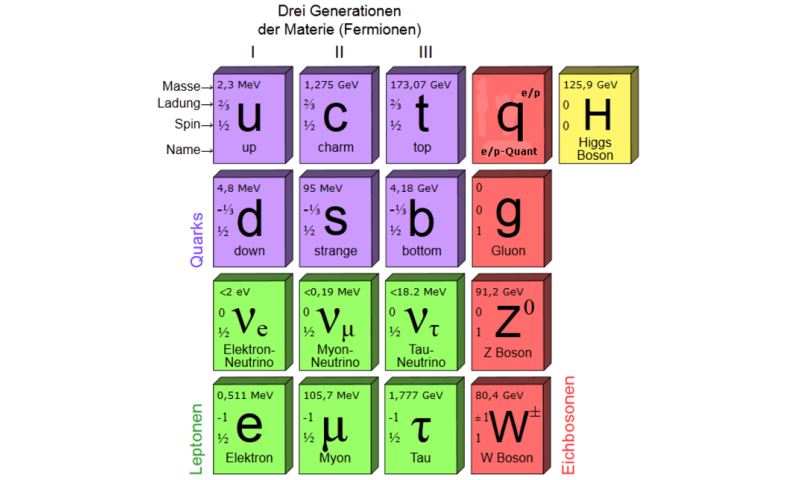
\includegraphics[width=\textwidth,clip]{figures/Chapter1/ParticleTable.png}
    \end{center}
    \caption[标准模型中的基本粒子]{标准模型中的基本粒子}
    \label{fig:ParticleTable}
\end{figure}
其中轻子和夸克为自旋为1/2的费米子,每一种轻子和夸克都有其对应的反粒子。轻子共分为三代(Generation),电子,muon,tau轻子和其对应的中微子分别组成不同的代。每一代轻子和其反粒子都带有被称为轻子数的量子数,轻子严格地遵守轻子数守恒定律。夸克和轻子之间存在着某种对称性,自然,夸克也存在和轻子类似的代的概念,被分为三代夸克,如图 \ref{fig:ParticleTable}所示。除了自旋为1/2的费米子以外,标准模型中还存在着四种规范矢量玻色子作为费米子之间的相互作用的传播子存在。其中光子,$W^{\pm}$以及 $Z^0$玻色子为自旋为1的粒子,而Higgs玻色子为目前唯一自旋为0的玻色子。他的引入源于解决弱相互作用的对称性破缺问题时引入的Higgs场,当粒子与Higgs场相互作用的时候其不再以光速进行传播并且获得质量。而那些不与Higgs场有相互作用的粒子,例如光子、胶子等则保持质量为零。

在量子力学建立之初,人们只是用它来处理粒子这种物质的存在,而对于物理学中另一个很重要的概念——场却没有进行量子化的处理,仍然是经典的,并没有将其和粒子放在同等地位。这就导致有一些问题仍然无法得到很好的解决,例如光电效应、原子发射和吸收光子以及粒子的产生和湮灭等问题。这就让人们开始考虑将量子化的概念从单粒子拓展到场的范围。人们开始尝试把克莱因-高登和狄拉克方程解释成为场方程,即将其中的波函数解释为经典场,从而开始了场的量子化过程。在历史上人们首先对电磁场进行了量子化。得到了处理电磁场相互作用的理论,被称为量子电动力学(Quantum Electrodynamics, QED)。电磁相互作用的传播子为光子。

之后在处理中子的$\beta$衰变的时候,费米意识到电磁相互作用不可能产生这个过程,应该是由于某种新的相互作用而引起了中子的$\beta$衰变过程。这种新的相互作用就是弱相互作用。弱相互作用的强度远弱与电磁相互作用,比电磁相互作用弱了大约$10^{11}$倍。其传播子为$W^{\pm}$以及 $Z^0$。

1937年,汤川秀树类比于描写电磁相互作用的QED理论,提出核力是通过中子和质子之间的一种具有质量的基本粒子来传递的。基于此,汤川预言有一种新的粒子存在,其质量应该介于电子和质子之间,汤川将这种新粒子称为介子(Meson)。后来,汤川预言的这种粒子于1947年被发现,被称为$\pi$介子。至此,粒子世界的主要角色似乎已经齐全了。但在同一年,随着奇异粒子的发现,这种“齐全”的错觉被无情的打破,人们意识到现有的理论不足以解释越来越多的被发现的新粒子。这样人们就有了一个很自然的疑问:这些粒子是否还有着自己的内部结构?

之后夸克模型便被提出用以解释强子的结构问题。1964年由默里·盖尔曼和乔治·茨威格分别独立提出了夸克模型。其认为强子由三种基本的构造单元组成,这三种不同的构造单元被称为具有三种不同味(Flavor)的夸克(Quark),分别是u(up),d(down)和s(strange)夸克。夸克模型很好的解释了强子的生成和湮灭问题,但是在处理一些粒子的组分的时候遇到了困难。按照夸克模型,$\Omega^-$应该有三个s夸克组成且都处于轨道运动的基态,又因为$\Omega^-$的总自旋角动量为$\frac{3}{2}\hbar$,这就要求每一个s夸克的自旋都应该是$\frac{1}{2}\hbar$,明显的违背了泡利不相容原理。基于这个事实,人们开始猜测是否还有一种新的未知的量子数。1965年南部阳一郎研究了这个问题并提出夸克应该有一种新的量子数,他称之为色(Color),从此量子色动力学(Quantum Chremodynamics, QCD)走上了粒子物理学的舞台。


% \subsection{量子色动力学}
量子色动力学被用来描述强相互作用,其传播子为胶子(gluons)。拉式量(Lagrangian)可以表示为:
\begin{equation}
    \mathcal{L}_{QCD} = \bar{\phi}(i \gamma_{\mu} D^{\mu}-m)\phi-\frac{1}{2}G^{a}_{\mu\nu}G^{\mu\nu}_{a}
\end{equation}
其中
\begin{equation}
    G^{a}_{\mu\nu} = \delta_{\mu}A_{\nu}^{a}(x) - \delta_{\nu}A_{\mu}^{a}(x) + gf_{abc}A_{\mu}^{b}(x)A_{\nu}^{c}(x)
\end{equation}
$D^{\mu}$为夸克场与胶子场耦合的协变微分,形式为:
\begin{equation}
    D^{\mu} = \delta_{\mu} - ig\frac{\lambda_{a}}{2}A_{\mu}^{a}(x)
\end{equation}
其中g为QCD耦合常数,$f_{abc}$为$SU(3)_{color}$结构常数,$\phi$为夸克场(对夸克味求和),$\gamma_{\mu}$为狄拉克矩阵,$\lambda_{a}$为盖尔曼矩阵,$G^{a}_{\mu\nu}$为规范不变的场强张量,$A_{\mu}^{a}$为胶子场。量子色动力学有着一些独特的特性,将会在下文中进行介绍。

在自然界中,我们并不能观测到单个存在的夸克,我们只能观测到由多个夸克组成的色中性的强子态(准确的说是色单态)。这意味着夸克和胶子之间的相互作用在距离变远的时候会增长的极快,从而使单个的夸克或者胶子难以存在。在量子色动力学中,势能可以描述为
\begin{equation}
    V_s = -\frac{4}{3}\frac{\alpha_{s}}{r} + kr
    \label{eq:QCDpotential}
\end{equation}
其中$\alpha_{s}$为强相互作用的耦合常数。

第一项在距离较短的时候占主导作用,类似于QED当中的库伦势。随着距离的增加,第二项开始占据主导作用,夸克和胶子之间的作用力成近似线性增加。在深度非弹散射(Deep Inelastic Scattering, DIS)实验中人们发现强子中的夸克和胶子表现出来准自由点状粒子的性质,而根据式\ref{eq:QCDpotential},当r趋近于零的时候$V_s$应该趋近于无穷,这就是知名的朗道极点问题。这个问题在量子色动力学中被由大卫·格罗斯、弗兰克·维尔切克和大卫·波利策提出的渐进自由理论解决。

重整化后的强相互作用力有效耦合常数可以写作:
\begin{equation}
    \alpha_{s}(|q^2|) \equiv \frac{g_s^2(|q^2|)}{4\pi} \approx \frac{12\pi}{\beta_0 ln(|q^2|/\Lambda_{QCD}^2)}
\end{equation}
其中 $\beta_0 = (11n_c-2n_f)$为一个由夸克的颜色数目 $n_c$ 和 夸克的味道数目$n_f$给出来的常数。因为$\beta_0 > 0$,所以$\alpha_{s}$随着$|q^2|$的增加而减小,这显示出来了渐进自由的特性。在实验上可以在不同的能量尺度($Q^2$)的情况下测量强相互作用的耦合常数,其行为和预测的相同,实验上的测量结果如图 \ref{fig:Alpha_S} 所示
\begin{figure}[htb]
    \begin{center}
    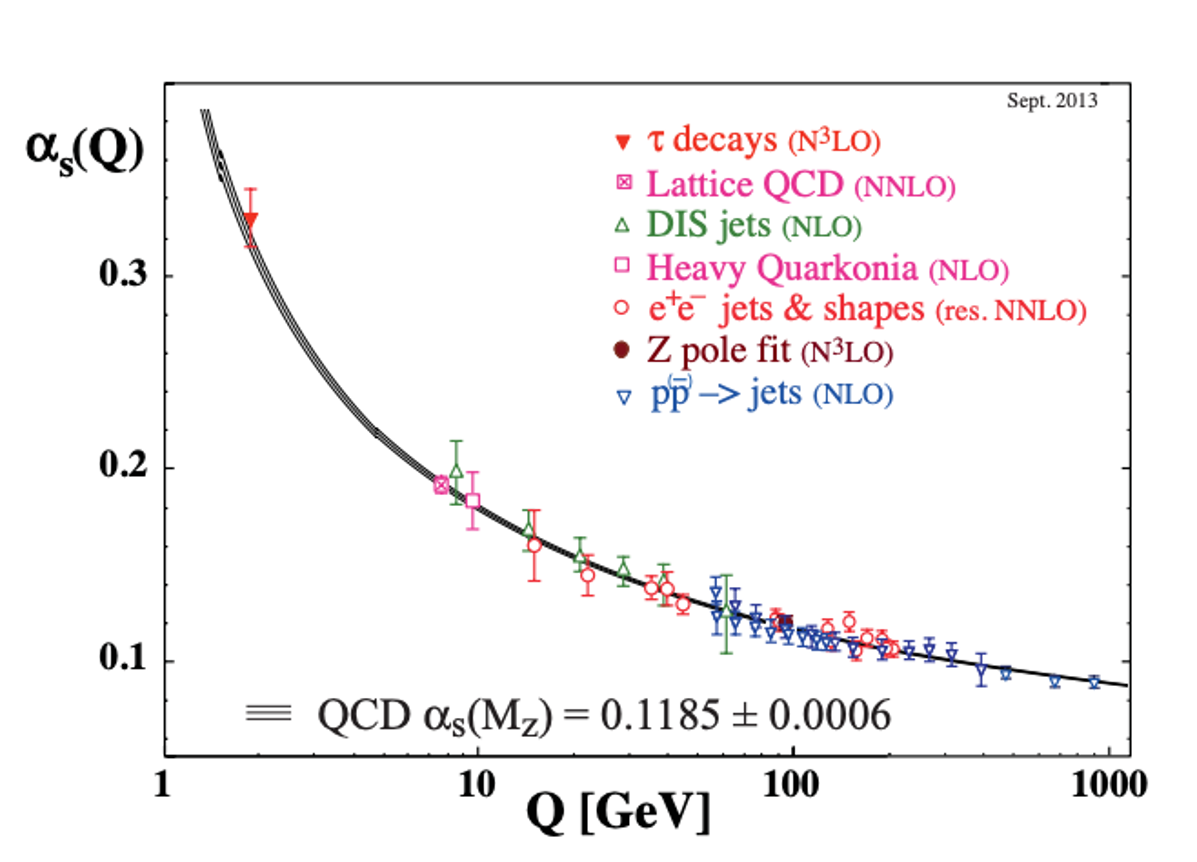
\includegraphics[width=0.7\textwidth,clip]{figures/Chapter1/Alpha_s.png}
    \end{center}
    \caption[$\alpha_s$随能量尺度$Q^2$变化的关系]{$\alpha_s$随能量尺度$Q^2$变化的关系,2014 review of paritcles}
    \label{fig:Alpha_S}
\end{figure}

渐进自由带来了几个有趣的结果。首先在大$Q^2$区间,$\alpha_s \ll 1$。这使得微扰理论在此能量尺度下仍然可以起作用。但随着$Q^2$的减小,$\alpha_s \geq 1$,从而使得微扰量子色动力学不再适用。因此其他的理论被发展出来在此区间进行量子色动力学的计算。目前比较成功的非微扰量子色动力学的计算方式为格点量子色动力学(Lattice QCD)。
% \subsection{渐进自由}
在自然界中,我们并不能观测到单个存在的夸克,我们只能观测到由多个夸克组成的色中性的强子态(准确的说是色单态)。这意味着夸克和胶子之间的相互作用在距离变远的时候会增长的极快,从而使单个的夸克或者胶子难以存在。在量子色动力学中,势能可以描述为
\begin{equation}
    V_s = -\frac{4}{3}\frac{\alpha_{s}}{r} + kr
    \label{eq:QCDpotential}
\end{equation}
其中$\alpha_{s}$为强相互作用的耦合常数。第一项在距离较短的时候占主导作用,类似于QED当中的库伦势。随着距离的增加,第二项开始占据主导作用,夸克和胶子之间的作用力成近似线性增加。在深度非弹散射实验中人们发现强子中的夸克和胶子表现出来准自由点状粒子的性质,而根据式\ref{eq:QCDpotential},当r趋近于零的时候$V_s$应该趋近于无穷,这就是知名的朗道极点问题。这个问题在QCD中被由大卫•格罗斯,弗兰克•维尔切克和大卫•波利策提出的渐进自由理论解决。

重整化后的强相互作用力有效耦合常数可以写作:
\begin{equation}
    \alpha_{s}(|q^2|) \equiv \frac{g_s^2(|q^2|)}{4\pi} \approx \frac{12\pi}{\beta_0 ln(|q^2|/\Lambda_{QCD}^2)}
\end{equation}
其中 $\beta_0 = (11n_c-2n_f)$为一个由夸克的颜色数目 $n_c$ 和 夸克的味道数目$n_f$给出来的常数。因为$\beta_0 > 0$,所以随着$|q^2|$的增加而减小,这显示出来了渐进自由的特性。在实验上可以在不同的能量尺度($Q^2$)的情况下测量强相互作用的耦合常数,其行为和预测的相同,实验上的测量结果如图 \ref{fig:Alpha_S} 所示
\begin{figure}[htb]
    \begin{center}
    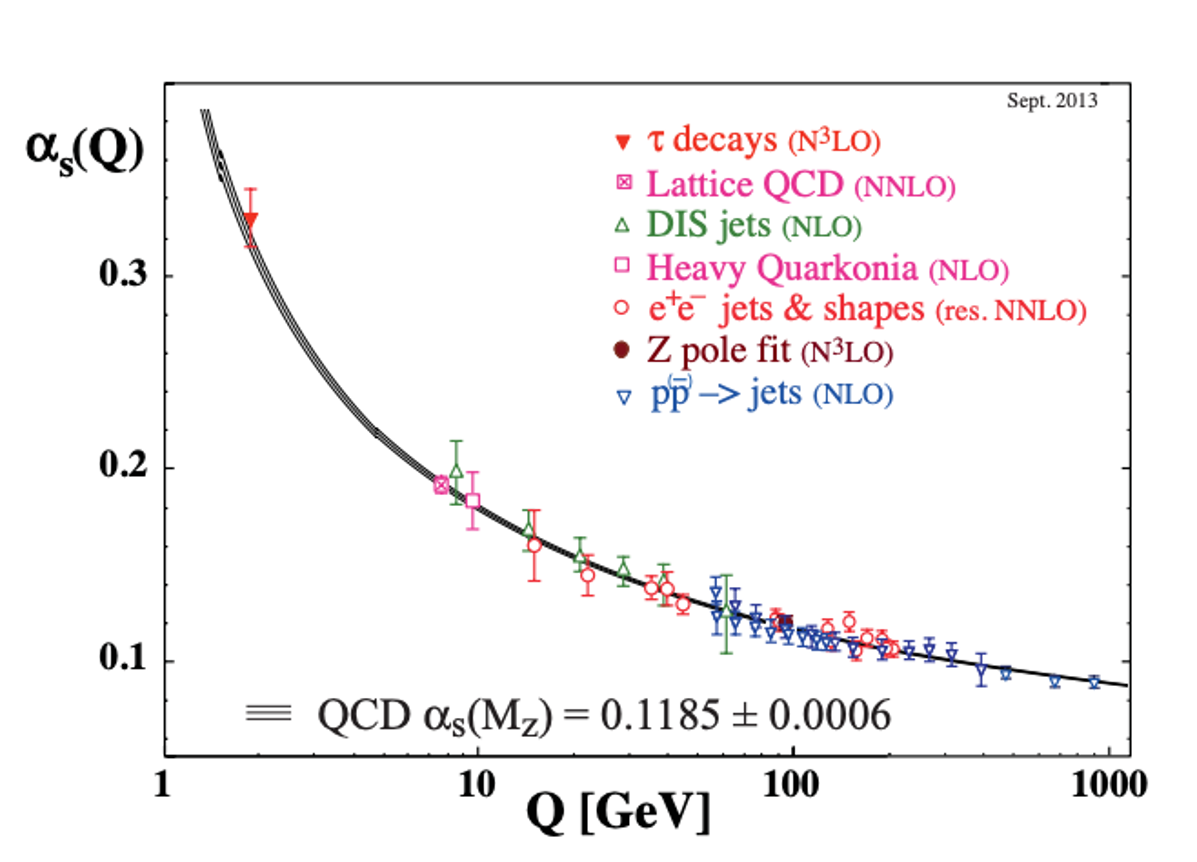
\includegraphics[width=\textwidth,clip]{figures/Chapter1/Alpha_s.png}
    \end{center}
    \caption[$\alpha_s$随能量尺度$Q^2$变化的关系]{$\alpha_s$随能量尺度$Q^2$变化的关系,2014 review of paritcles}
    \label{fig:Alpha_S}
\end{figure}

渐进自由带来了几个有趣的结果。首先在大$Q^2$区间,$\alpha_s \ll 1$。这使得微扰理论在此能量尺度下仍然可以起作用。但随着$Q^2$的减小,$\alpha_s \geq 1$从而使得微扰QCD不再适用。因此其他的理论被发展出来在此区间进行QCD的计算。目前比较成功的非微扰QCD的计算方式为格点QCD(Lattice QCD)。
\section{夸克胶子等离子体}
\label{夸克胶子等离子体}
因为量子色动力学渐进自由的性质,在极端高温下或者密度极高的情况下夸克和胶子可能解禁闭形成新的物质态。类似于等离子体中的电子和原子之间的束缚在高温或者高密的情况下被解除紧闭,电子可以在等离子体中自由移动从而带来很高的电导率一样。在这种新的物质态当中束缚夸克和胶子的强相互作用力被屏蔽,从而使得夸克从强子束缚态中解紧闭形成一种类似于等离子体的状态。这种新的物质的态被称作夸克胶子等离子体(Quark Gluon Plasma, QGP)。根据格点量子色动力学预言,在高温和(或)高密的情况下物质可能发生从强子气到夸克胶子等离子体的相变。和其他物质的相变类似,这种从强子气到夸克胶子等粒子体的相变也有属于自己的相图,如图 \ref{fig:PhaseDiagram} 所示

\begin{figure}[htb]
    \begin{center}
    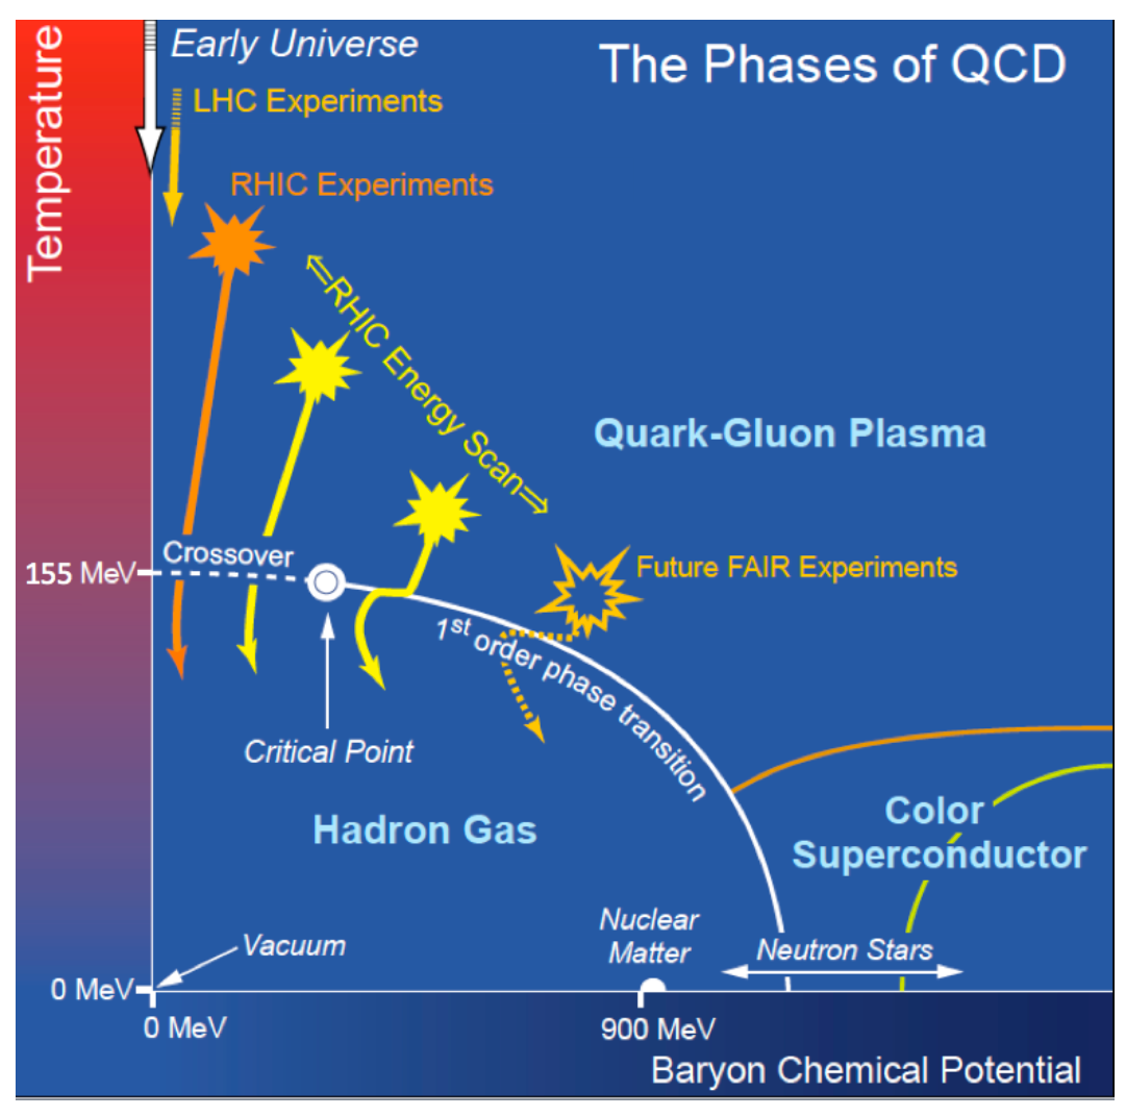
\includegraphics[width=0.7\textwidth,clip]{figures/Chapter1/PhaseDiagram.png}
    \end{center}
    \caption[QGP相图]{QGP相图}
    \label{fig:PhaseDiagram}
\end{figure}

量子色动力学相图给出来的是在温度T和重子化学势$\mu_b$平面上的热力学状态图,从图中可以看出,研究量子色动力学物质相变时,有两种常见的路线。一种是在保持低温的情况下增加夸克物质的密度,沿着这条路线最后达到的物质状态即为中子星内部的物质状态。另一条路线是加热核物质,也可以达到从强子气到夸克胶子等粒子体的相变,这种方式一般通过相对论重离子对撞来实现。
\section{手征对称性}

量子色动力学的拉氏量除了拥有$SU(3)_{color}$和$SU(3)_{flavor}$近似对称性以外还存在着另外一种对称性——手征对称性

当动量转移$Q \sim 1 {\rm~GeV/c}$的时候三种最轻的夸克,上、下和奇异夸克可以被近似地认为质量为零。在这种情况下拉氏量可以被写为:
\begin{equation}
    \label{QCDLagrangian}
    \mathcal{L} = i\bar{\phi}_f \gamma^{\mu} \delta_{\mu} \phi_{f}
\end{equation}

其中f表示夸克的味道。此拉氏量的一个重要的性质是在矢量和轴矢量变换下都有对称性:

\begin{equation}
    \label{Vector}
    \phi \rightarrow e^{i \alpha^{a}_{V}\frac{\lambda_a}{2}} \phi
\end{equation}
\begin{equation}
    \label{AxialVector}
    \phi \rightarrow e^{i \gamma_5 \alpha^{a}_{A}\frac{\lambda_a}{2}} \phi
\end{equation}

矢量和轴矢量的波函数可以用他们的左手或者右手手征分量来表示:

\begin{equation}
    \phi_{R,L} = \frac{1}{2}(1 \pm \gamma_5) \phi
\end{equation}

当我们考虑手征分量的时候变换\ref{Vector}和\ref{AxialVector}可以表示为:

\begin{equation}
    \phi_R \rightarrow e^{i \gamma_5 \alpha^{a}_{R}\frac{\lambda_a}{2}} \phi_R~,~\phi_L \rightarrow \phi_L
\end{equation}
\begin{equation}
    \phi_L \rightarrow e^{i \gamma_5 \alpha^{a}_{L}\frac{\lambda_a}{2}} \phi_L~,~\phi_R \rightarrow \phi_R
\end{equation}

在矢量和轴矢量的变化下我们可以看到一个由手征分量构成的对称性,这种在夸克质量为零的条件下的$SU(N_f)_{R} \times SU(N_f)_{L}$对称性被称作手征对称性。

当夸克质量不为零的时候其可以为视为量子色动力学拉氏量\ref{QCDLagrangian}当中的一个微扰项($\delta\mathcal{L} = -m\bar{\phi}\phi$)。这个微扰项带来了在轴矢量变换下的对称性破缺,因此也打破了手征对称性。对称性破缺可以表现为显式的对称性破缺或者是自发对称破缺。在显式对称性破缺中,对称性的破缺表现为拉氏量在运动方程中对称破缺。但在自发对称破缺中,运动方程依旧保持不变,系统的对称性破缺表现在系统的基态并不是稳定的。

“墨西哥”帽的势能形象地展示了这种自发对称性破缺的状态,如图\ref{fig:MexHat}所示。在这个状态下系统十分的不稳定,任何微小的扰动都可能打破这种平衡,在图中表现为一个很小的扰动就可以让小球从“帽尖”出滑落。这种不稳定性来源于对称性的自发破缺,例如手征对称性。当三种夸克被看作质量为零的时候,我们期待有8种简并的无质量的Goldstone玻色子,其量子数为$J^P = 0^-$。但在实际上是有8种介子拥有此量子数,分别为$\pi^{\pm},\pi^0,K^{\pm},K^0,\bar{K}^0$和$\eta$,手征对称性的自发破缺导致了他们的非零质量。例如这些介子里面最轻的介子$\pi^0$的质量为 $m_{\pi^0} \approx 135~{\rm MeV/c^2}$,但最轻的包含s夸克的介子$K^{\pm}$质量为$m_{K^{\pm}} \approx 494~MeV/c^2$

\begin{figure}[htb]
    \begin{center}
    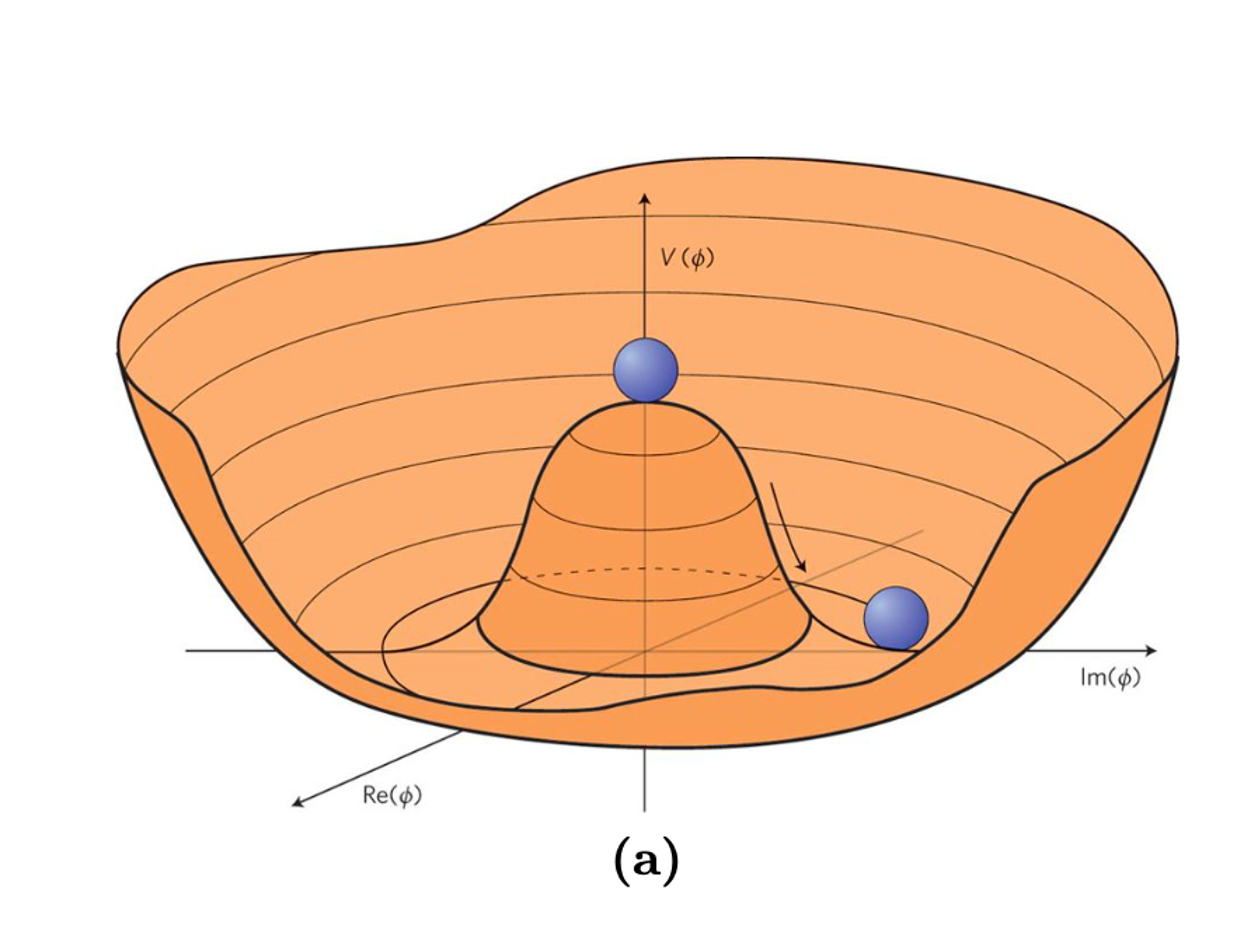
\includegraphics[width=0.7\textwidth,clip]{figures/Chapter1/MexHat.png}
    \end{center}
    \caption["墨西哥帽"势能示意图]{"墨西哥帽"势能示意图}
    \label{fig:MexHat}
\end{figure}

手征对称性的破缺也导致了真空中的夸克凝聚(quark condense)。可以从$\pi$介子的质量和夸克凝聚的关系(Gell-Mann-Oakes-Renner关系)中得到:

\begin{equation}
    m_{\pi}^2 f_{\pi}^2 = -2\bar{m}\langle 0|\bar{q}q|0 \rangle
\end{equation}
其中$\bar{m} \approx 6~ {\rm MeV/c^2} $是u和d夸克的平均质量。从这个关系式中我们可以看到真空中的夸克凝聚的值$\langle 0|\bar{q}q|0 \rangle \approx (-250 {\rm~MeV})^3$。这也是手征对称性破坏的标志之一。

在实验上对手征对称恢复的观测可以通过测量手征多重态的质量分布来做到,例如$\rho^0(770)$和$a_1(1260)$。如果没有手征对称性破缺这两个态将会是简并的,然而在实验的测量中却发现他们两个的质量差别很大:$m_{\rho^0} \approx 770 ~{\rm MeV/c^2}$, $m_{a_1} \approx 1260 ~{\rm MeV/c^2}$。这种质量的差别不能简单的被u夸克和d夸克的质量差别来描述,很可能由手征对称性的破缺带来。

人们预期这种夸克凝聚态会在高温($T > T_c^{chiral}$)、高密($n > n_c^{chiral}$)的条件下发生改变。因此人们期待在这种条件下可以看到从带有自发手征对称性破缺强子物质态到手征恢复的物质态的转变。但需要注意的是手征恢复的的相变条件和量子色动力学物质解禁闭的相变条件并不相同,人们预期手征对称恢复的相变温度要高于夸克胶子等离子体的相变温度,即在相同的重子势下,$T_c^{chiral} > T_c^{QGP}$。这就意味着夸克胶子等离子体可能在手征对称恢复没有达到的情况下存在,同时也意味着存在手征对称恢复的时候夸克和胶子一定是解禁闭的。在实验上手征对称恢复一个很重要的观测量便是$\rho^0$和$a_1$质量的简并,对他们质量谱的测量是我们直接对手征对称恢复进行观测的一个很重要的手段。

\section{相对论重离子对撞}

正如 \ref{夸克胶子等离子体} 一节中所提到的一样,在实验上产生夸克胶子等离子体的主要方式为相对论重离子对撞。通过控制相对论重离子对撞的离子类型和对撞中每核子对的能量($\sqrt{s_{NN}}$),可以在QCD的相图中得到不同的T-$\mu_b$曲线。从而成为探索QCD相图的有力的工具。以相对论重离子对撞机(Relativistic Heavy-Ion Collider, RHIC)为例。常用的对撞系统为金-金对撞,最高可以达到 \sNNerbai 的对撞能量,在这种情况下金离子可以被加速到大约99.99\%的光速。

在相对论情况下球状的原子核会收缩成扁平的盘状,当他们在束流管中交汇时就可能发生对撞。一个很重要的描述对撞对心程度的参数为碰撞参数b,其定义为两个核中心之间的距离,参见图 \ref{fig:ImpactParameter}。当$b \approx 0$时称为“中心(Central)”对撞,当$b \approx 2R$时称为“偏心(Peripheral)”对撞。但在实验上我们无法直接观测到一次对撞发生时的碰撞参数,所以我们用一个基于带电粒子多重数(在某区间内的带电粒子数,Reference Multiplicity,RefMult)的中心度(Centrality)定义来描述对撞的对心程度。Glauber模型被用来计算对撞发生后带电粒子多重数的分布,在Glauber模型中带电粒子多重数和中心度关系的示意图见图 \ref{fig:Centrality}。除了中心度,还有一些常用的量也被用来描述对撞的对心程度,例如参加对撞核子数($N_{part}$),二元碰撞数($N_{bin}$)以及核几何重叠函数(Geometrical nuclear overlap function, $T_{AA} = N_{coll}/\sigma_{NN}^{inel}$)等。

\begin{figure}[htb]
    \begin{center}
    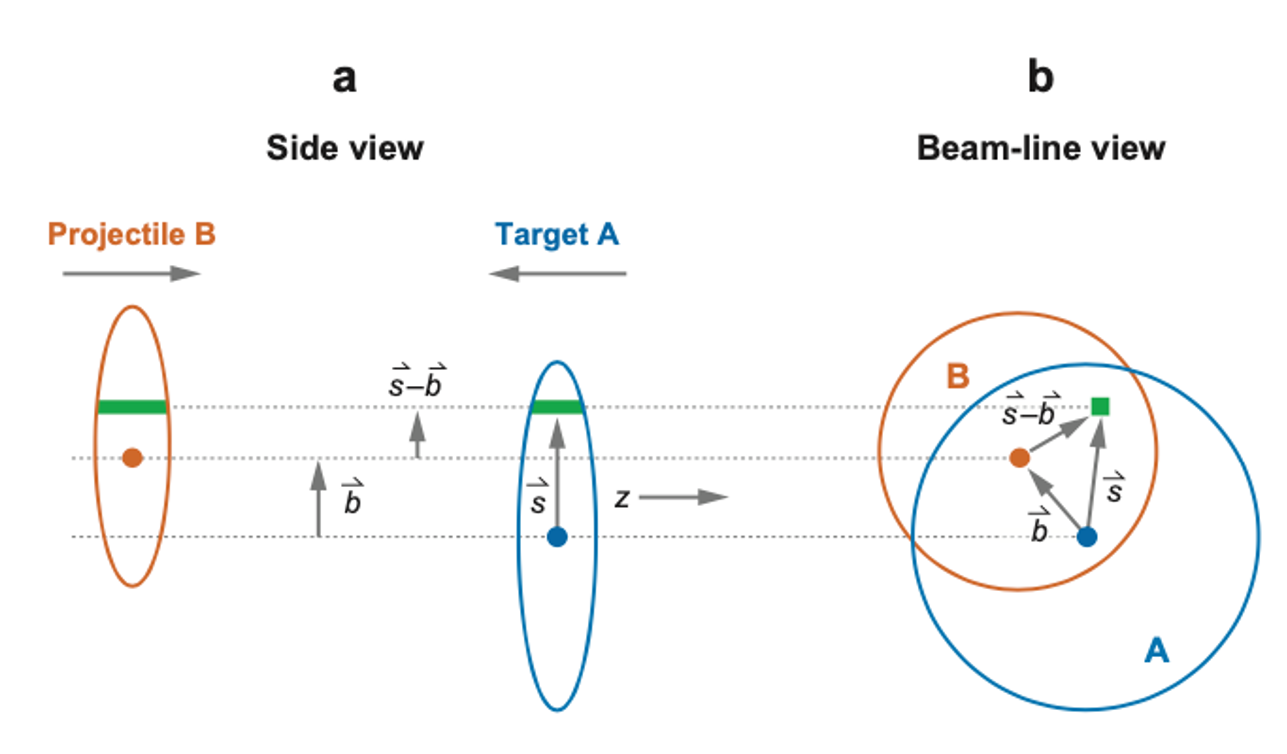
\includegraphics[width=0.7\textwidth,clip]{figures/Chapter1/ImpactParameter.png}
    \end{center}
    \caption[重离子对撞中的碰撞参数示意图]{重离子对撞中的碰撞参数示意图,其中图(a)为侧视图,图(b)为沿着束流方向视图。$\overrightarrow{b}$为碰撞参数,$\overrightarrow{s}$为Glauber模型中表示到核子中心距离的向量}
    \label{fig:ImpactParameter}
\end{figure}

\begin{figure}[htb]
    \begin{center}
    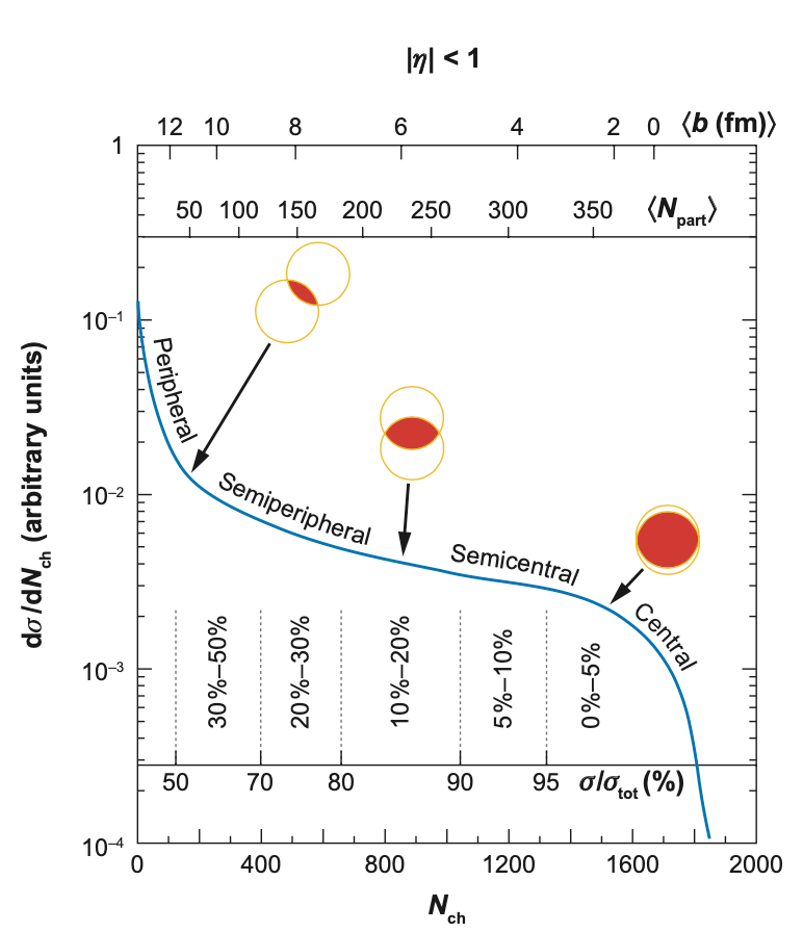
\includegraphics[width=0.6\textwidth,clip]{figures/Chapter1/Centrality.png}
    \end{center}
    \caption[中心度定义示意图]{Glauber模型中末态可观测的带电粒子径迹数和碰撞参数以及$N_{part}$的关系示意图,图中的值为定性的分布,并不是实际的测量值}
    \label{fig:Centrality}
\end{figure}

在一次重离子对撞发生以后所产生的QCD物质如何演化是重离子对撞物理中最为感兴趣的问题。对撞发生后的系统演化的示意图见图 \ref{fig:HIC}。在碰撞的早期发生的过程主要是核子和核子之间(或者说核子内的部分子)之间的散射过程,主要是有着小横动量转移的“软(soft)”过程。虽然数量较少但仍有一部分粒子发生了大横动量转移的过程(“硬(hard)”过程),产生了有着较高横动量($p_T$)的粒子,这些硬过程对我们的研究十分重要。碰撞发生的早期阶段被称作“预平衡”阶段,目前有多种理论模型来描述这个阶段,例如色玻璃凝聚模型(Color Glass Condensate, CGC),但我们对他们的动力学状态仍不是十分清楚。在碰撞发生后的大约 1 fm/c 之后,发生对撞的两个离子相互离开,但是在离子和离子重叠的区域沉积下了大量的能量,在这个时间段能量密度可以达到大约 $12 {\rm GeV/fm^{-3}}$,远大于强子内的能量密度,因此对撞中产生的夸克和胶子等难以保持束缚的强子态,从而组成一种新的物质的态,正是我们之前提到的夸克胶子等离子体。近些年来一些粘性流体力学的模型被用来描述QGP的性质并且取得了巨大的成功。

在之后,QGP向各个方向扩张同时冷却,当系统的温度接近$T_c \approx 150 {\rm MeV}$的时候系统开始冷却,首先夸克和胶子强子化生成各种强子,从夸克胶子等离子体相向强子气相转变,在这个过程中强子和强子之间仍可以发生非弹性散射,来改变粒子的种类。当强子的产额基本固定之后我们称这个状态为化学冻结(Chemical freeze-out)。 之后随着温度的进一步降低和系统的扩张,粒子之间的距离大于粒子散射的平均自由程时,粒子的动力学性质也几乎不再改变,这个状态被称为动力学冻结(Kinetic freeze-out)。动力学冻结发生后粒子的动量谱便不再改变并且自由地向各个方向飞出并被探测器探测到。

可以看到,整个QGP的演化时间极短,远小于现今的探测器可以做到的最小的时间分辨,这意味着我们需要从探测到的末态粒子来反推QGP的性质和初始状态,这就要求我们需要找到一些合适的物理探针来进行QGP的研究。从图 \ref{fig:HIC} 中可以看到,光子和电子可以在QGP演化的整个过程中产生,同时其又几乎不与强子物质发生反应,可以在末态被探测到并且受到较小的介质影响。是一个研究QGP的理想探针,将在下一节中进行详细的介绍。

% \begin{figure}[htb]
%     \begin{center}
%     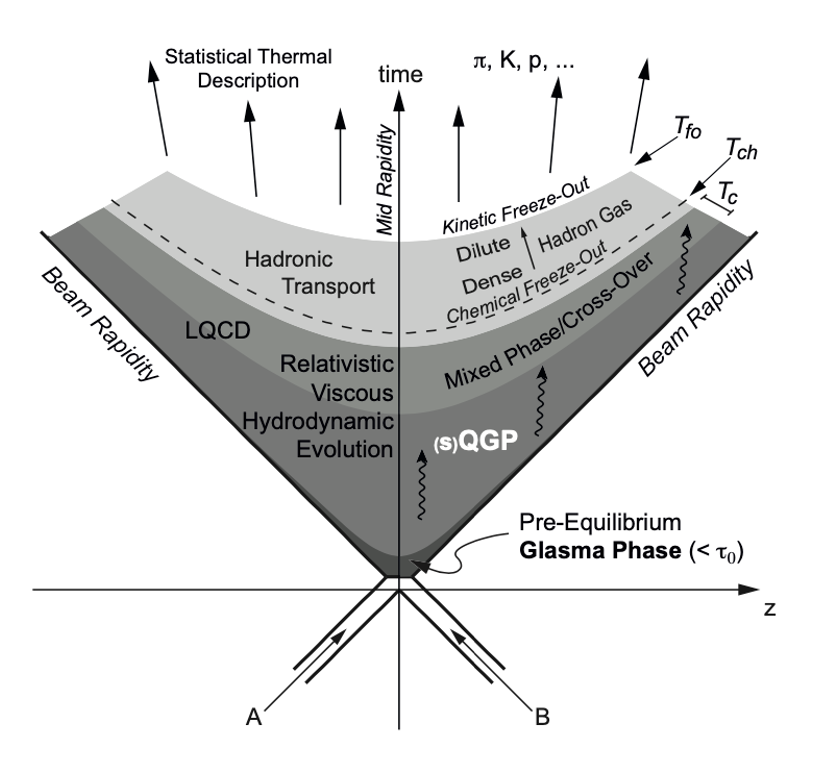
\includegraphics[width=0.8\textwidth,clip]{figures/Chapter1/HIC.png}
%     \end{center}
%     \caption[重离子对撞演化示意图]{一次重离子对撞发生后的系统演化的光锥示意图。主要的相和演化步骤以及对应的温度在图的右侧标出,成功的描述这种演化的模型在图的左侧被标出}
%     \label{fig:HIC}
% \end{figure}

\begin{figure}[htb]
    \begin{center}
    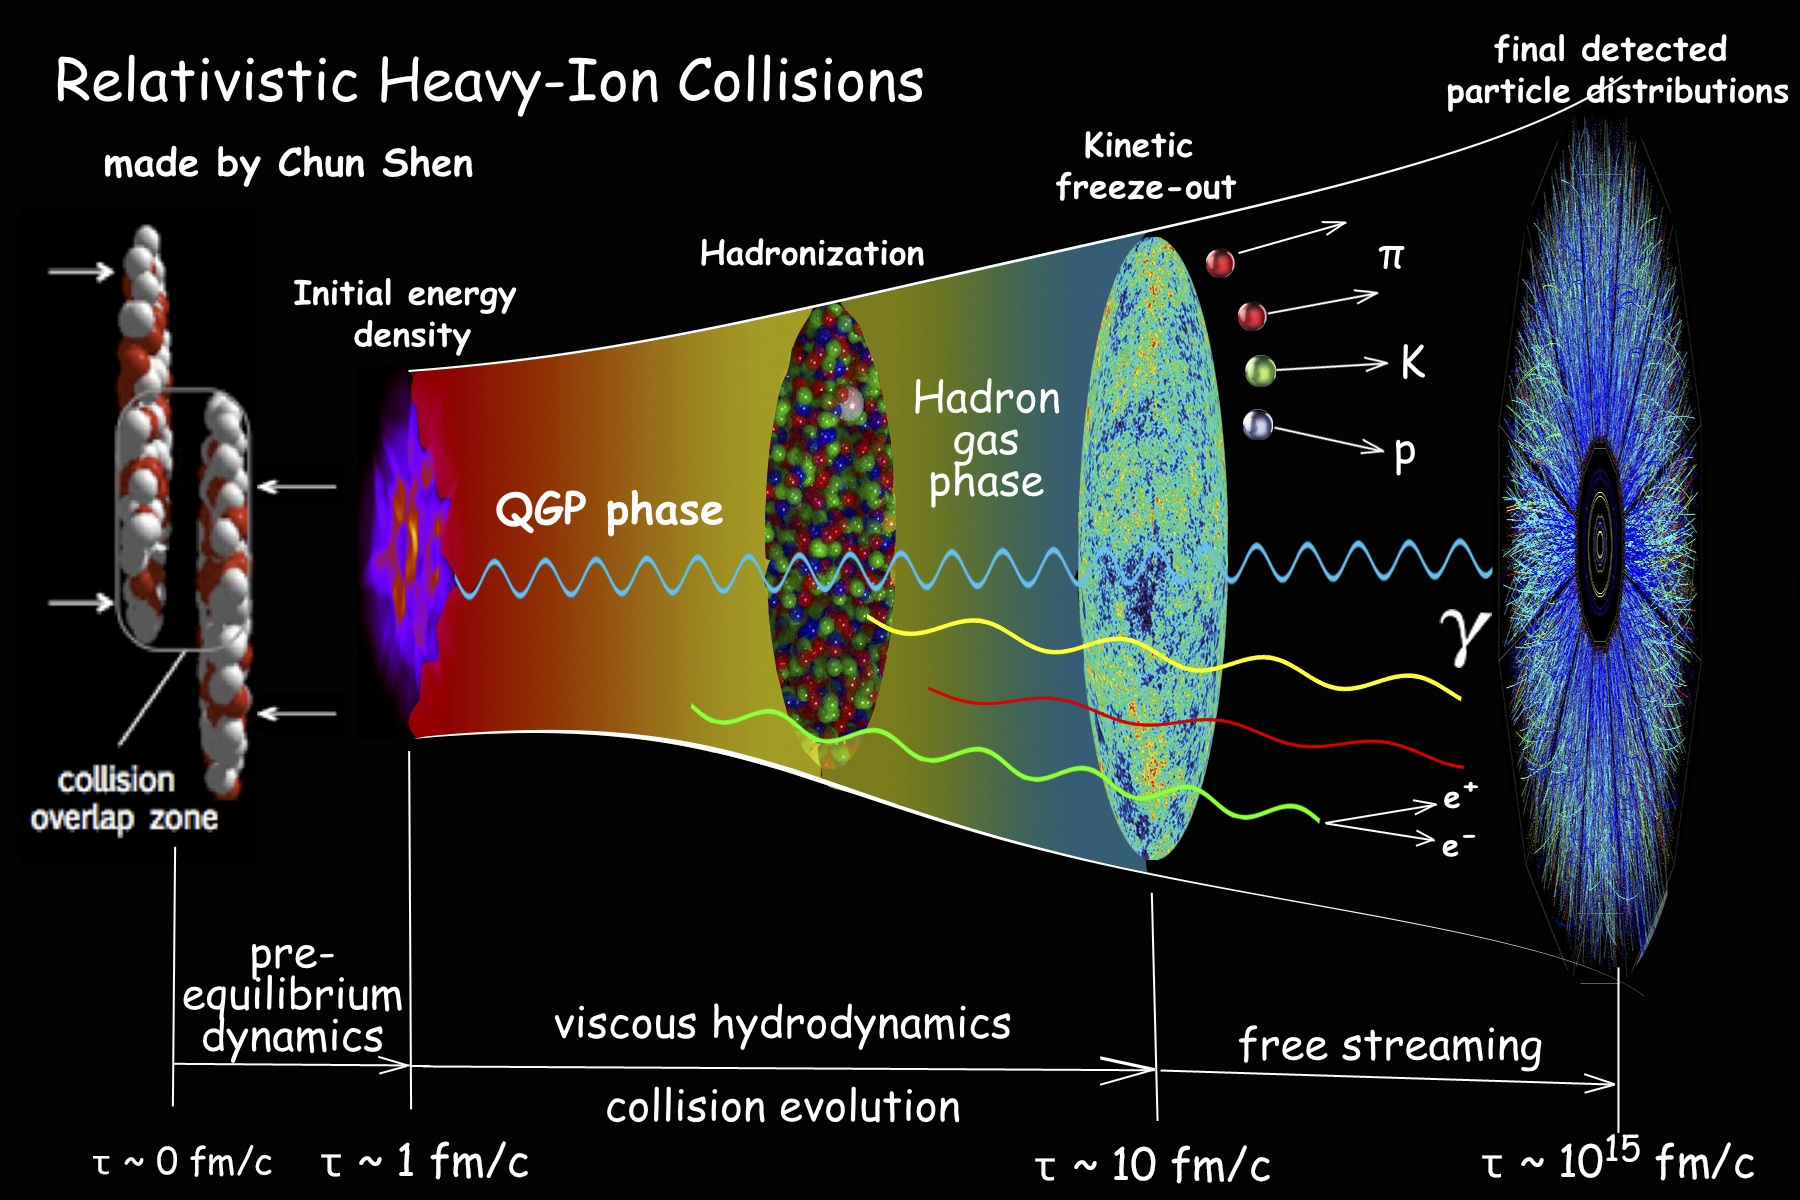
\includegraphics[width=0.8\textwidth,clip]{figures/Chapter1/little_bang-10wt2pd.jpeg}
    \end{center}
    \caption[相对论重离子演化示意图]{一次重离子对撞发生后的系统演化的示意图。图源https://u.osu.edu/vishnu/2014/08/06/sketch-of-relativistic-heavy-ion-collisions/}
    \label{fig:HIC}
\end{figure}
\section{相对论重离子对撞中的双轻子}

\subsection{相对论重离子对撞中的双轻子产生}

如上节中提到的那样,双轻子是如今相对论重离子对撞物理中一个很重要的电磁探针。通过双轻子我们可以有手段对介质初期的演化进行研究。对于双轻子来说,其不变质量谱是一个重要的物理观测量,在 不同的质量区间有着不同的产生机制。同时也是唯一一种可以直接观测QCD介质中介质修正谱方程(In-medium spectral function of QCD medium)的手段。接下来会对不同质量区间的的双轻子产生机制进行简要的介绍。

对于整个的双轻子不变质量谱,根据其产生机制和物理目标不同我们主要将其分为三个不同的质量区间,分别是低质量区间(Low Mass Region, LMR, $M_{ee} < M_{\phi}$ ),中等质量区间(Intermediate Mass Region, IMR, $M_{\phi} < M_{ee} < M_{J/\psi}$)和高质量区间(High Mass Region, HMR, $M_{J/\psi} < M_{ee}$)。双轻子的不变质量越重,其产生于系统演化的越早期。

\begin{figure}[htb]
    \begin{center}
    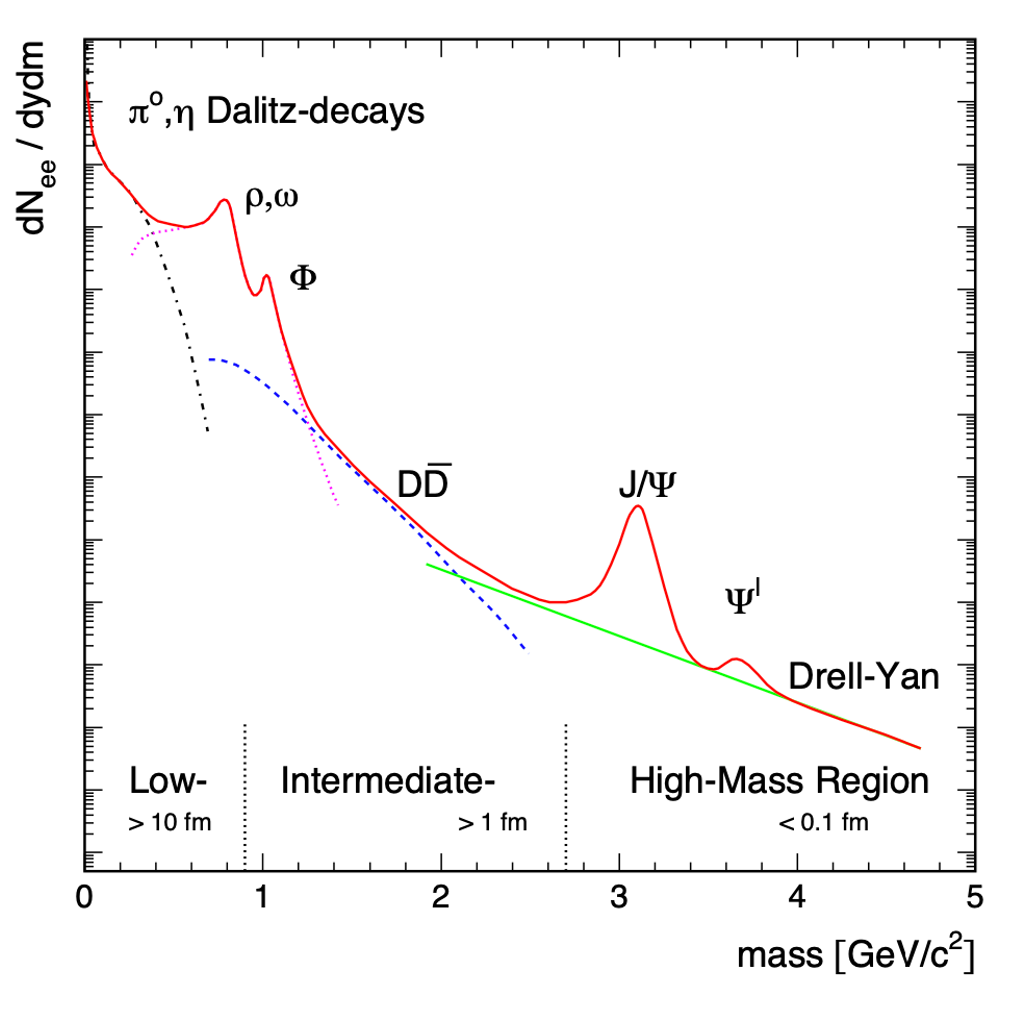
\includegraphics[width=0.8\textwidth,clip]{figures/Chapter1/DileptonSpectra.png}
    \end{center}
    \caption[双轻子不变质量谱示意图]{双轻子不变质量谱的质量区间划分和主要双轻子来源}
    \label{fig:DileptonSpectra}
\end{figure}

在高质量区间,双轻子主要来自于碰撞发生早期的部分子硬散射过程,例如Drell-Yan过程($q\bar{q} \rightarrow \gamma^*/Z \rightarrow l^{+}l^{-}$),重味夸克($b\bar{b}$)的半轻子衰变(semi-leptonic heavy flavor decays)以及重味夸克偶素的衰变($J/\psi, \psi(2S)$和$\Upsilon$)。

夸克偶素因为德拜屏蔽(Debye screening)在高温介质中解离成为夸克的过程被认为是夸克胶子等离子体存在的标志之一,因此夸克偶素在重离子对撞中的产额压低(suppression)是近些年来重离子对撞物理中一个十分令人感兴趣的课题。在离子-离子对撞中夸克偶素截面的核修正因子(Nuclear modification factor, $R_{AA}$)的测量中观测到了这种产额压低的存在。同时在RHIC上也观测到到了在前向快度区间($1.2 < |y| < 2.2$)相比于中间快度区间($|\eta <0.35|$)有着更强的产额压低,这意味着除了色屏蔽以外可能有着其他的机制对夸克偶素的产额有着影响。目前常见的理论有夸克偶素的重结合(recombination),冷核物质效应(Cold Nuclear Matter effect, (CNM))等。

在中等质量区间,双轻子的主要来源是c(charm)夸克的半轻子衰变以及夸克胶子等离子体的热辐射。在初始硬过程中产生的背对背的$c$和$\bar{c}$各自独立地强子化为$D$和$\bar{D}$介子,这些介子再进行半轻子衰变生成轻子。在强子化的过程中,这些强子继承了初始的$c\bar{c}$夸克对的关联性并将其带到了最后两个半轻子衰变的组成的轻子对当中。但因为介质对c夸克的影响,轻子和轻子之间的关联性将会发生一定的改变,对最后的不变质量谱产生影响。需要注意的是,在中等质量区间这部分来源于粲夸克半轻子衰变的双轻子产额远高于来源于夸克胶子等离子体热辐射的双轻子产额,这使得想要在此质量区间抽取来源于夸克胶子等离子体的热辐射的双轻子产额变得十分困难。给实验上测量带来了巨大的挑战。

对于小质量区间来说,双轻子对的主要来源是各种介子的衰变。在诸多介子的质量谱当中,$\rho^0$的质量谱在介质当中的演化是我们最感兴趣的部分。因为$\rho^0$的寿命为大约1.3 fm/c,远小于夸克胶子等离子体的寿命(在RHIC最高能量下的“中心”碰撞中大约为 10 fm/c),其不变质量谱明显地受到与介质相互作用的影响而发生了改变。这个相互作用主要来源于 $\pi^+ + \pi^- \leftrightarrow \rho$ 道的强耦合。这个不变质量谱的改变和手征对称性恢复相关。当手征对称性恢复发生的时候,两个不同的手征多重态的质量(如$\rho(770)$和$a_1(1260)$)发生简并。在实验上测量$a_1(1260)$的质量谱是很困难的,所以我们可以通过测量$\rho(770)$来对手征对称性的恢复进行测量。尽管相对于$a_1(1260)$的测量相对来说容易一些,在双轻子测量中测量$\rho(770)$质量谱依旧十分困难。这是因为在低质量区间除了由$\rho(770)$衰变产生的双轻子对,还有大量的来源于其他介子例如$\pi^0, \eta, \eta^\prime, \omega, \phi$等介子的衰变的双轻子对。为了抽取$\rho(770)$的不变质量谱,其他介子的不变质量谱需要通过某种手段从总的不变质量谱中扣除。对于所有已知产额的介子,我们可以通过模拟的方式来得到其在不同能量不同对撞系统下的不变质量谱,这样我们就可以从总的不变质量谱中扣除这些已知产额的介子的谱,剩下的便是我们想要测量的介子的质量谱。因为这种将多种介子的不变质量谱的模拟混合的方式就像调制鸡尾酒的时候将多种基酒混合在一起,这个模拟的方法被称作“强子衰变模拟(hadronic cocktail)”,将会在双轻子分析一章中进行详细的讨论。

综上所述,通过测量双轻子的不变质量谱可以达到丰富的物理目标,在过去的几十年中各个合作组在不同能量下对多种对撞系统进行了双轻子谱的测量,在接下来的一个小节中将对近些年来双轻子测量进行一个简单的回顾。
\subsection{双轻子测量历史}

在历史上,许多实验都进行过双轻子的测量,并且得到了十分显著的成果,在这一小节中将会对历史上的双轻子测量进行一个简要的回顾。

\subsubsection{NA45实验}
环形切伦科夫电子能谱仪(Cherenkov Ring Electron Spectrometer, CERES, aka NA45),即NA45实验是位于欧洲核子中心(Conseil Européenn pour la Recherche Nucléaire, CERN)的超级质子同步加速器(Super Proton Synchrotron, SPS)上的能谱仪。其可以用两个对称的环状切伦科夫探测器来对电子进行鉴别从而测量双电子谱。NA45首先对p+Be和p+Au系统低质量区间的双电子谱进行了测量,结果如图 \ref{fig:NA45pA} 所示。可以看到进行了背景扣除的双电子谱可以被强子衰变模拟很好地描述。同时这两个测量表明强子衰变模拟可以很好的描述初始的冷核物质效应。

\begin{figure}[htb]
    \centering
    \begin{subfigure}[b]{0.47\textwidth}
        \centering
        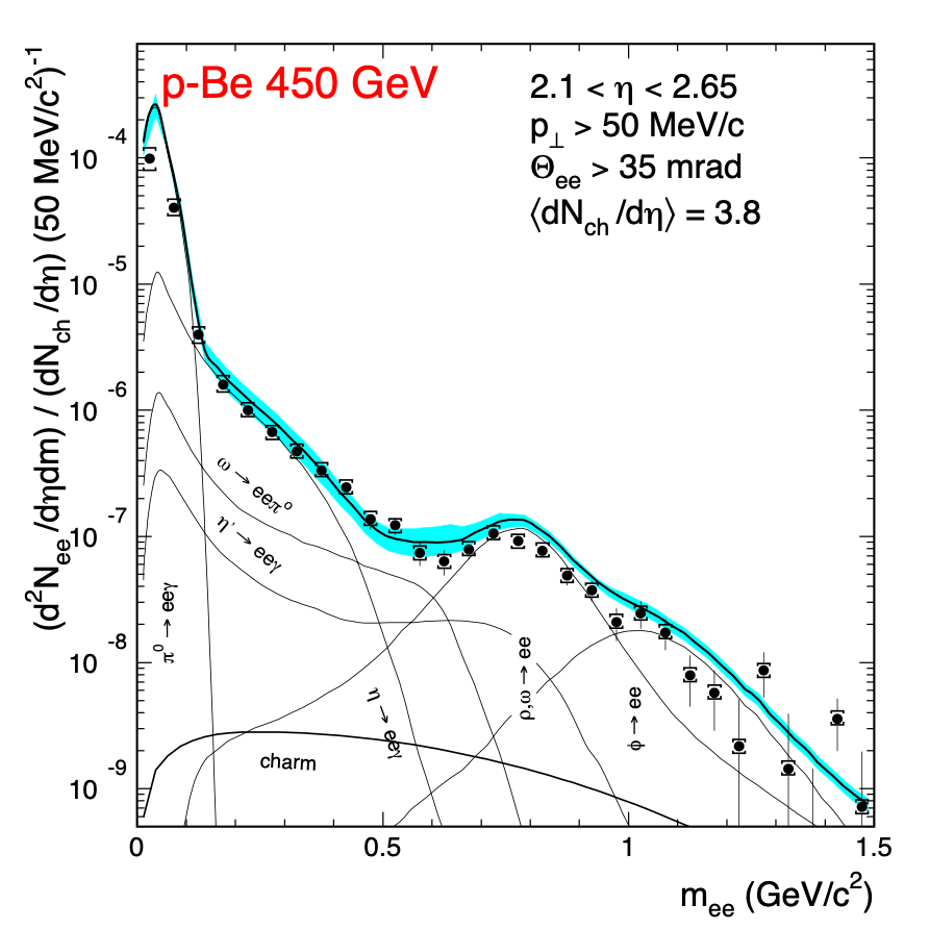
\includegraphics[width=\textwidth,clip]{figures/Chapter1/NA45pBe.png}
        \caption{}
        \label{fig:NA45pBe}
    \end{subfigure}
    \hfill
    \begin{subfigure}[b]{0.47\textwidth}
        \centering
        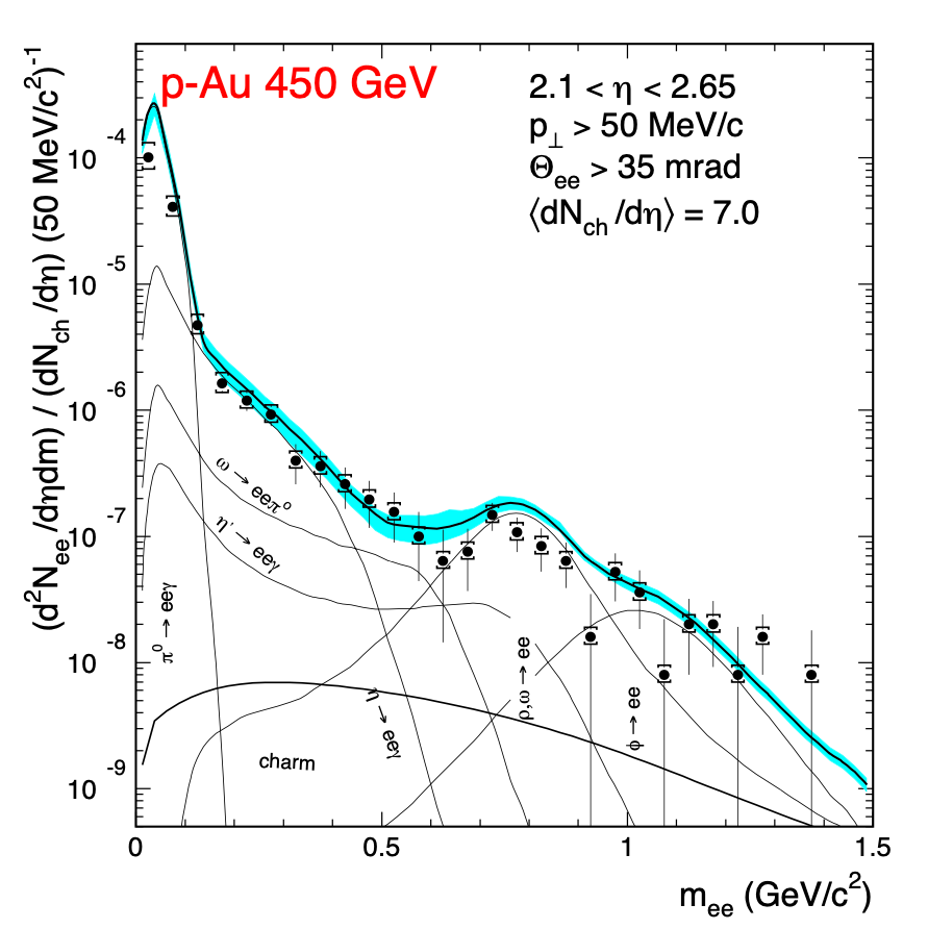
\includegraphics[width=\textwidth,clip]{figures/Chapter1/NA45pAu.png}
        \caption{}
        \label{fig:NA45pAu}
    \end{subfigure}
    \caption[NA45实验p+Be及p+Au对撞中低质量区间双电子谱]{NA45实验450 GeV p+Be \ref{fig:NA45pBe} 以及p+Au \ref{fig:NA45pAu} 对撞中的双电子谱。图中黑色实心圆点为数据点,黑线为强子衰变模拟结果。青色的error band代表了强子衰变模拟的系统误差。}
       \label{fig:NA45pA}
\end{figure}

之后NA45实验也对重离子对撞中的双电子谱进行了测量,图 \ref{fig:NA45SAu} 和图 \ref{fig:NA45PbAu} 分别展示了在200 AGeV 的硫-金对撞和 158 AGeV 铅-金对撞中的双电子谱。在这两个测量中可以看到数据点喝强子衰变模拟相比都有明显的额外产额增强。理论家们提出了一些模型来试图通过热辐射来解释这些额外产额,例如$\pi^+ + \pi^- \leftrightarrow \rho \rightarrow e^+ + e^-$过程。但当这些模型使用真空中的$\rho$质量谱的时候人们发现并不能很好的描述数据。这使得两种关于介质中的$\rho$不变质量谱的模型被提出来用以描述数据,分别是dorpping $\rho$ mass model 和 broadened $\rho$ model。这两种模型和数据的比较见图 \ref{fig:NA45PbAu}。但受限于统计,NA45的结果无法对这两种模型是否能很好的描述数据进行有效的分辨。这两种模型的比较直到后来NA60的更高精度双 \muon 谱测量结果出炉后才有了一个相对明确的结论。

\begin{figure}[htb]
    \centering
    \begin{subfigure}[b]{0.47\textwidth}
        \centering
        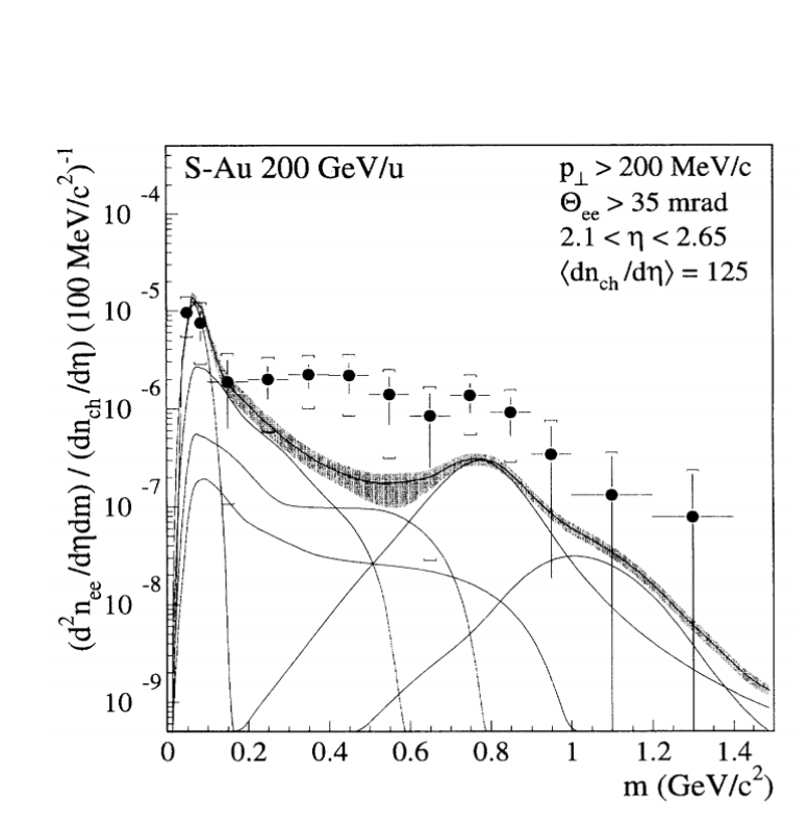
\includegraphics[width=\textwidth,clip]{figures/Chapter1/NA45SAu.png}
        \caption{}
        \label{fig:NA45SAu}
    \end{subfigure}
    \hfill
    \begin{subfigure}[b]{0.47\textwidth}
        \centering
        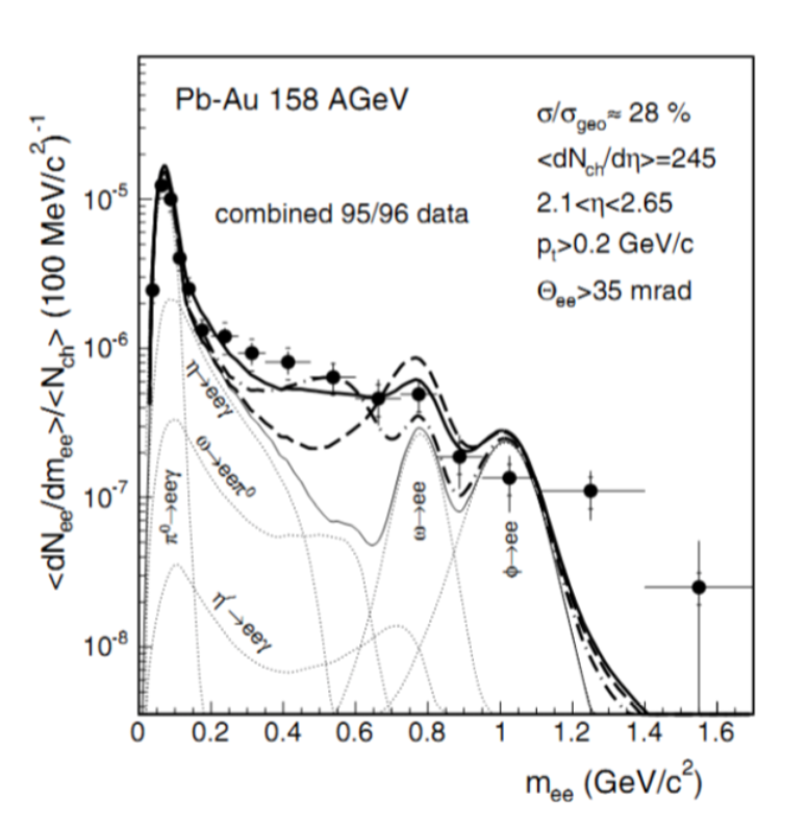
\includegraphics[width=\textwidth,clip]{figures/Chapter1/NA45PbAu.png}
        \caption{}
        \label{fig:NA45PbAu}
    \end{subfigure}
    \caption[NA45实验200 AGeV 硫-金及 158 AGeV 铅-金对撞中的双电子谱]{NA45实验中测得的200 AGev 硫-金对撞中的双电子谱\ref{fig:NA45SAu}和158 AGeV 铅-金对撞中的双电子谱\ref{fig:NA45PbAu}。右图中虚线为强子衰变模拟+真空中$\rho$双电子谱的模拟结果。两种不同的描述$\rho$的不变质量谱变化的模型一并被放入了图中,分别为在图中以点划线表示的dorpping $\rho$ mass model和以粗实线表示的broadened $\rho$ model。}
       \label{fig:NA45AA}
\end{figure}

\subsubsection{NA60实验}

NA60实验为超级质子同步加速器上的固定靶实验。因为NA60实验所拥有的高精度的 \muon 谱仪和顶点探测器,使得其有能力进行高质量分辨(~20 $\rm{MeV/c^20}$)和高位置分辨($ \sigma_x < 10 \mu m$,$\sigma_x < 15 \mu m$)的测量。基于高精度的实验设置,NA60可以有效的去除来自于弱衰变(例如 $\pi^{\pm} \rightarrow \mu^{\pm} + \nu_{\mu}(\bar{\nu}_{\mu})$和$K^{\pm} \rightarrow \mu^{\pm} + \nu_{\mu}(\bar{\nu}_{\mu})$)的背景和来源于重味半轻子衰变的 \muon 。NA60对 \sNN = 17.3 GeV 铟-铟对撞中的双 \muon 谱进行了测量,在全部中心度区间和“半中心”(semicentral)中心度区间的测量结果分别如图 \ref{fig:NA60NoCen} 和 \ref{fig:NA60SemiCentral}所示。
在“半中心”对撞的测量结果在扣除强子衰变模拟(不含 $\rho$)后和不同理论模型预测的$\rho$的不变质量谱进行了比较,因为该测量有着很高的精度,结果可以对理论模型的结果进行很好的约束。可以看到dropping $\rho$ 模型并不能描述数据而 broaden $\rho$ 模型可以在 $0.2 <  M_{\mu\mu} < 0.8~{\rm GeV/c^2} $的质量区间里很好的描述数据。
\begin{figure}[htb]
    \centering
    \begin{subfigure}[b]{0.47\textwidth}
        \centering
        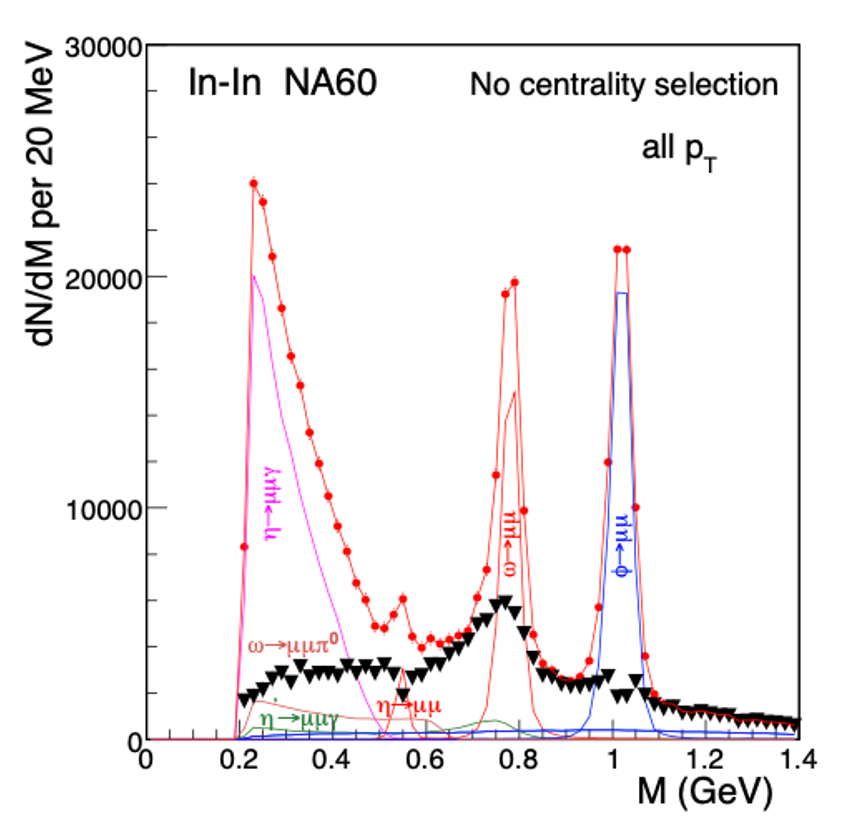
\includegraphics[width=\textwidth,clip]{figures/Chapter1/NA60NoCen.png}
        \caption{}
        \label{fig:NA60NoCen}
    \end{subfigure}
    \hfill
    \begin{subfigure}[b]{0.47\textwidth}
        \centering
        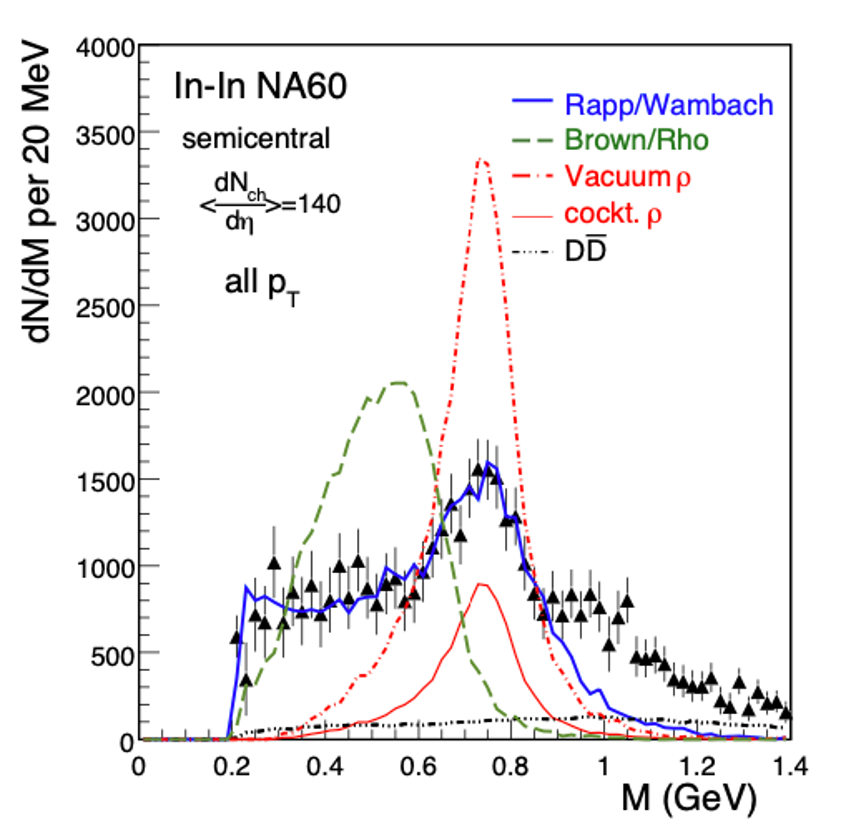
\includegraphics[width=\textwidth,clip]{figures/Chapter1/NA60SemiCentral.png}
        \caption{}
        \label{fig:NA60SemiCentral}
    \end{subfigure}
    \caption[NA60实验\sNN = 17.3 GeV 铟-铟对撞中的双 \muon 谱]{NA60实验\sNN = 17.3 GeV 铟-铟对撞中的双 \muon 谱。左图中未进行中心度筛选的双 \muon 谱,其中红色圆点为未扣除强子衰变模拟的双 \muon 谱,黑色三角为扣除强子衰变模拟后的双 \muon 谱。右图为扣除强子衰变模拟后在“半中心”中心度下的双 \muon 谱。来自不同模型预测的 $\rho$ 的产额在途中以不同形式的线标出。}
       \label{fig:NA60DiMuon}
\end{figure}

在更高的质量区间($M_{\mu\mu} > 0.8~{\rm GeV/c^2}$),双 \muon 的额外产额并不能被任何一种有关 $\rho$ 不变质量谱在介质中的修正模型来描述。在高精度的顶点测量探测器的帮助下NA60实验可以对双轻子的额外产额来源进行分析。经过分析,重味夸克的半轻子衰变和Drell-Yan过程被认为不是额外产额的主要来源。因为统计量足够,NA60进一步对不同的质量区间进行了$m_{T}~(m_{T} = \sqrt{p_T^2 + m^2})$谱的研究。在不同的质量区间用一个指数分布来拟合$m_T$谱,拟合方程为:$1/m_{T}*dN/dm_{T} \propto exp(-m_{T}/T_{eff})$。其中的反斜率参数$T_{eff}$可以被解释为介质的有效温度。在不同质量区间中的有效温度的拟合如图 \ref{fig:NA60T}所示。$T_{eff}$在大约1 GeV处的突然降低表明用强子产生并不能很好的解释在中等质量区间的双轻子额外产额,更自然的解释是这部分额外产额来源于介质的热辐射。

\begin{figure}[htb]
    \begin{center}
    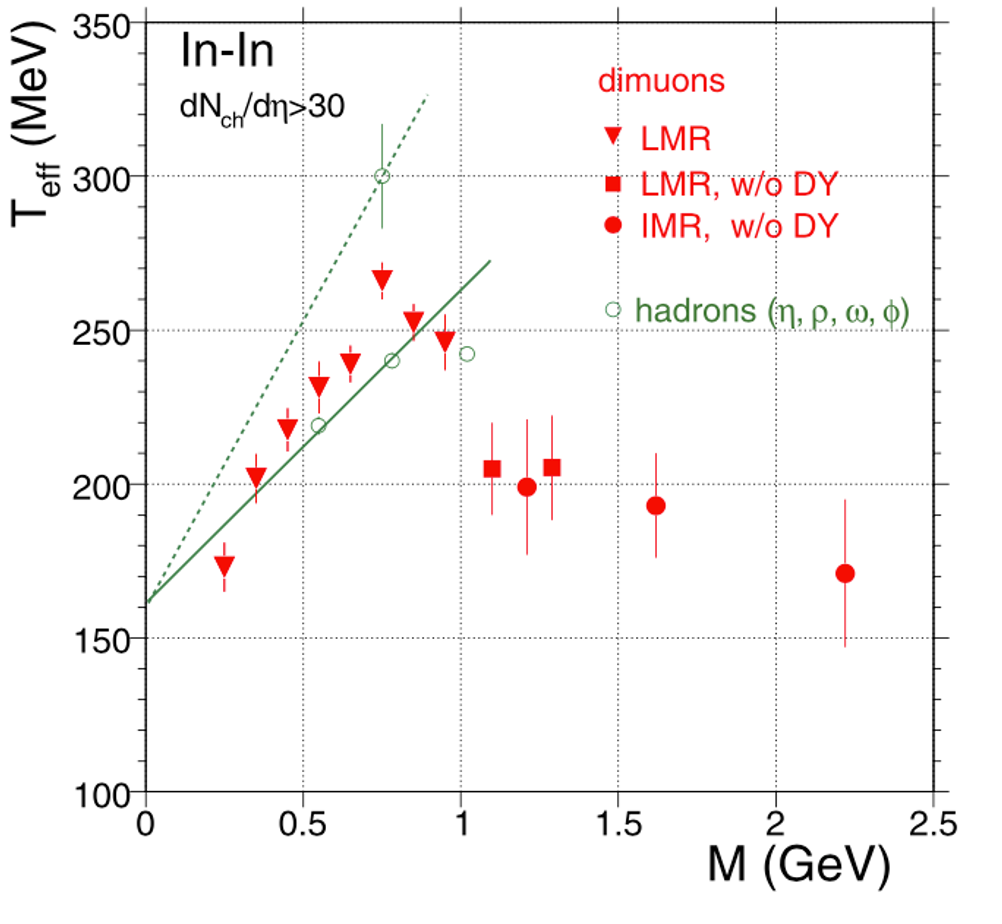
\includegraphics[width=0.75\textwidth,clip]{figures/Chapter1/NA60T.png}
    \end{center}
    \caption[NA60不同质量区间的有效温度测量结果]{NA60实验在不同质量区间下用$exp(-m_{T}/T_{eff})$拟合$m_T$谱得到的有效温度参数结果,并且与从强子谱得到的结果(绿色空心点)进行比较}
    \label{fig:NA60T}
\end{figure}

\subsubsection{PHENIX实验}

在RHIC上的双轻子测量主要由PHENIX(The Pioneering High Energy Nuclear Interaction eXperiment, PHENIX)实验和STAR(Solenoidal Tracker at RHIC)实验完成。

首先我们对PHENIX实验的双轻子测量结果进行一个简要的回顾。PHENIX实验是RHIC的两个大型粒子物理实验之一,其可以对中等快度区间内一定方位角的粒子进行测量,其探测器设计参数见参考文献[]。PHENIX首先对\sNN = 200 GeV质子-质子对撞中的双电子谱进行了测量,结果如图 \ref{fig:PHENIXpp} 所示。数据和强子衰变模拟的数据在误差范围内符合的很好,证明质子-质子对撞可以作为我们研究金-金对撞中的双电子谱时的基线。随后PHENIX也对 \sNN = 200 GeV 金-金对撞中的双电子谱进行了测量。在不同中心度下的结果如图 \ref{fig:PHENIXAuAu} 所示。在相对中心的对撞中心度下均观察到了在低质量区间($ 0.15 < M_{ee} < 0.75~{\rm GeV/c^2}$)相比于强子衰变模拟的产额增强。从图中也可以看到随着对撞接近中心对撞,这种产额增强的程度越来越高。这种增强和之前的预期相符。同时在低质量区间($M_{ee} < 0.3~{\rm GeV/c^2}$)和相对较高的横动量区间($ 1 < p_T < 5 ~{\rm GeV/c^2}$)的区间在质子-质子和金-金对撞中都观测到了产额的增强,在这个区间内的额外产额和质量的依赖关系和直生虚光子的产生的预测相符合。PHENIX也对直生虚光子进行了测量,但在本文中不进行详细的讨论,可参见参考文献[]。

\begin{figure}[htb]
    \centering
    \begin{subfigure}[b]{0.45\textwidth}
        \centering
        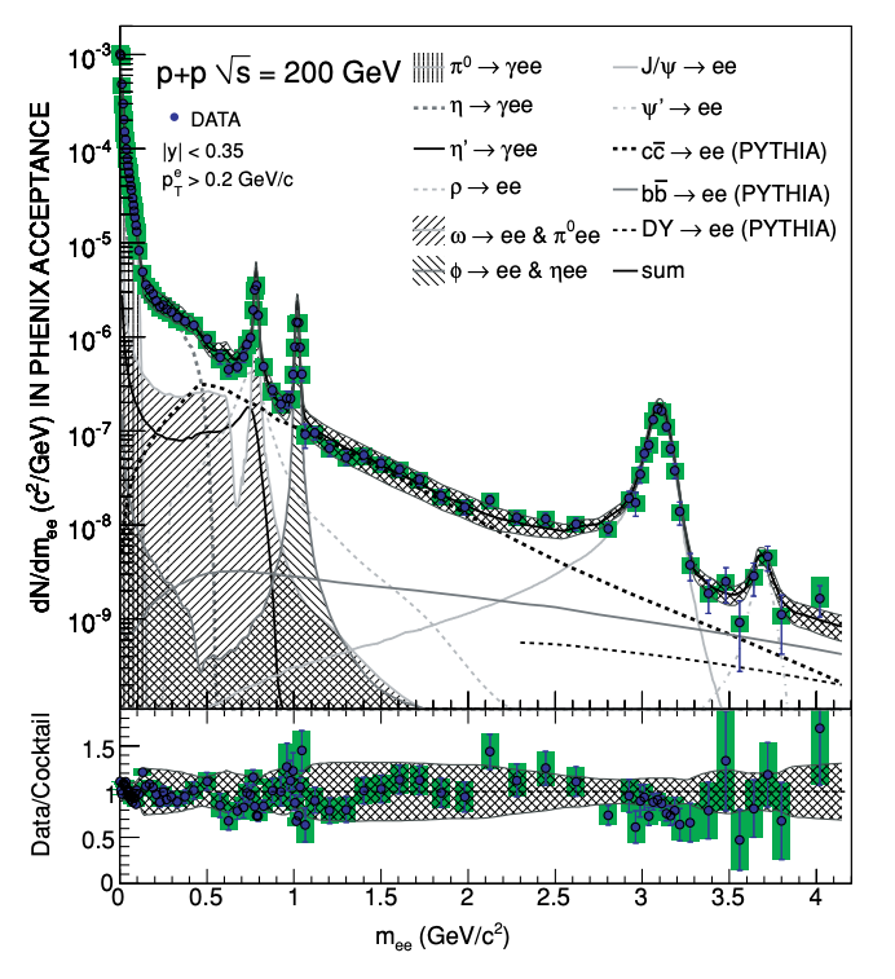
\includegraphics[width=\textwidth,clip]{figures/Chapter1/PHENIXpp.png}
        \caption{}
        \label{fig:PHENIXpp}
    \end{subfigure}
    \hfill
    \begin{subfigure}[b]{0.45\textwidth}
        \centering
        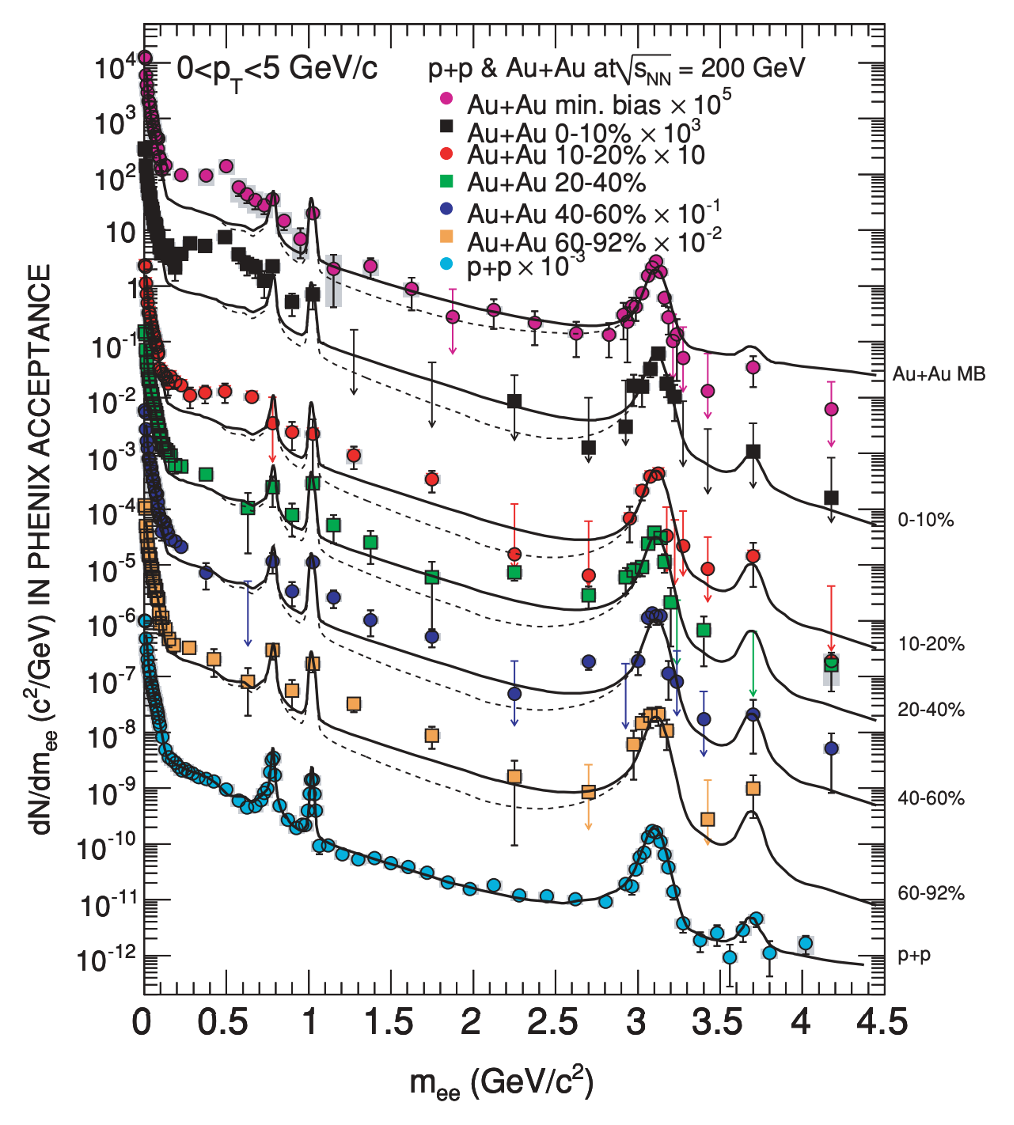
\includegraphics[width=\textwidth,clip]{figures/Chapter1/PHENIXAuAu.png}
        \caption{}
        \label{fig:PHENIXAuAu}
    \end{subfigure}
    \caption[PHENIX实验 \sNN = 200 GeV 质子-质子和金-金对撞中的双电子谱测量结果]{PHENIX实验在其接收度下的 \sNN = 200 GeV 质子-质子和金-金对撞中的双电子谱测量结果。左图为质子-质子对撞中的双电子谱测量结果。测量结果与强子衰变模拟的结果进行比较,强子衰变模拟的不同双电子源在图中已经标出。右图为\sNN = 200 GeV质子-质子和金-金对撞中不同中心度下的双电子谱。}
       \label{fig:PHENIXDiElectron}
\end{figure}

\subsubsection{STAR实验}

作为RHIC上的另一个大型粒子物理实验,STAR实验也对不同对撞系统和不同对撞能量中的双轻子谱进行了测量。在STAR的主径迹探测器时间投影室(Time Projection Chamber, TPC)和飞行时间探测系统(Time of Flight, TOF)的帮助下,STAR有能力获得高电子纯度的数据样本。以金-金 \sNN = 200 GeV 对撞的数据为例,其可获得电子纯度最高为94.6 ± 2 \%的数据样本。

和PHEINX实验类似,为了给离子-离子对撞中的测量定下一条好的基线,STAR的双轻子测量也是从质子-质子对撞开始的。STAR的首个双轻子测量结果基于2009年采集的质子-质子对撞数据,结果如图 \ref{fig:STARpp}所示。和PHENIX饰演的结果类似,强子衰变模拟也可以很好的描述测量到的双轻子谱。其中源自c夸克双电子模拟结果由PYTHIA6模拟得到。之后STAR合并2010和2011年两年的金-金 \sNN = 200 GeV下的数据进行了双电子谱的测量,如图 \ref{fig:STARAuAu}所示。在 $\rho$ 的质量区间($0.3 < M_{ee} < 0.76 ~{\rm GeV/c^2}$)STAR观测到了相比于强子衰变模拟1.76 ± 0.06 (stat) ± 0.26 (systematic) ± 0.29 (cocktail)倍的产额增强。STAR在 \sNNerbai 金金对撞中的测量结果在统计误差范围内和PHENIX合作组的测量结果可以符合,并且对于额外产额也和几种不同的理论模型进行了比较。

\begin{figure}[htb]
    \centering
    \begin{subfigure}[b]{0.43\textwidth}
        \centering
        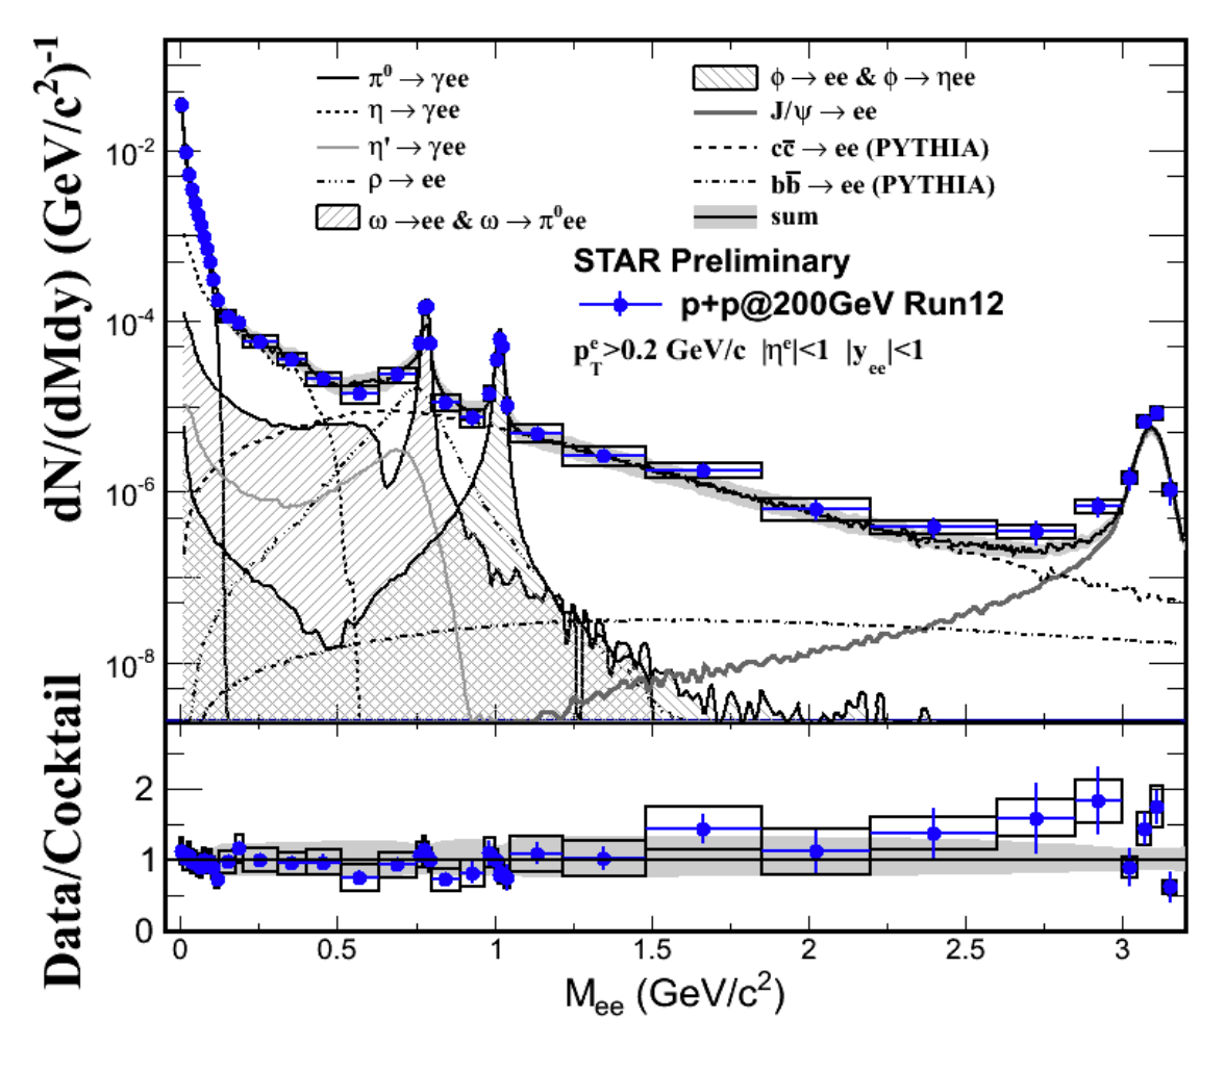
\includegraphics[width=\textwidth,clip]{figures/Chapter1/STARpp.png}
        \caption{}
        \label{fig:STARpp}
    \end{subfigure}
    \hfill
    \begin{subfigure}[b]{0.43\textwidth}
        \centering
        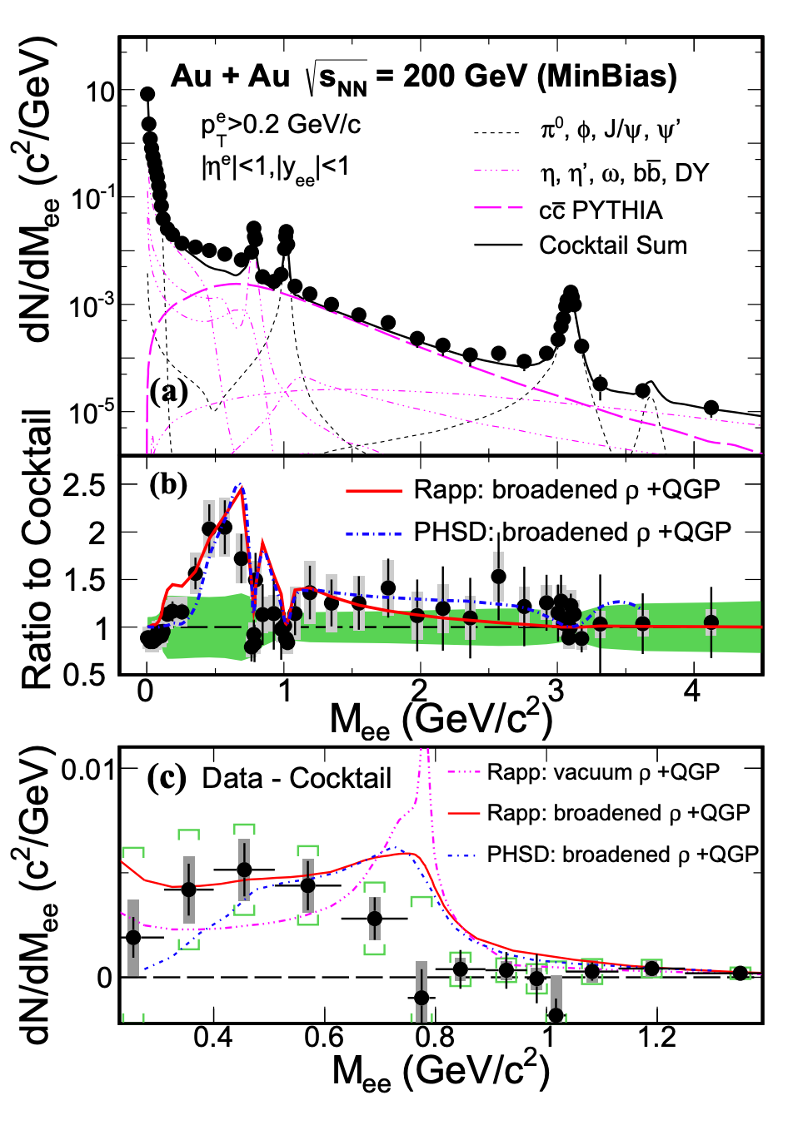
\includegraphics[width=\textwidth,clip]{figures/Chapter1/STARAuAu200.png}
        \caption{}
        \label{fig:STARAuAu}
    \end{subfigure}
    \caption[STAR实验 \sNN = 200 GeV 质子-质子和金-金对撞中的双电子谱测量结果]{STAR实验在其接收度下的 \sNN = 200 GeV 质子-质子和金-金对撞中的双电子谱测量结果。左图为质子-质子对撞中的双电子谱测量结果。测量结果与强子衰变模拟的结果进行比较,强子衰变模拟的不同双电子源在图中已经标出。右图的(a)部分为\sNN = 200 金-金对撞中0-80\%中心度下的双电子谱和强子衰变模拟的结果。(b)部分为数据和强子衰变模拟的比值,(c)部分为额外产额(data-cocktail),并且和几种不同的理论模型相比较}
       \label{fig:STARDiElectron}
\end{figure}

随着能量扫描(Beam Energy Scan)的进行,STAR在多个能量下对金-金对撞中的双电子谱进行了系统的测量。图展示了STAR在 \egyfive 金-金对撞中 0-80\%中心度下的双电子谱。在多个能量下STAR都观测到了在 $\rho$ 质量区间的产额增强。同时STAR在 \sNN = 19.6 GeV的金-金对撞中经过$dN_{ch}/d\eta$归一化和STAR接收度修正后额外产额和 NA60 \sNN = 17.3 GeV 铟-铟对撞下的额外产额可以很好的符合,结果见图 \ref{fig:STAR19p6}。理论模型也可以很好的描述\sNN = 19.6 GeV下双轻子额外产额。

\begin{figure}[htb]
    \begin{center}
    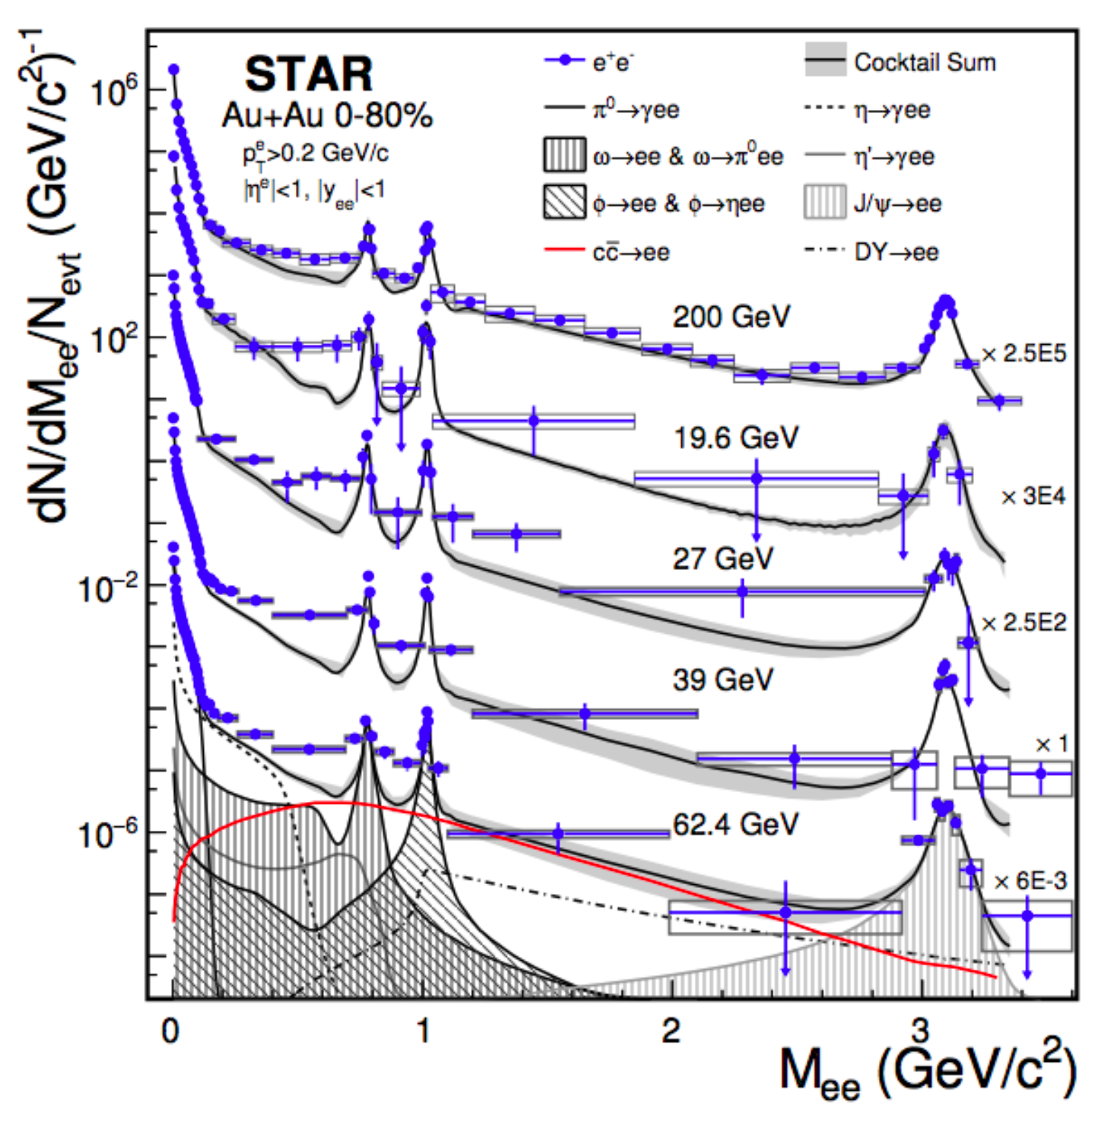
\includegraphics[width=0.6\textwidth,clip]{figures/Chapter1/STARBES.png}
    \end{center}
    \caption[STAR实验 \egyfive 下的双轻子谱]{STAR实验 \sNN = 19.6,27,39,62.4和200GeV下的双轻子谱。系统误差和统计误差分别用方框和竖线列出。图中仅展示了 \sNN = 62.4 GeV的强子衰变模拟结果,其余结果均与各自能量下的强子衰变模拟结果进行比较。}
    \label{fig:STARBES}
\end{figure}

\begin{figure}[htb]
    \begin{center}
    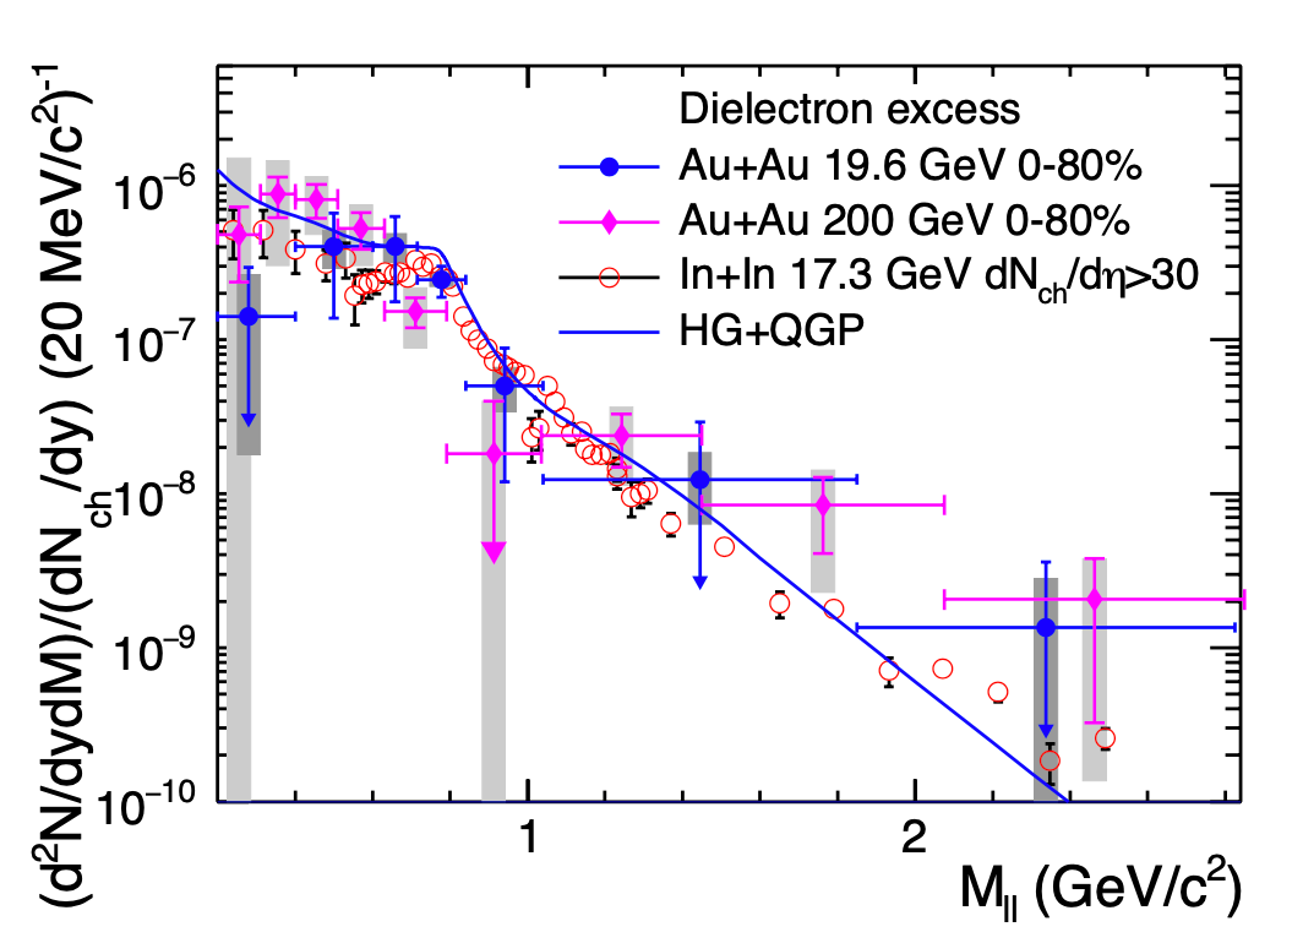
\includegraphics[width=0.6\textwidth,clip]{figures/Chapter1/STAR19p6.png}
    \end{center}
    \caption[STAR实验 \sNN = 19.6和200 GeV 的双轻子谱额外产额和NA60的额外产额比较]{STAR实验 \sNN = 19.6和200 GeV 的双轻子谱额外产额在经过中间快度区间的带电粒子多重数归一化和STAR接收度修正后和NA60的额外产额比较。蓝色实线为包含强子气(Hadron Gas)中broaden $\rho$ 和 QGP热辐射贡献的模型计算结果。 }
    \label{fig:STAR19p6}
\end{figure}

在 \sNN = 200GeV 的情况下,虽然有很高的统计但是随着对撞能量的增加,来源于重味夸克的双轻子在中等质量区间所占的产额比例逐渐增加,导致STAR在\sNN = 200GeV 双轻子测量中难以去抽取来自夸克胶子等离子体的热辐射产额。而在 \sNN = 19.6, 27, 39, 62.4 GeV 几个对撞能量下,虽然重味夸克的截面相比于\sNN = 200GeV 有所降低,但受限于统计也无法在中等质量区间进行热辐射产额的抽取。2017年STAR采集了大约12亿个\sNN = 54.4 GeV的金-金对撞事例。使得STAR有足够的统计在较低的对撞能量下尝试抽取来自于热辐射的双轻子产额。






 \cleardoublepage % each chapter begin with an odd number


\setcounter{section}{0}
%==========================================

%\section*{第一章:相对论重离子碰撞}


\setcounter{figure}{0}
\setcounter{table}{0}
\setcounter{equation}{0}




% \chapter{实验装置} \vskip -0.5cm
\chapter{实验装置}
% To add a non numbered chapter
%\addcontentsline{toc}{第一章}{相对论重离子碰撞}
% To insert this section on the table of contents
本文中所提到的分析和探测器升级都是基于相对论重离子对撞机(Relative Heavy Ion Collider, RHIC)上的STAR(Solenoidal Tracker at RHIC)实验。在接下来的一章中将会对RHIC和STAR实验进行简要的介绍,并对论文工作中所涉及的探测器进行简要的介绍。
\section{相对论重离子对撞机——RHIC}

相对论重离子对撞机位于美国纽约长岛上的布鲁克海文国家实验室(Brookhaven National Laboratory, BNL)内,
可以进行质心系能量最高为 \sNNerbai 的重离子对撞和质心系能量最高为 $\sqrt{s_{\mathrm{NN}}} = $ 510 GeV的极化质子-质子对撞。

相对论重离子对撞机是世界上第一台可以进行重离子对撞的对撞机,也是现存的唯一一台可以进行极化质子-质子对撞的对撞机。在RHIC上可以进行多种离子的对撞,以金-金对撞为例,其质心系能量最高可以达到 \sNNerbai 。对重离子对撞来说,因为RHIC具有可对撞离子种类多和能量范围宽的特点,可以进行多种离子系统和束流能量扫描,对研究夸克胶子等离子体的性质有着很大的帮助。

RHIC主要由两条独立的长约3.8公里(2.4英里)的加速储存环构成,离子或者质子可以在其中被加速到接近光速,并且在两个环的交叉点发生头对头碰撞。在整个RHIC环上两个环一共有6个交叉点可以来进行束流的头对头碰撞,束流在两条环里的运行方向相反,RHIC上的各个实验就位于这些交叉点的位置。离子或者质子在两个环当中以束流(Beam)的形式存在。其中沿着顺时针方向运行的束流被称作Blue Beam,沿逆时针方向运行的束流被称作Yellow Beam。从RHIC建成至今,一共有过STAR,PHENIX,PHOBOS 和 BRAHMS四个实验,分别位于RHIC环的 6点,8点,10点,和 2点钟方向。截止到本文写作时间(2022年)RHIC上仅有STAR实验还在运行取数,而RHIC也即将在不久的将来停机升级成电子-离子对撞机(e-RHIC)。

RHIC综合装置的示意图如图 \ref{fig:RHIC} 所示。接下来将以金离子为例介绍RHIC的离子加速过程。整个离子加速过程由三部分组成,金原子在经历整个过程后外层电子被剥离并被加速到所需要的束流能量
\begin{figure}[htb]
    \begin{center}
    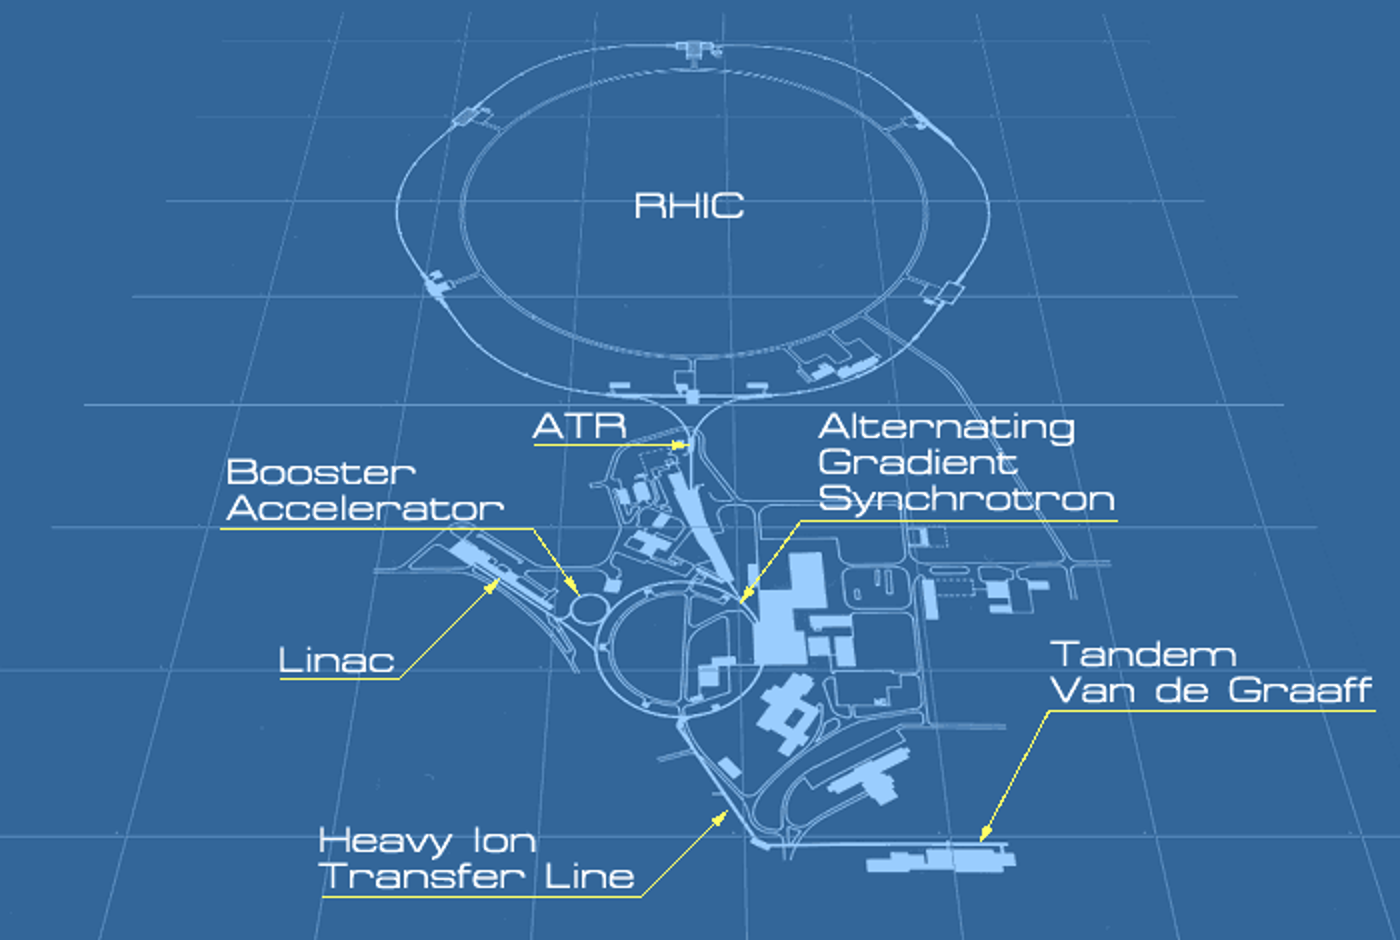
\includegraphics[width=0.8\textwidth,clip]{figures/Chapter2/RHIC.png}
    \end{center}
    \caption[相对论重离子对撞机(RHIC)综合装置示意图]{相对论重离子对撞机(RHIC)综合装置示意图}
    \label{fig:RHIC}
\end{figure}

金离子由脉冲溅射离子源(Pulser Sputter Ion Source)产生,带负电荷的金离子在串列范德格拉夫加速器(Tandem Van de Graaff)中被剥离一部分电子,变成电荷量为+32的金离子并被加速到 1MeV/$\mu$。之后电荷量为+32的金离子经过传输线被输送到增强器(Booster Synchrotron)中,在增强器中金离子被加速到 95 MeV/$\mu$ 并且外层电子被进一步剥离变成电荷量为+77的金离子并被注入到交变梯度同步加速器(Alternating Gradient Synchrotron, AGS)当中进行进一步的加速。电荷量为+77的金离子在交变梯度同步加速器被加速达到RHIC的注入能量 10.8 MeV/$\mu$后被送入AGS至RHIC的束流转移线(AGS-to-RHIC Beam Transfer Line)。金离子在束流转移线当中被剥离掉最后的电子成为电荷量为+79的离子后注入到RHIC当中,最后在RHIC中加速到对撞所需要的束流能量。
\section{RHIC上的螺线管径迹探测器——STAR}
RHIC上的螺线管径迹探测器(Solenoidal Tracker at RHIC,STAR)是坐落于RHIC 6点钟方向的大型粒子物理实验装置。在设计之初STAR就被赋予了丰富的物理目标,用以研究相对论重离子对撞产生的介质以及核子结构。整个探测器由多个子探测器组成,可以在高带电粒子多重数(RefMult)的环境下对末态粒子的径迹、动量、种类、能量等信息进行测量。在中心快度区间 ($|\eta| < 1 $),STAR具有全方位角 ($ 0 < \phi < 2\pi$)的接收度。STAR的核心径迹探测器为时间投影室(Time Projection Chamber, TPC),其可以对带电粒子的径迹进行测量并且通过电离能损信息($ \langle dE/dx \rangle $ )来进行粒子鉴别。

本文中的工作主要涉及以下子探测器:时间投影室,飞行时间探测器(Time of Flight, TOF),顶点位置探测器(Vertex Position Detector, VPD)以及STAR前向升级当中的小气隙板室(small-strip Tiny Gap Chamber, sTGC)。接下来的几个小节中将会对这些探测器进行简要的介绍。

\subsection{时间投影室}
\label{chap:TPC}
时间投影室是STAR最为核心的探测器也是STAR主要的径迹探测器。它可以提供穿过时间投影室的带电粒子的径迹和电离能损信息,并且通过这些信息计算径迹对应的粒子的动量和进行粒子鉴别。

其结构如图 \ref{fig:TPC} 所示。整个时间投影室为长4.2米,半径为2米的筒状结构。外部被一个大型螺线管磁铁环绕,用以提供沿着束流方向的匀强磁场。桶部为工作气体为P10 (10\%甲烷与90\%的混合气体)的漂移区,漂移区中心为内场膜,可以提供约为 135V/cm 的匀强电场。在端盖处为基于多丝正比室(Multi-Wire Proportional Chambers, MWPC)的读出系统。整个端盖处被分为了12 $\times$ 2个扇区,每个扇区为一个独立的多丝正比室。一个扇区的结构如图\ref{fig:MWPC}所示
\begin{figure}[htb]
    \begin{center}
    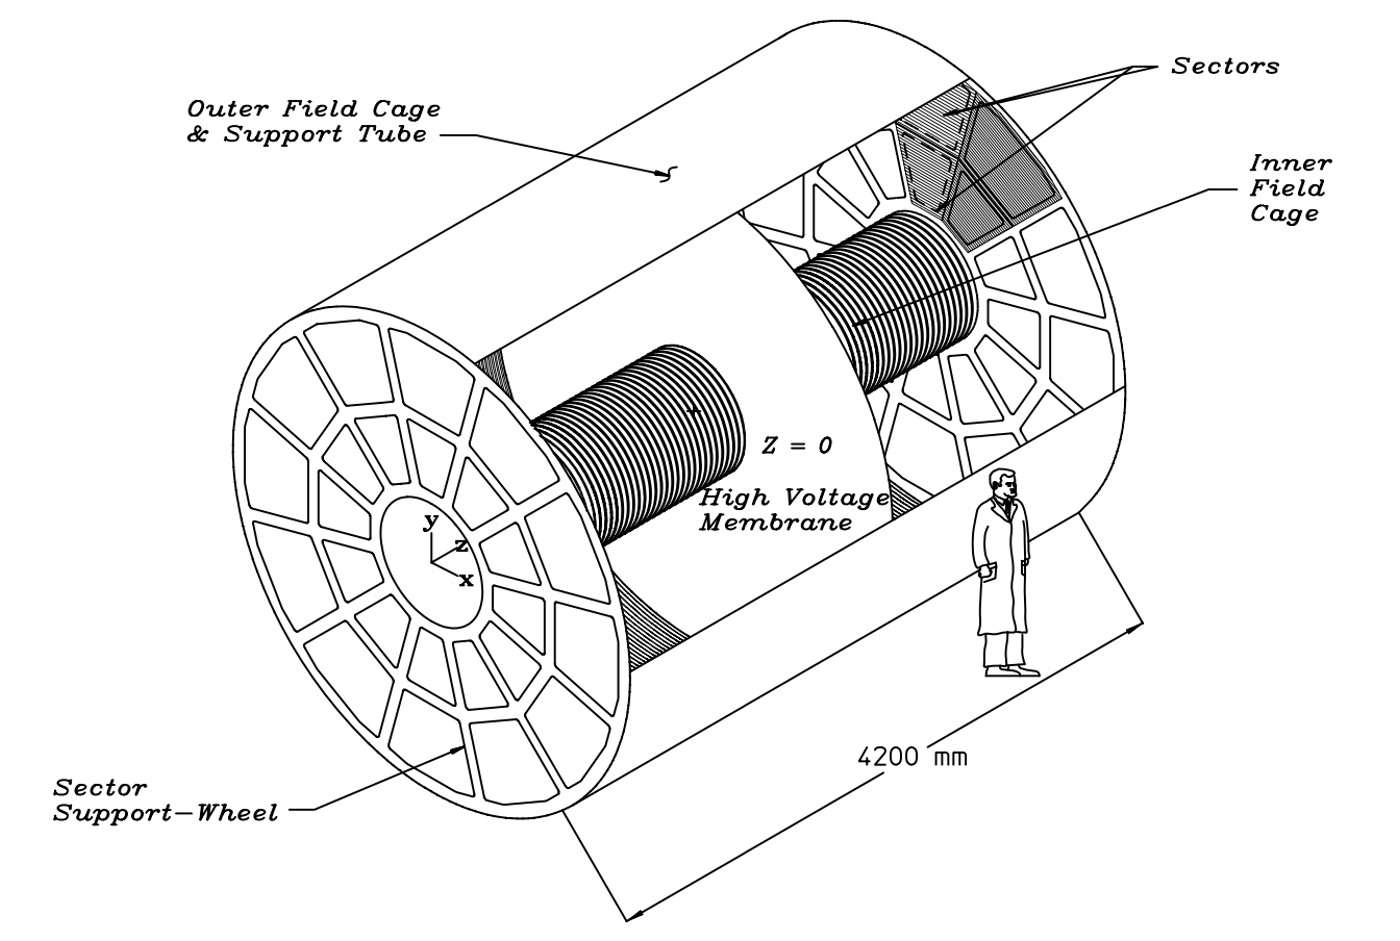
\includegraphics[width=0.75\textwidth,clip]{figures/Chapter2/TPC.png}
    \end{center}
    \caption[TPC结构示意图]{TPC结构示意图}
    \label{fig:TPC}
\end{figure}

图 \ref{fig:TPC_sector} 为时间投影室在2019年之前的扇区示意图,其中pad板排列密集的扇区为外扇区(outer sector),pad板排列稀疏的扇区为内扇区(inner sector)。从图中可以看到,内扇区的pad板排列明显稀疏于外扇区,粒子在穿过内扇区时最多留下13个击中(Hit)的信息用以径迹重建,这导致时间投影室在 $\eta$ 相对较大的范围的接收度变差。STAR于2019年进行了TPC内扇区(inner TPC, iTPC)的升级,对全部的内扇区进行替换升级,升级后的内扇区结构示意图见图 \ref{fig:iTPC} 。可以看到升级之后的内扇区的pad板密度明显增加。内扇区升级提高了整个时间投影室在大的$\eta$区间接收度、提升了时间投影室的径迹重建和粒子鉴别的能力并且使得时间投影室对低横动量的粒子的测量能力得到了进一步的提升。

\begin{figure}[htb]
    \centering
    \begin{subfigure}[b]{0.47\textwidth}
        \centering
        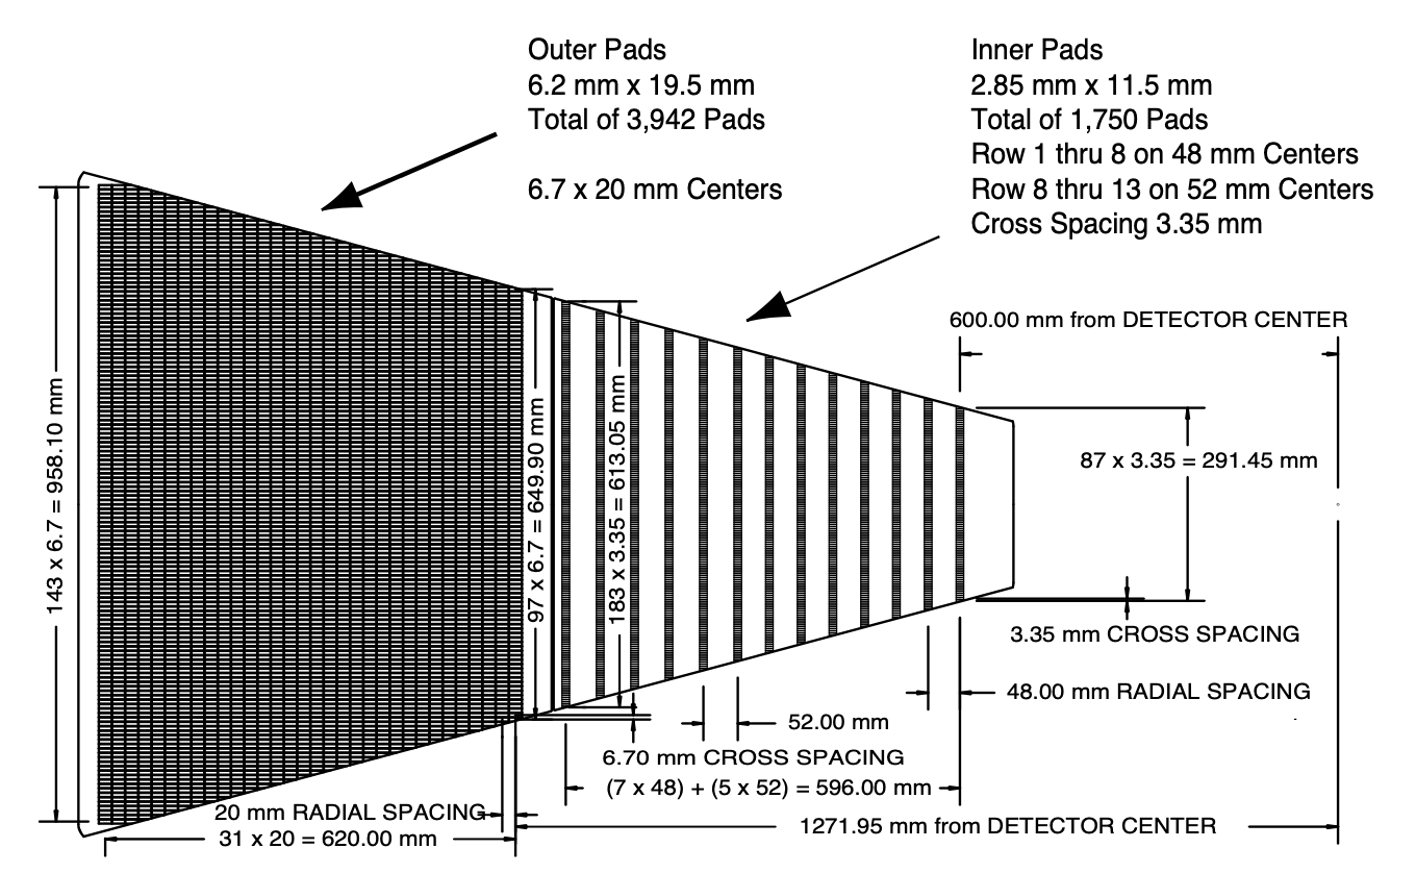
\includegraphics[width=\textwidth,clip]{figures/Chapter2/MWPC.png}
        \caption{}
        \label{fig:TPC_sector}
    \end{subfigure}
    \hfill
    \begin{subfigure}[b]{0.47\textwidth}
        \centering
        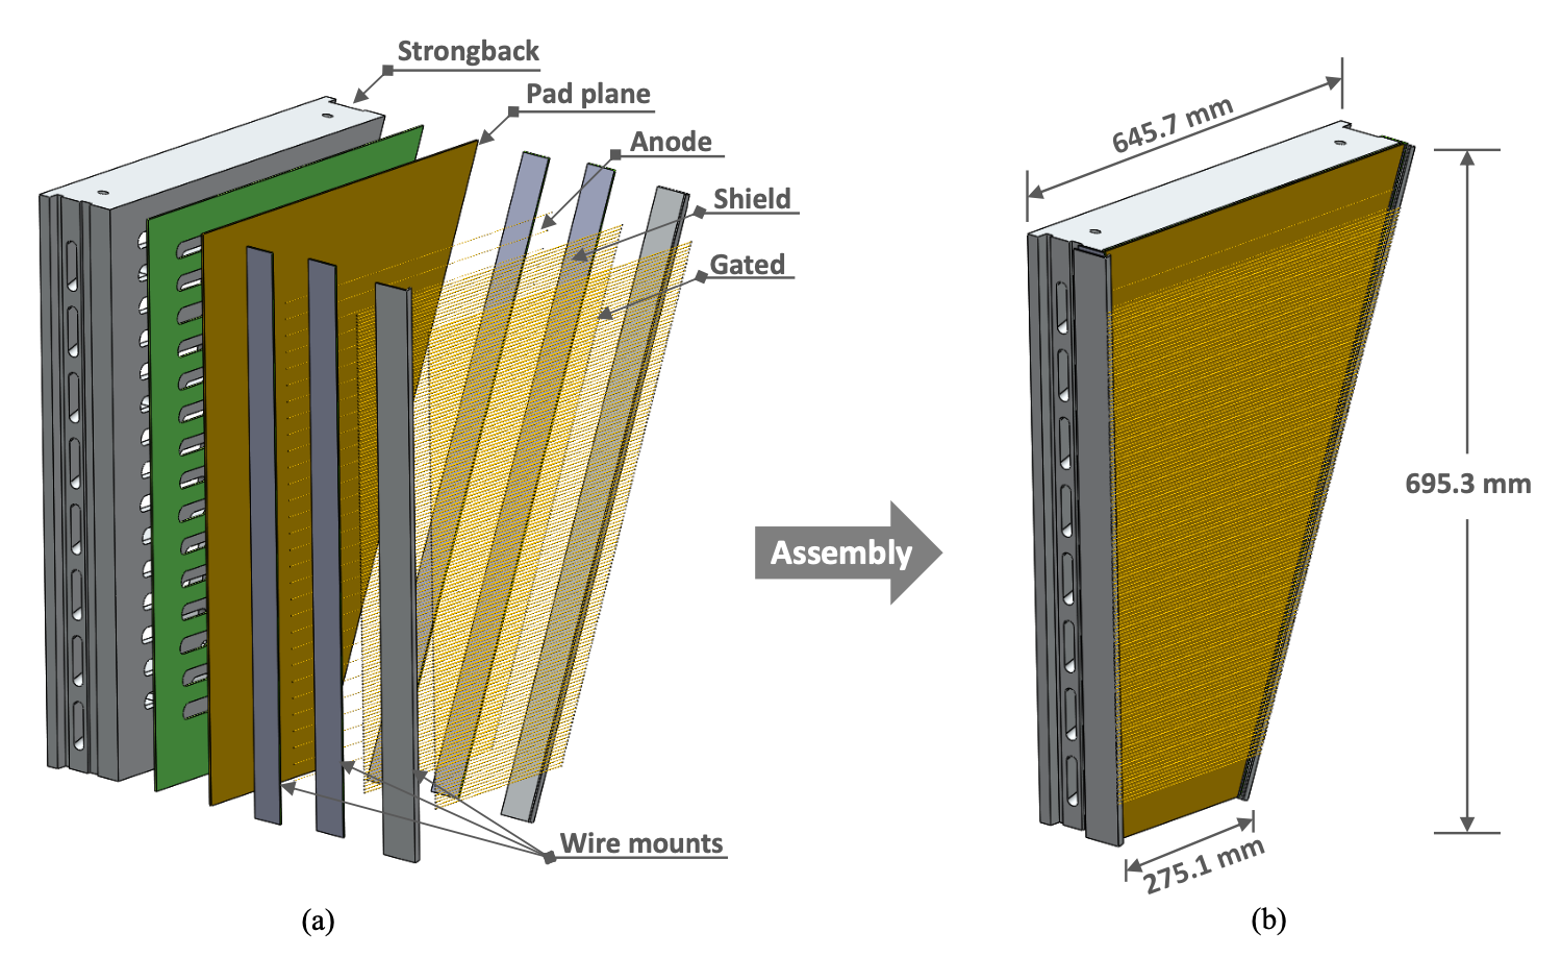
\includegraphics[width=\textwidth,clip]{figures/Chapter2/iTPC.png}
        \caption{}
        \label{fig:iTPC}
    \end{subfigure}
       \caption[TPC扇区示意图与iTPC升级后结构示意图]{图(a)为时间投影室升级之前一个扇区示意图,其中pad板排列密集的扇区为外扇区,pad板排列稀疏的扇区为内扇区。图(b)为升级后的内扇区结构示意图}
       \label{fig:MWPC}
\end{figure}

当带电粒子穿过时间投影室的时候,带电粒子会在匀强磁场的作用下发生偏转并且在漂移区的工作气体中电离产生原初电子-离子对,其中的电子在匀强电场的作用下向端盖处由多丝正比室组成的读出端漂移。因为P10气体的性质,电子在较低的电压下有着比较高的漂移速度。同时又因为时间投影室在漂移速度曲线的峰值附近工作,所以整个漂移速度受到气压和温度的影响较小,可以保持一个比较稳定的漂移速度。在STAR的取数过程中,也会每隔四个小时采集一个laser run来对时间投影室的漂移速度进行校正。
整个漂移过程中,电子束团(Cluster)的横向扩散约为 $\sigma_{T} = 3.3mm$ (漂移距离210cm),纵向(沿着漂移方向)扩散为$\sigma_{L} = 5.2mm$。对时间投影室来说,电子束团在横向和纵向的扩散会直接影响读出端丝室的设计。
当电子漂移到时间投影室的端盖处,电子会在通上高压的阳极丝附近发生雪崩过程,同时在阴极的pad板平面上产生感应信号,此感应信号被电子学采集之后通过电荷重心法可以确定出一个击中(Hit)的 X,Y 位置。因为整个漂移过程中漂移速度是稳定的,所以Z方向上的位置由漂移时间来决定。图\ref{fig:HowTPCWrok}展示了粒子在时间投影室中产生信号并被收集的过程。

\begin{figure}[htb]
    \begin{center}
    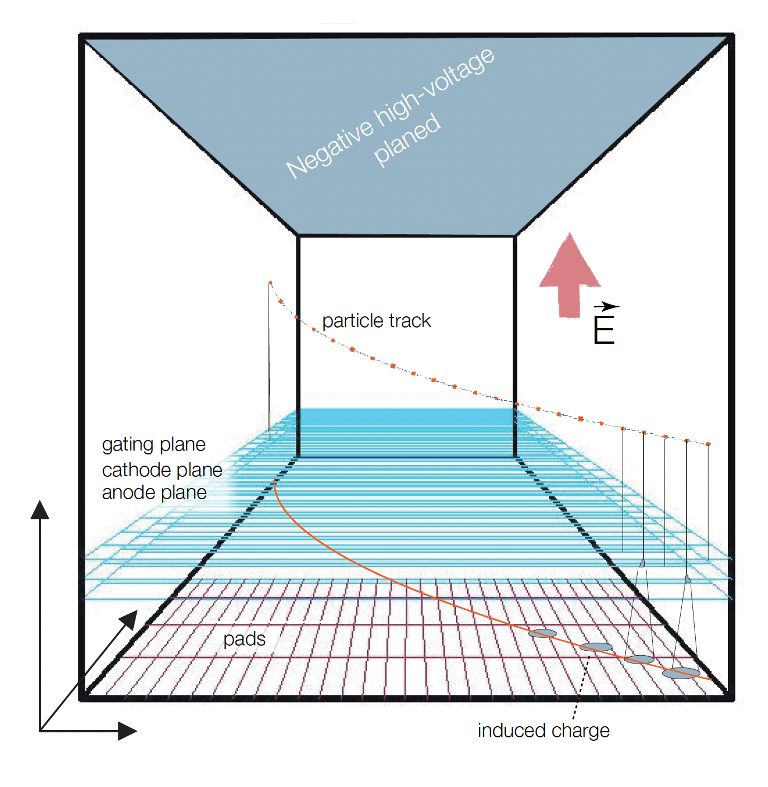
\includegraphics[width=0.75\textwidth,clip]{figures/Chapter2/HowTPCWork.png}
    \end{center}
    \caption[时间投影室工作原理示意图]{时间投影室工作原理示意图,展示了粒子在TPC中电离后产生的原初电离电子经由读出端丝室放大后在pad平面上产生感应信号的过程}
    \label{fig:HowTPCWrok}
\end{figure}

以上就是在时间投影室中带电粒子发生一次电离并且通过读出端收集到信号进行击中重建的大致过程。在一次对撞发生时会产生大量的末态的带电粒子,这些粒子在穿过漂移区的时候会发生多次电离,在读出端留下大量的击中信息。在收集到这些信号之后,需要通过算法将这些击中重建成径迹(Track)。

在时间投影室端盖处作为信号收集系统的多丝正比室工作在正比区,所以读出系统采集到的信号幅度大小和带电粒子在时间投影室中电离损失的能量成正比。当粒子在气体中电离时,其平均电离能损$ \langle dE/dx \rangle $可以通过Bethe-Bloch公式计算得到,公式如下:
\begin{equation}
    -\frac{dE}{dx} = 4\pi N_A r_c^2 m_e c^2 z^2\frac{Z}{A}\frac{1}{\beta} \bigg[ ln\frac{2 m_e c^2 \beta^2 \gamma^2 }{I} - \beta^2 - \frac{\delta}{2} \bigg ]
    \label{eq:BB}
\end{equation}

其中z为入射粒子电荷,Z为介质的原子序数,A为介质的原子量,$M_e$为电子质量,$r_c$是电子经典半径,$N_A$是阿伏伽德罗常数,I为介质的平均激发能,$\beta = v/c$为带电粒子的速度,$\delta$为描述入射的相对论性粒子的横向电场被原子电子电荷密度屏蔽程度的参数。需要注意的是,上式适用于入射粒子质量远大于电子质量的情形。当入射粒子为电子时,Bethe-Bloch公式可以近似为:
\begin{equation}
    -\frac{dE}{dx} = 4\pi N_A r_c^2 m_e c^2 \frac{Z}{A}\frac{1}{\beta} \bigg[ \frac{1}{2}ln\frac{m_e c^2 \gamma }{2I} - \beta^2 - \frac{\delta^*}{2} \bigg ]
\end{equation}
其中$\delta^*$与式 \ref{eq:BB} 中的$\delta$略有不同。图 \ref{fig:dEdx}为不同粒子在时间投影室中电离能损随动量变化的示意图,可以看到在相同的动量的时候不同粒子有着不同的电离能损,时间投影室就可以通过测量径迹的平均电离能损$ \langle dE/dx \rangle $的方式来进行粒子鉴别。同时可以看到在动量较高的区间电子和 $\mu$子,$\pi$介子的电离能损无法较好的分辨。我们需要额外的信息来帮助我们进行粒子鉴别,例如速度信息。粒子速度的测量将在下一小节中进行介绍

\begin{figure}[htb]
    \begin{center}
    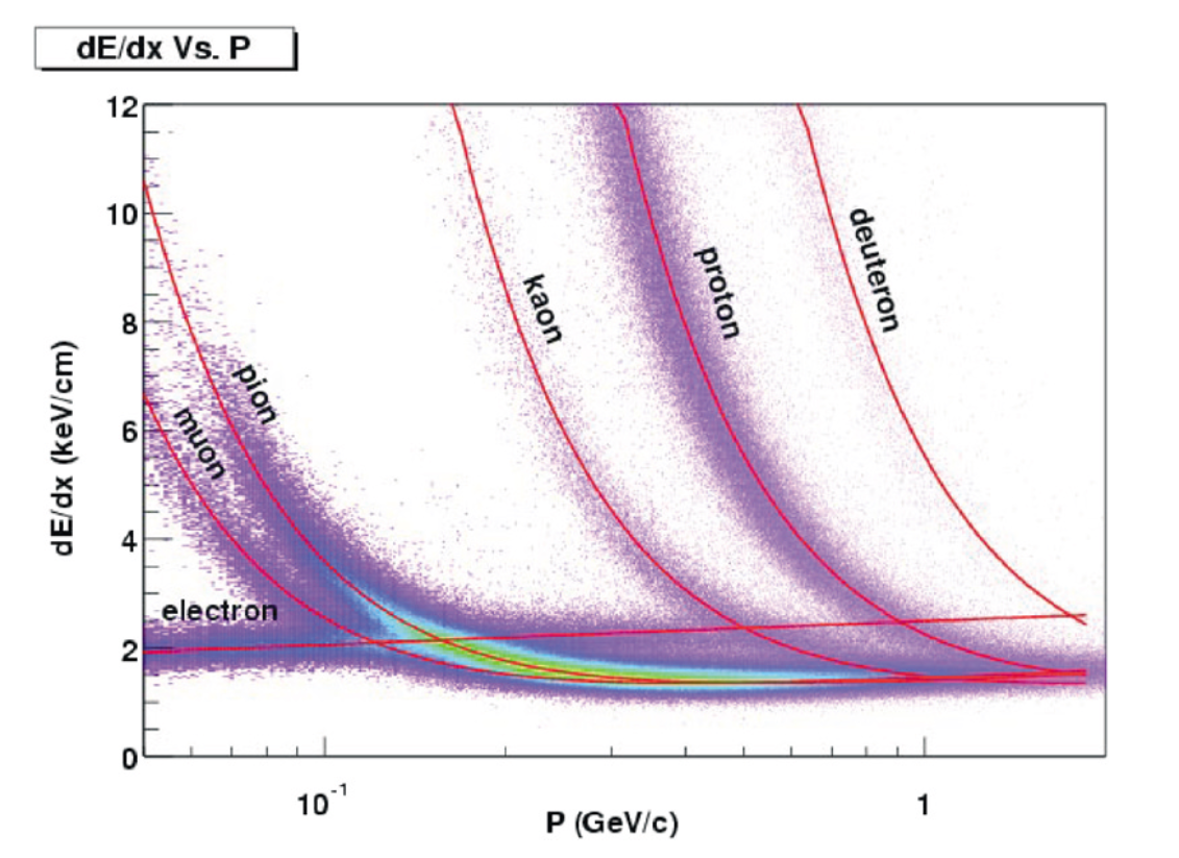
\includegraphics[width=0.75\textwidth,clip]{figures/Chapter2/dEdx.png}
    \end{center}
    \caption[粒子在时间投影室中的电离能损]{不同种类粒子在时间投影室中电离能损随着动量变化示意图。本图中数据在磁场为0.25T的环境下测量}
    \label{fig:dEdx}
\end{figure}

\subsection{飞行时间探测器}

如上小节中所讨论,在动量相对较高的区间我们需要额外的信息来帮助进行粒子鉴别。飞行时间探测器(Time of Flight, ToF)被设计用来测量粒子的飞行速度从而进行粒子鉴别。这就对TOF的性能提出了如下要求:
\begin{itemize}
    \item 时间分辨率小于100ps, 对于停止时间(Stop time)的测量,时间分辨率应小于80ps。
    \item 每个通道的响应时间快,从而可以在在高粒子多重数的环境下工作
    \item 可以在STAR的磁场环境(0.5T)下稳定工作
    \item 成本相对较低,可以覆盖较大的范围从而与TPC中的径迹进行配对,空间接收度应与TPC类似。
\end{itemize}

基于这这些需求,多气隙电阻板室(Multi-gap Resistive Plate Chamber, MRPC)被用来作为TOF的终止时间测量探测器,起始时间由顶点位置探测器(Vertex Position Detector, VPD)给出。多气隙电阻板室首先被应用在ALICE实验上的时间飞行探测器当中,有着很高的时间分辨率且可以在高粒子多重数、强磁场的环境下工作。图 \ref{fig:MRPC} 为STAR中多气隙电阻板室的结构示意图。
\begin{figure}[htb]
    \begin{center}
    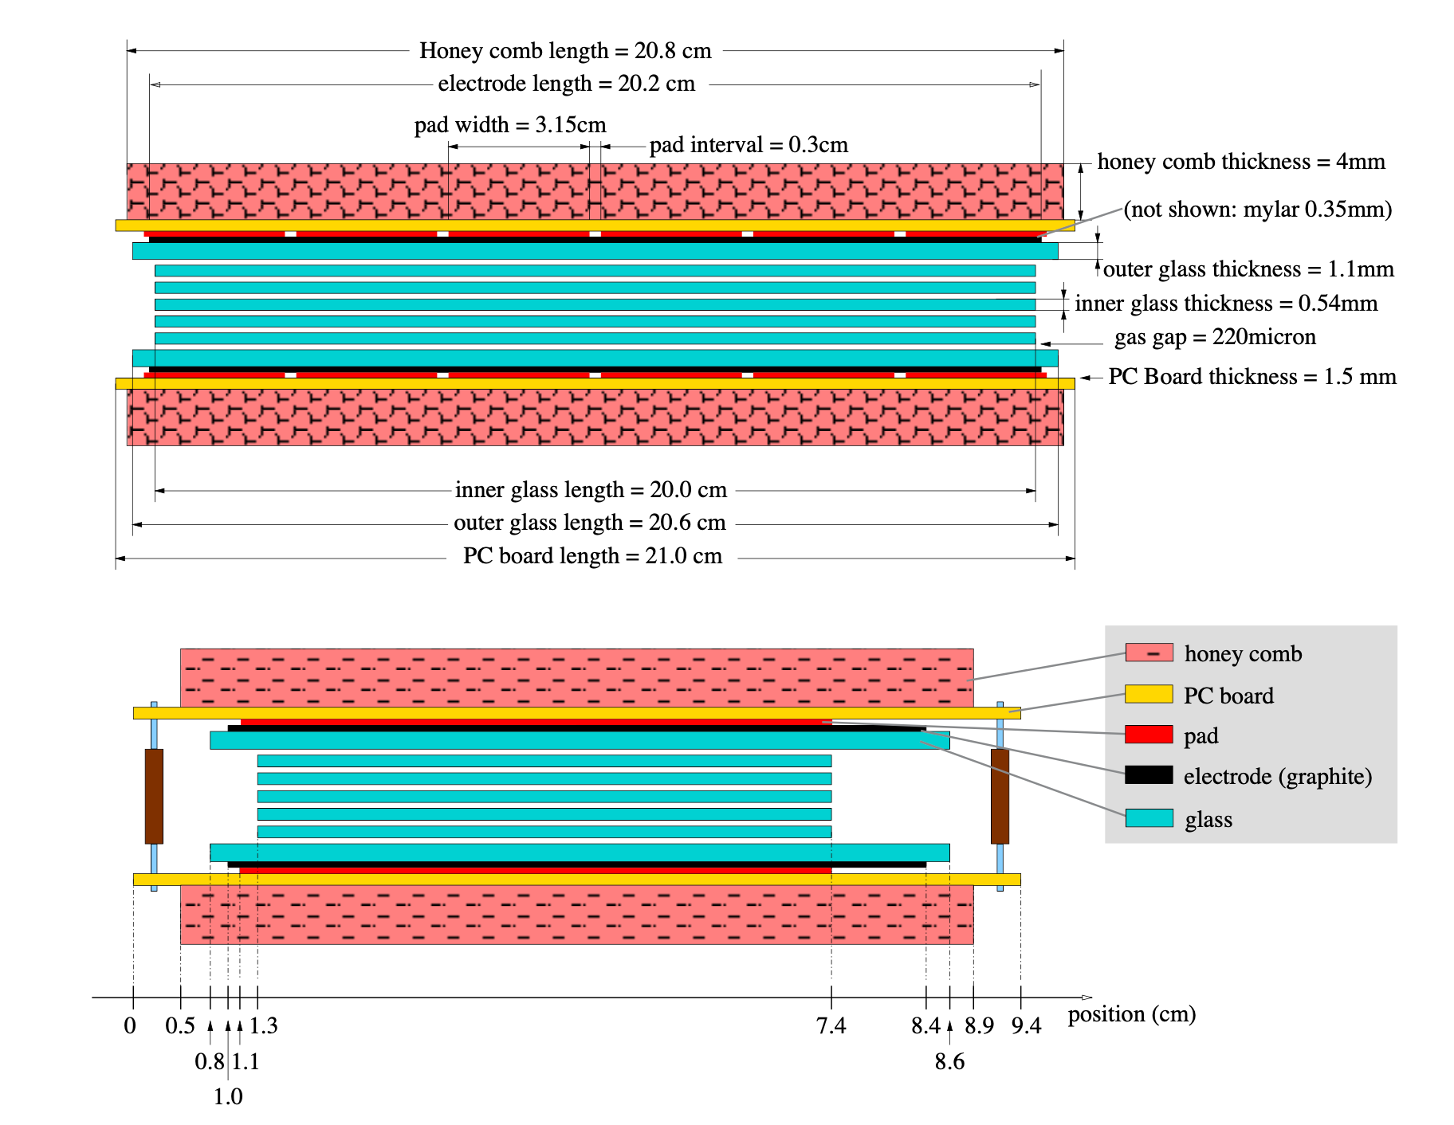
\includegraphics[width=0.7\textwidth,clip]{figures/Chapter2/MRPC.png}
    \end{center}
    \caption[MRPC结构示意图]{STAR上MRPC的测试图,上图为沿长边方向,下图为沿短边方向}
    \label{fig:MRPC}
\end{figure}
如图所示,在两个电极之间插入了5块阻性玻璃板,电极之间加有高压,可以在阻性板和阻性板之间的气隙之间产生高压。当带电粒子穿过整个室的时候可以在每个气隙处发生独立的雪崩过程。对于整个室而言,读出端所得到的感应信号相当于多个间隙内雪崩的“瞬时”叠加,因此可以获得一个相对较大的信号。多气隙电阻板室相对于传统的的阻性板室(Resistive Plate Chamber, RPC)计数率可以得到很大的提高。每个多气隙电阻板室具有6个 6.1 $\times$ 3.4cm 的读出pad,这使得飞行时间探测器的读出有着相对较好的读出粒度,使飞行时间探测器上的击中可以与时间投影室中的径迹进行配对。飞行时间探测器中的多气隙电阻板室的接收度和时间投影室类似,也有着全方位角($ 0 < \phi < 2\pi$)和中心快度区间($ |\eta| < 0.9 $)的接收度。

结合多气隙电阻板室测得的终止时间和顶点位置探测器测得的起始时间可以得到径迹的飞行时间,再利用时间投影室测量得到的径迹长度信息可以计算得到粒子的飞行速度用以进行粒子鉴别,图 \ref{fig:TOFPerformance} 展示了TOF测量的 $1/\beta$ 随动量变化的分布以及添加 $1/\beta$ 判选条件后的电离能损分布。可以看到,在额外添加$|1-1/\beta| < 0.03$的判选条件时,电子的电离能损可以很好的与其他粒子区分开来。整个STAR探测器的粒子鉴别能力在添加径迹的速度信息后得到了很好的提升。

\begin{figure}[htb]
    \centering
    \begin{subfigure}[b]{0.47\textwidth}
        \centering
        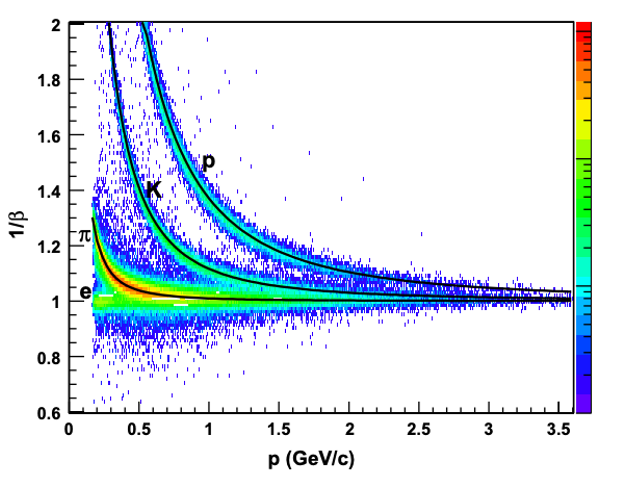
\includegraphics[width=0.9\textwidth,clip]{figures/Chapter2/BetaDistribution.png}
        \caption{}
        \label{fig:BetaDis}
    \end{subfigure}
    \hfill
    \begin{subfigure}[b]{0.47\textwidth}
        \centering
        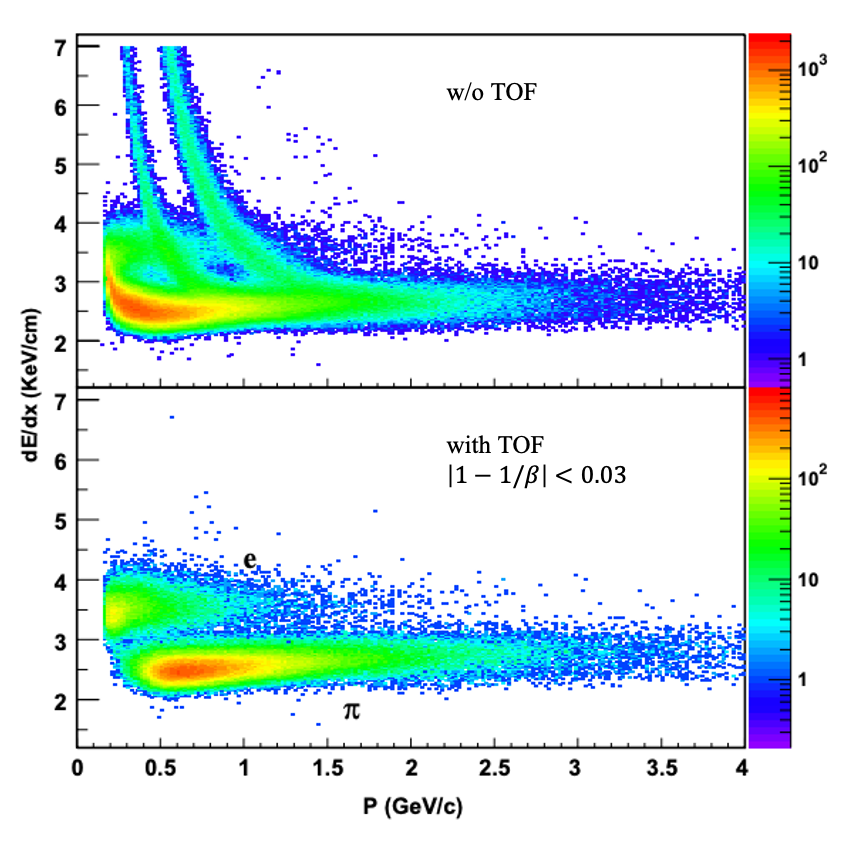
\includegraphics[width=0.9\textwidth,clip]{figures/Chapter2/dEdxwithTOF.png}
        \caption{}
        \label{fig:dEdxwithTOF}
    \end{subfigure}
       \caption[飞行时间探测器粒子鉴别表现]{图(a)粒子的$1/\beta$分布随着动量变化的示意图。图(b)为电离能损(dE/dx)随着动量变化的分布。上半部分为仅用时间投影室测量,不添加额外的关于$\beta$的判选条件的电离能损分布。下半部分为在上半部分基础上额外添加 $|1-1/\beta| < 0.03$的判选条件时的电离能损分布}
       \label{fig:TOFPerformance}
\end{figure}
  



 \cleardoublepage 
\setcounter{section}{0}
%==========================================

\setcounter{figure}{0}
\setcounter{table}{0}
\setcounter{equation}{0}

\chapter{STAR前向升级——STAR Forward Upgrade}

\section{STAR前向升级}

在过去二十余年的运行过程中,STAR采集了许多 p+p,p+A对撞的数据,并且基于这些数据在cold QCD领域得到了很好的测量结果。STAR的主要探测器集中在中心赝快度区域($|\eta| < 1$),
有关前向的物理测量较少,但不论对于cold QCD还是重离子对撞来说,前向方向都是一个十分令人感兴趣的区间。有着丰富的物理目标等着我们去探索。

在过去的二十年当中,STAR前向的测量任务主要由前向介子谱仪(Forward Meson Spectrometer, FMS)完成。
前向介子谱仪是一个安装在STAR西侧前向快度区间的电磁量能器,其由两种不同规格共计1264块铅玻璃构成。如图\ref{fig:FMS}所示。前向介子谱仪是一个全吸收型电磁量能器,铅玻璃可以同时充当能量沉积的载体和探测手段。
但对于电磁量能器来说,其主要鉴别电子的手段是通过计算E/p 的值从而进行电子鉴别。这就要求除了单独的一个量能器我们还需要有能力对打在探测器上的粒子进行径迹和动量的探测,所以我们希望前向除了量能器以外能额外的有径迹探测的手段。并且作为电磁量能器,前向介子谱仪并不能对$\pi^0$、中子、光子等中性粒子进行测量。

在近些年来STAR实验进行了一些升级,例如前文提到的iTPC升级以及新加装的事例平面探测器(Event Plane Detector, EPC)。但iTPC作为STAR主径迹探测器时间投影室的一部分,覆盖的赝快度区间仍然有限,不能覆盖 $|\eta| > 2$的范围。而事例平面探测器虽然可以覆盖较为前向(西侧)和背向(东侧)的赝快度范围($2.14 < |\eta| < 5.09 $),但其探测器每个最小探测单元粒度很大,且只有一层,无法进行径迹重建。如果同时可以扩展径迹探测器所覆盖的赝快度区间,STAR实验将有能力对极大或者极小的Bjorken x区间进行更多物理量的测量,有助于加深对cold QCD的理解。同时RHIC将于2025年开始进行升级成为电子-离子对撞机(Electron-Ion Collider, EIC)。在前向的物理测量和探测器升级可以为以后基于电子-离子对撞机的探测器建设起指导作用和积累经验。

基于这些需求,STAR提出了前向升级计划(Forward Upgrade),如图\ref{fig:FWD}所示,覆盖了$ 2.5 < \eta < 4 $的赝快度区间。整个前向升级由两部分构成:前向量能器系统(Forward Calorimeter Systerm, FCS)和前向径迹探测系统(Forward Tracking System, FTS)。其中前向量能器系统由电磁量能器(Electromagnetic Calorimeter, Ecal)和强子量能器(Hadronic Calorimeter, HCal)组成。前向电磁量能器为铅闪烁体取样量能器,前向强子量能器为三明治型铁闪烁体板取样型能器。前向电磁量能器和强子量能器都有着很好的能量分辨,电磁量能器能量分辨可达到~$8\%/\sqrt{E}$,强子量能器的能量分辨可以达到~$70\%/\sqrt{E}$。
\begin{figure}[htb]
    \begin{center}
    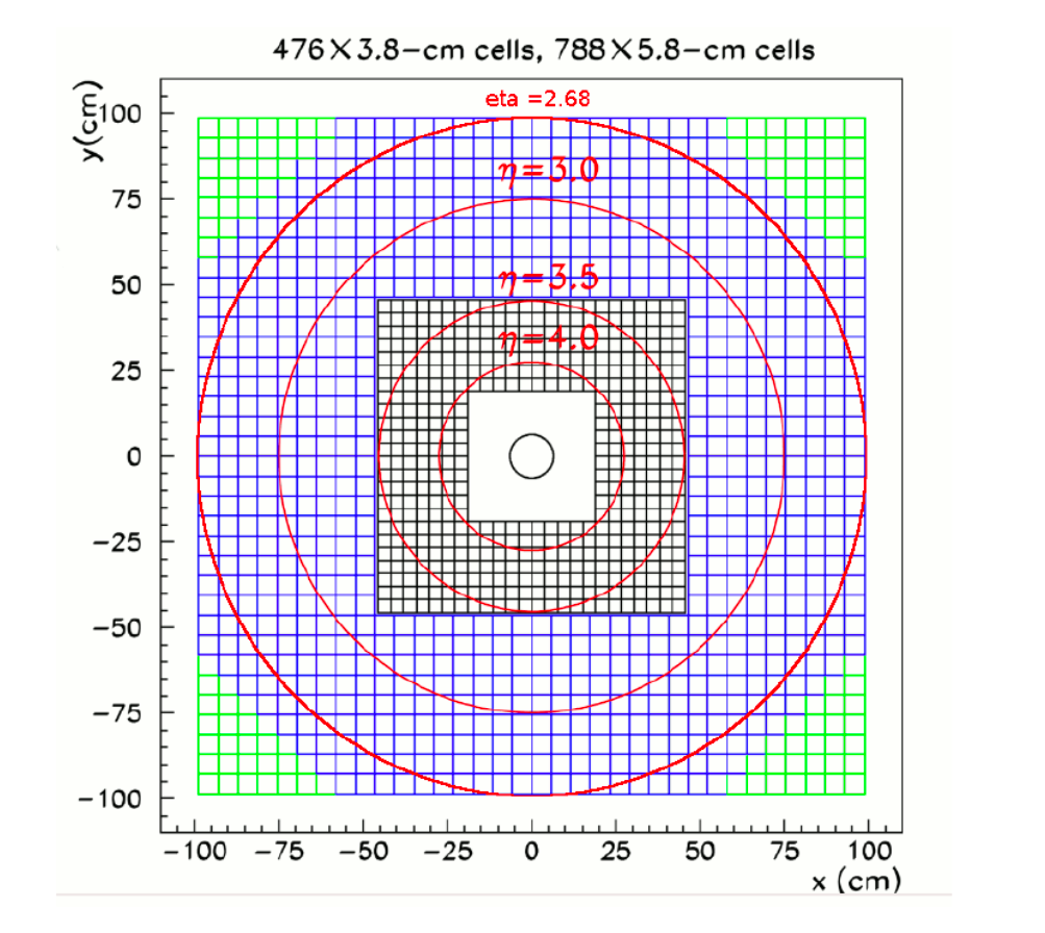
\includegraphics[width=0.8\textwidth,clip]{figures/Chapter3/FMS.png}
    \end{center}
    \caption[前向介子谱仪(FMS)示意图]{前向介子谱仪(FMS)示意图}
    \label{fig:FMS}
\end{figure}
\begin{figure}[htb]
    \begin{center}
    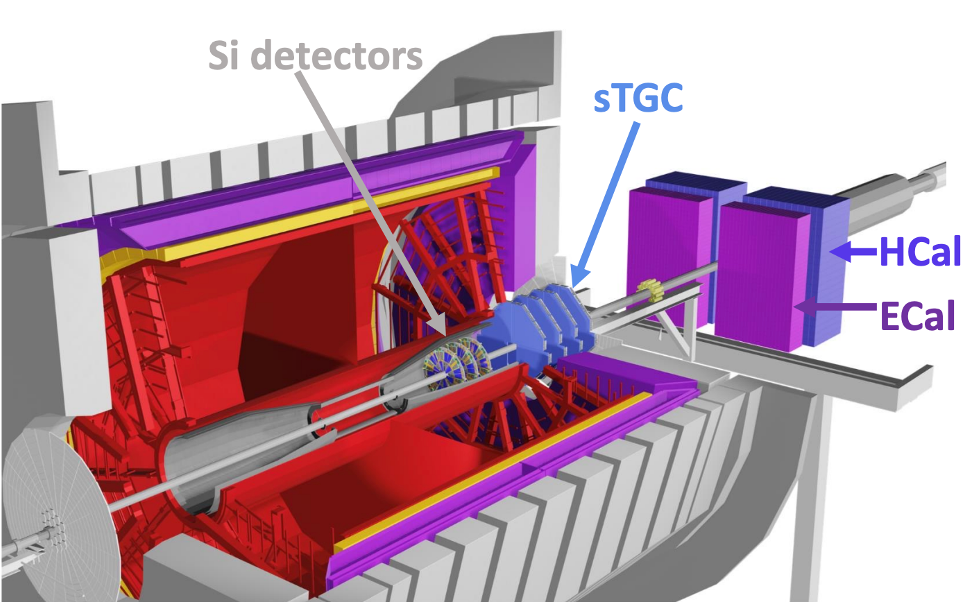
\includegraphics[width=0.8\textwidth,clip]{figures/Chapter3/FWD.png}
    \end{center}
    \caption[STAR前向升级示意图]{STAR前向升级示意图,各子探测器已在图上标出}
    \label{fig:FWD}
\end{figure}
前向硅径迹探测器(Forward Silicon Tracker, FST)和前向小气隙室径迹探测器(Forward sTGC Tracker, FTT)共同组成了STAR前向升级当中的前向径迹探测系统。

因为STAR在Run14-Run16期间曾经在对撞点(Interaction point)附近安装过重味粒子径迹探测器(Heavy Flavor Tracker, HFT),有过硅径迹探测器的安装操作经验,所以硅探测器被考虑用来作为前向径迹探测器的一部分。前向硅径迹探测器由三层圆盘状的硅探测器组成,覆盖$2\pi$的方位角和$2.5 < \eta < 4$的快度区间。作为径迹探测系统的一部分,前向硅径迹探测器可以为整个径迹系统提供三个点来进行径迹重建。

在过去的二十年间,窄隙室得到了长足的发展并被应用到了ATLAS实验前向New Small Wheel升级当中,技术已经相对成熟,有着成本低和物质的量小的优点,适合在离对撞点较远的位置用于径迹探测。整个前向小气隙室径迹探测器由四层sTGC平面组成,可以为径迹探测系统提供四个点用于径迹重建。对于每一个sTGC平面,其由四个五边形的模块拼接而成,如图 \ref{fig:sTGC} 所示。
\begin{figure}[htb]
    \begin{center}
    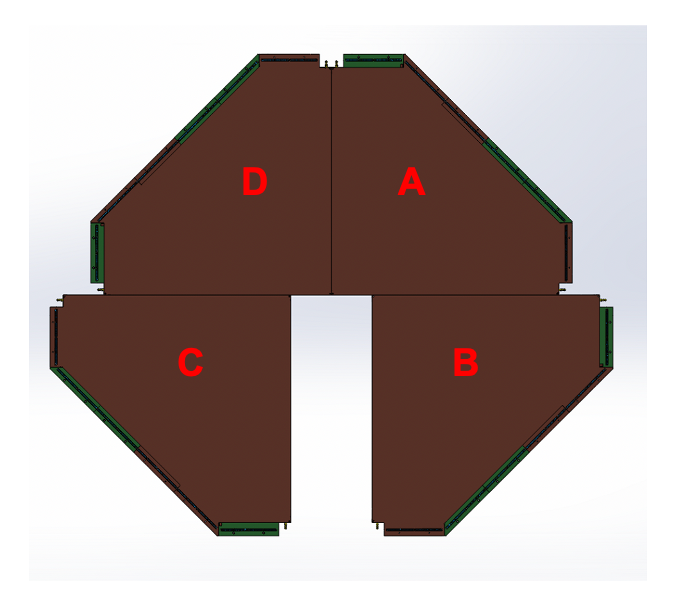
\includegraphics[width=0.7\textwidth,clip]{figures/Chapter2/sTGC.png}
    \end{center}
    \caption[前向小气隙室径迹探测器单个平面正视图]{前向小气隙室径迹探测器单个平面正视图,每个平面由四个五边形sTGC模块组成。}
    \label{fig:sTGC}
\end{figure}

笔者在攻读博士学位期间参与了sTGC在布鲁克海文国家实验室的测试以及cluster finder编写工作,将在接下来的几个小节中对窄隙室以及笔者的工作进行详细介绍。
\section{窄读出条窄隙室——sTGC}
\label{chap:3_2}

在粒子物理实验中,人们需要对产生的粒子的状态进行记录才能进行后续的物理分析,这样粒子探测器就应运而生。粒子探测器经过精巧的设计,当粒子通过探测器的过程中与探测器中的物质发生反应,人们通过收集反应产生的次级粒子如光子、电子等信息来反推通过探测器的粒子的信息。粒子探测器的种类有很多,以与粒子发生相互作用的介质分类的话,粒子探测器可以分成气体探测器,液体探测器,固体探测器等几个大类。气体探测器因为其造价相对便宜、可以大规模制作等优点得到了广泛的应用,许多大型粒子物理实验如BES、STAR、ALICE等都将其用作主要的径迹探测器。在这一章当中主要介绍的窄读出条窄隙室也是一种气体探测器。

在十九世纪七十年代之前,对于粒子径迹的探测手段主要是“照相”式的。以云室为例,当粒子通过充满了蒸汽的云室时和气体分子相互作用发生电离产生电子-离子对,这些电子-离子对作为凝结核使蒸汽凝成可见的雾珠。这样就使得不可见的粒子在穿过云室时留下可见的轨迹供人们进行分析。但这种“照相”式的探测手段的计数频率很低,极大地限制了实验的探测效率,人们希望能有电子学式的探测器,这样就可以极大地提高探测效率和径迹的信息收集能力。

在当时,正比计数器就已经被大量地应用在了射线的能谱测量当中,虽然可以通过将大量正比计数管组合在一起的方式来进行径迹探测,但是因为正比计数管本身的结构问题,这种解决方案的位置分辨有限且机械结构复杂。最开始人们曾经设想过是否可以在一个大的气体容器中平行地排列许多丝结构,但大多数人认为这样丝和丝之间会因为电容耦合效应导致信号传递到相邻的丝上,从而使得位置分辨变差。直到1968年,Charpak等人研究发现多丝结构可以按照预期设想工作并且获得很好的位置分辨,并据此发明了多丝正比室。恰帕克本人也因此获得了1992年的诺贝尔物理学奖。之后各种多丝室以及基于多丝室的探测器被不断地发明出来,成为了现在大型粒子物理实验的主力探测器。

窄读出条窄隙室(small-strip Thin Gap Chamber, sTGC)就是一种工作在饱和模式下的多丝室。sTGC的工作气体为55\%的二氧化碳和45\%的正戊烷组成的混合气体,阳极丝上加2900V的高压。
如图\ref{fig:sTGC}所示,STAR前向升级当中的窄隙室径迹探测器每一层由四个五边形的模组(Module)组成,四个不同的模组分别位于四个象限。以第一象限的A模组为第一块,之后每个象限的模组安置方式为A模组旋转(象限数-1)$*(-\frac{\pi}{2})$得到。每一个模组又由两个窄隙室组成。对于每一个窄隙室来说,两侧的阳极板背面均有读出条,其中一面读出条方向垂直于阳极丝,另一面读出条方向沿垂直于对角线方向,参见图\ref{fig:sTGC_chamber}。以第一象限的模组为例,从上到下的读出条方向分别为垂直于对角线方向,水平方向,竖直方向,垂直于对角线方向。从上往下各层的阳极丝和读出条方向如图\ref{fig:sTGC_chamber}中从左到右各图所示。

\begin{figure}[htb]
    \centering
    \begin{subfigure}[b]{0.3\textwidth}
        \centering
        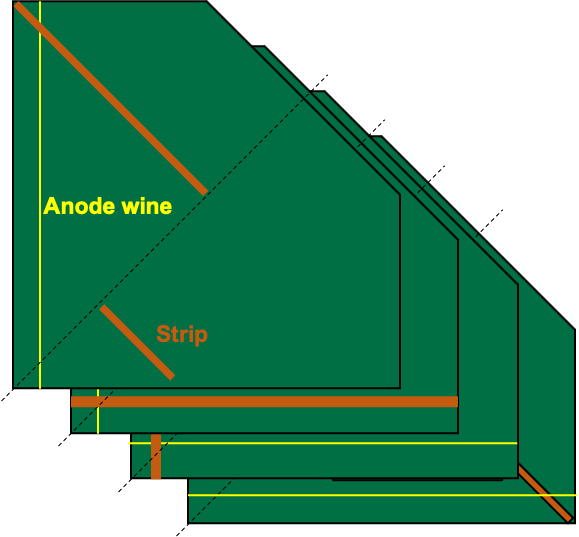
\includegraphics[width=\textwidth,clip]{figures/Chapter3/sTGC_Layers.png}
        \caption{}
        \label{fig:sTGC_Layers}
    \end{subfigure}
    \hfill
    \begin{subfigure}[b]{0.65\textwidth}
        \centering
        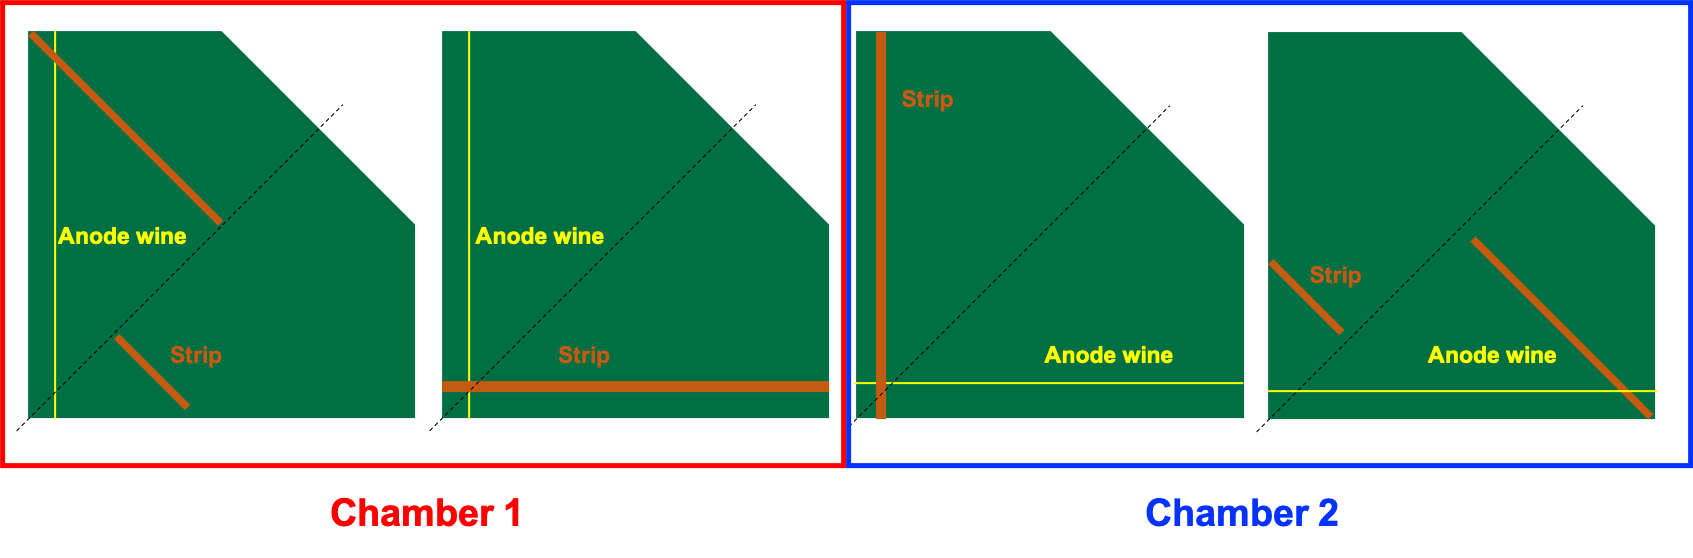
\includegraphics[width=\textwidth,clip]{figures/Chapter3/sTGC_chamber.png}
        \caption{}
        \label{fig:sTGC_chamber}
    \end{subfigure}
    \caption[sTGC 模组结构示意图]{\ref{fig:sTGC_Layers}为一个sTGC模组从上到下四层的阳极丝以及读出条的排列顺序。右边四个图为\ref{fig:sTGC_Layers}从上到下的展开,其中前两层和后两层分属不同的室}
       \label{fig:sTGC_All_Layers}
\end{figure}

sTGC的侧视图如图\ref{fig:sTGC_sideview}所示。上下两层为覆盖有石墨的FR4板,涂有石墨的两面相对,作为探测器的阴极,相隔2.8mm。阳极丝位于两个FR4板的中间,距离两板各1.4mm。在石墨涂层的背面是铜读出条(strip)。读出条宽2.7mm,读出条和读出条之间的间隙为0.5mm。读出条的长度根据读出条所在的位置不同有所不同,但大部分读出条的长度约为160mm左右,远大于读出条的宽度。当粒子在窄隙室的阳极丝附近发生电离的时候发生雪崩过程,在读出条上产生感应信号,电子学可以收集这个感应信号并且将其转化成为数字信号储存起来,以供后期数据分析。
\begin{figure}[htb]
    \begin{center}
    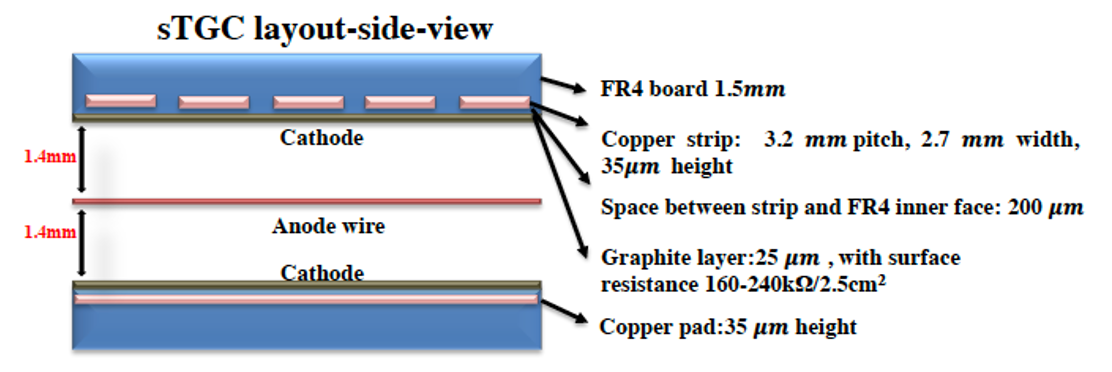
\includegraphics[width=0.7\textwidth,clip]{figures/Chapter3/sTGC_side_view.png}
    \end{center}
    \caption[sTGC内部结构示意图]{sTGC内部结构示意图}
    \label{fig:sTGC_sideview}
\end{figure}

当粒子通过阳极丝附近的时候,在工作气体中电离产生原初电子-离子对。电子开始向阳极丝附近漂移,而离子开始向阴极方向漂移。因为阳极丝上加有高压,电子在一个平均自由程内可以获得足够的能量使气体再次电离,从而在下次和气体分子碰撞的时候发生次级电离产生新的电子-离子对,次级电子-离子对又可以引发新的电离,从而使得电子-离子对的数目成指数形式增加。这个过程叫做雪崩过程。雪崩过程中电子会向阳极丝移动,产生感应信号后被阳极丝吸收。而离子因为质量较大,且所处位置远离阳极丝场强相对较小,所以移动速度相比于电子来说较慢。这些移动较慢的阳离子会在阳极丝附近形成“阳离子鞘”并向阴极移动。这个过程中在阴极背面的读出条上产生感应信号。整个雪崩过程的示意图参见图\ref{fig:Avalanche}。电子学和读出条相连接,将这个感应信号读出。在收集到每个读出条的感应电荷信号之后,我们就可以通过电荷重心法来计算粒子通过窄隙室时发生电离的位置。计算公式为:

\begin{equation}
    \label{eq:center_of_gravity}
    x = \frac{\Sigma X_i*Q_i}{\Sigma Q_i} 
\end{equation}
其中$x$为重建出的电离发生的位置,$X_i$为产生感应信号的读出条的位置,$Q_i$为在对应的读出条上面产生的感应信号的大小。

\begin{figure}[htb]
    \begin{center}
    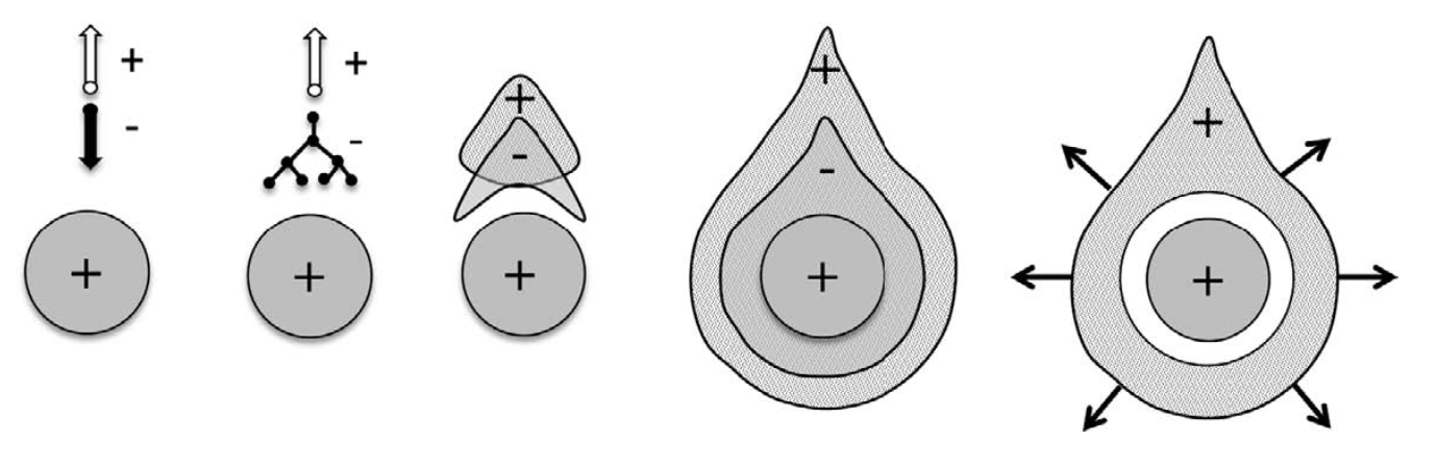
\includegraphics[width=0.7\textwidth,clip]{figures/Chapter3/Avalanche.png}
    \end{center}
    \caption[电子-离子对在阳极丝附近雪崩示意图]{电子-离子对在阳极丝附近雪崩示意图}
    \label{fig:Avalanche}
\end{figure}

从重建公式可以看出,对于沿着一个方向的读出条,我们只能重建出来和读出条垂直方向上的位置坐标。即沿着水平方向的读出条只能读出竖直方向上的位置坐标信息。这样四个读出层分别可以读出沿对角线方向、竖直方向、水平方向、沿对角线方向的一维位置坐标,如果需要得到二维的位置坐标我们需要对一维坐标进行配对,这就带来了ghost hit的问题。垂直于对角线方向的读出条和读出条本身的分组就是为了降低ghost hit的数目而设计的。关于这个问题将会在slow simulator和cluster finder一章进行详细讨论。
\section{sTGC于BNL测试部分}

在STAR-sTGC升级的前期研发过程中,山大一共制作了两个原型机用来进行测试,两个原型机尺寸分别为30cm$*$30cm和60cm$*$60cm,在后文中两个原型机将分别被称为小原型机和大原型机。每个原型机均由读出条方向相互垂直的两个独立的窄隙室组成。

小原型机于2019年1月寄到BNL,于2019年5月开始BNL的本地测试工作,并于2019年6月安装到STAR上进行束流测试。对于小原型机的测试工作主要分为两部分:一部分为在超净室(Clean Room)当中进行宇宙线测试,另一部分工作为束流测试。因为正戊烷易燃易爆的特性,在2019年初STAR并没有获得BNL使用正戊烷的安全许可,所以在前期的测试过程中工作气体主要为为TPC工作气体P10(90\%氩气和10\%甲烷的混合气体)和C10(90\%氩气和10\%二氧化碳的混合气体)。当2019年的run结束的时候小原型机再次回到超净室进行测试时才开始使用正戊烷作为工作气体进行测试。大原型机于2019年1月制作完成,在山大测试之后于2020年7月寄到BNL进行测试,于同年10月安装到STAR上进行测试。在大原型机的测试中同时对两种不同的读出电子学进行了测试。关于两个原型机的测试结果将在本小节进行详细的介绍。

于2021年,制作好的五边形模组逐渐从山大寄到BNL,为了保证所有模组可以正常工作,要对模组使用安装在STAR时所用的电源进行漏电流测试,测试的过程和结果也会在本小节中进行介绍。

\subsection{小原型机测试}

\subsubsection{超净室测试}

在STAR的超净室中,首先进行的是电子学测试。在2019年的时候,sTGC使用的是和STAR的时间投影室相同的前端电子学(TPX 电子学)。此电子学为波形取样型读出,可以将波形沿着时间分成每25ns一个的time bin,在每个time bin当中将在此time bin当中收集到的电荷信号转换成数字信号(ADC)读出。图\ref{fig:TPXChannel}为TPX电子学读出时一个通道的信号读出形式。
\begin{figure}[htb]
    \begin{center}
    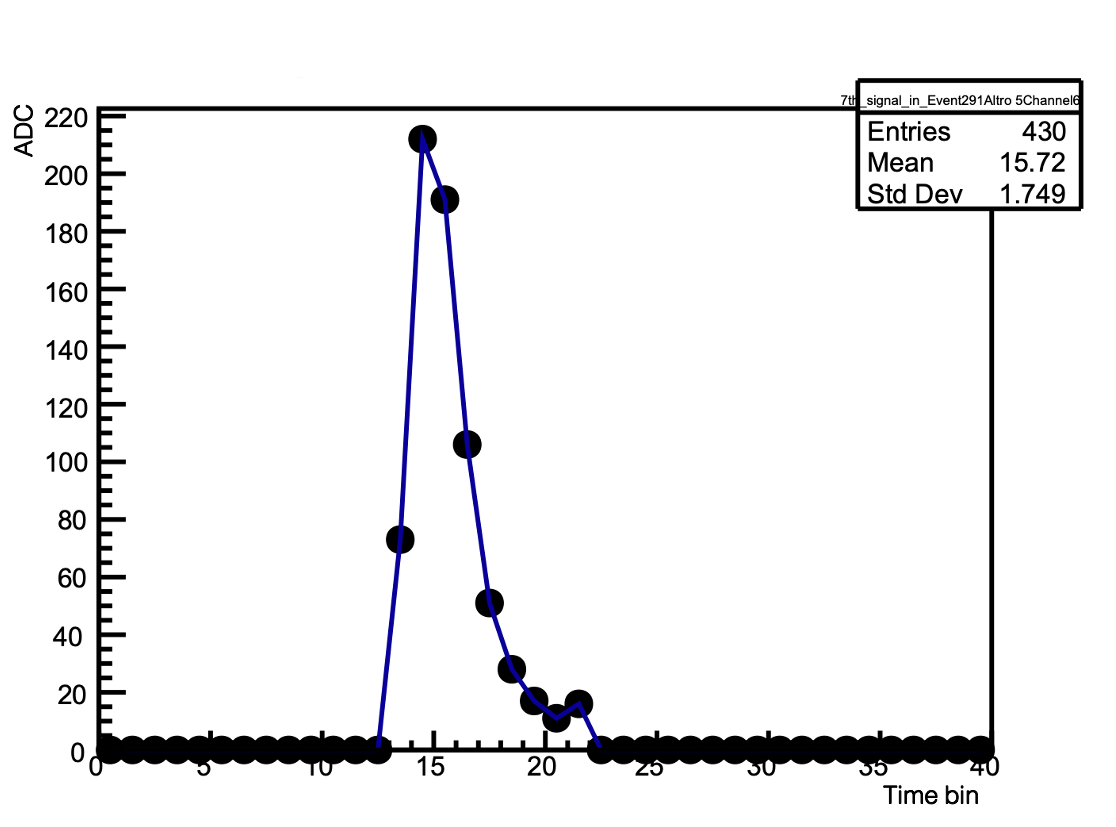
\includegraphics[width=0.7\textwidth,clip]{figures/Chapter3/TPXChannel.png}
    \end{center}
    \caption[TPX电子学单个channel信号读出分布]{TPX电子学单个channel信号读出分布,横轴为time bin,每个time bin时间长度为25ns。纵轴为对应time bin读出的ADC的值}
    \label{fig:TPXChannel}
\end{figure}
整个探测器的触发使用三块闪烁体作为触发系统。触发系统的设置如图\ref{fig:sTGC_Trigger_CR}所示。两个小闪烁体(8cm $*$ 16cm)紧贴探测器放置在小原型机的上下两侧,另一块较大的闪烁体(23cm $*$ 51cm)放置在探测器测试所用平台的下方,三个闪烁体末端接光电倍增管并且通过信号线将其连入信号甄别器,再联入符合单元。当宇宙线穿过闪烁体产生信号被光电倍增管收集到并传入信号甄别器以后,信号甄别器将其转换成负电压的方波信号。每个闪烁体的信号在经过信号甄别器后再被引入符合单元当中,当三个经过信号甄别器的信号被同时引入符合单元的时候符合单元输出一个信号进入trigger board当中,触发探测器电子学采集信号。在此设置之下宇宙线的触发频率大约为30 event/min。
\begin{figure}[htb]
    \begin{center}
    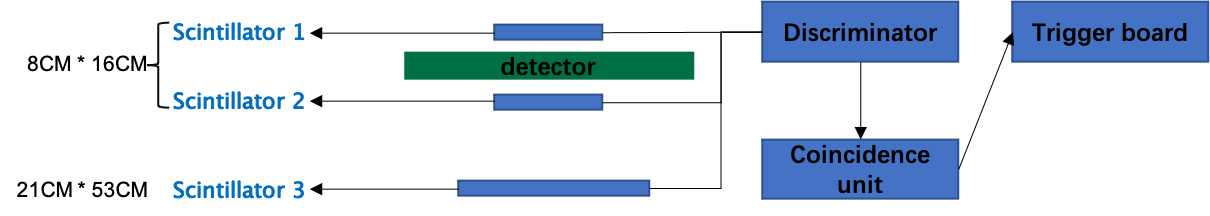
\includegraphics[width=0.7\textwidth,clip]{figures/Chapter3/TiggerCarton.png}
    \end{center}
    \caption[sTGC BNL超净室测试触发系统设置示意图]{sTGC BNL超净室测试触发系统设置示意图}
    \label{fig:sTGC_Trigger_CR}
\end{figure}

在2019年6月之前的测试当中,工作气体为C10,两个室高压均为1425V。在前期测试当中,首先利用丝端读出来验证是否探测器是否可以成功地采集信号。当可以通过丝端读出宇宙线的脉冲信号之后,整个探测器和电子学被接入到数据采集系统(Data Acquisition system, DAQ)当中进行取数。原始的.sfs文件经过解码后得到STAR标准的.daq文件,再通过STAR库中的bfc.C和StRoot中与sTGC相关的maker保存成为常用的ROOT文件格式。

在得到数据之后首先要完成的是数据中的通道和探测器当中实际的每个读出条的对应工作,即map的编写。在山大的小原型机测试中此工作已经完成,只需要将整理得到的文件写成头文件整合到z相关的maker当中去即可。对于19年测试使用的TPX电子学,每个前端电子学板(Front End Electronic Card, FEE Card)上共有两个ALTRO芯片,每个ALTRO芯片上共有16个通道(Channel),每个通道和一个读出条相连接。而不同的前端电子学板上的ALTRO芯片读出时的编号随着前端电子学板的编号变化而变化,这样我们就可以根据电子学读出时的ALTRO芯片编号和通道编号得到唯一对应的读出条编号。示意图见\ref{fig:TPX_map}。从而确定每个信号对应的空间位置来进行之后的效率分析。同时在大原型机和最后的前向窄隙室经济探测器中cluster的重建也需要map,因为后期sTGC的电子学更换为VMM电子学,所以map的对应方式也发生了一些改变。在之后会进行介绍。
\begin{figure}[htb]
    \begin{center}
    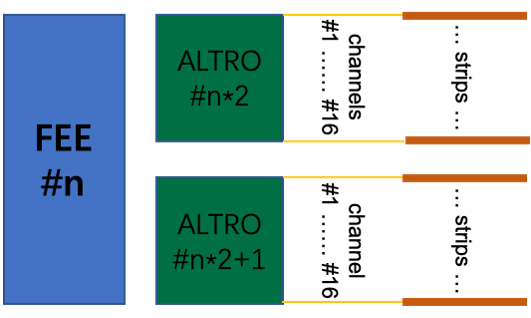
\includegraphics[width=0.7\textwidth,clip]{figures/Chapter3/TPX_map.png}
    \end{center}
    \caption[sTGC TPX电子学与读出条对应示意图]{sTGC TPX电子学与读出条对应示意图}
    \label{fig:TPX_map}
\end{figure}

当电子学正确设置并且可以读出信号之后,接下来的任务就是信号挑选和测试小原型机在C10气体下的效率表现。当工作气体为C10的时候,工作高压在1450V附近,当继续加高电压的时候会发生打火现象影响测试。

首先需要确定探测器的噪声水平,即当电子学接入探测器但探测器高压为0V时电子学可以读到的ADC分布。在此种情况下读到的ADC即为整个探测器和电子学在空负载情况下的噪声水平。因为需要接收宇宙线信号,整个小原型机水平放置,很自然地两个窄隙室被分别称为 top chamber 和 bottom chamber。两个窄隙室在0V下的噪音水平如图\ref{fig:ADC_Distribution_0V}所示。top chamber 和 bottom chamber的噪音水平分别为15ADC 和 20ADC。这两个噪音水平将会作为pedestal参与分析。但在2019年6月最开始的数据分析当中,为了对探测器效率有初步概念,pedestal取得相对较为宽松,两个室均为10ADC。
\begin{figure}[htb]
    \begin{center}
    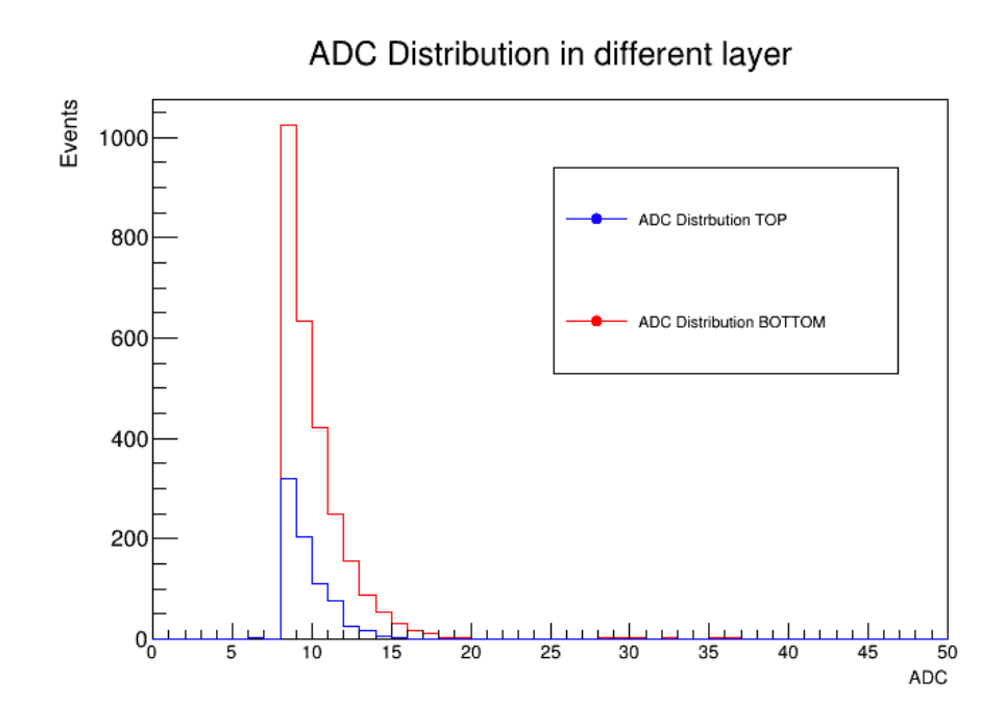
\includegraphics[width=0.7\textwidth,clip]{figures/Chapter3/ADC_Distribution_0V.png}
    \end{center}
    \caption[0V和C10气体下小原型机ADC分布]{0V和C10气体下小原型机ADC分布,蓝色直方图为top chamber的ADC分布,红色直方图为bottom chamber的ADC分布}
    \label{fig:ADC_Distribution_0V}
\end{figure}

当map正确工作后对于每一个事例我们就可以得到这样的一个三维分布:x轴和y轴分别为读出条编号和time bin,z轴为每个读出条在该time bin当中的ADC对应的值。一个事例当中的三维分布如图\ref{fig:Signal_3D}所示。可以看到当加上高压的时候和不加高压相比,信号持续时间和信号的宽度明显的变宽,在初步的分析当中对于信号的宽度和持续时间我们设置了如下的信号判选条件:
\begin{itemize}
    \item 对于单个读出条要求连续的ADC > pedestal的time bin个数大于3。此时认为该读出条有信号响应。
    \item 对于有信号响应的读出条,当相邻的有信号响应的读出条的个数大于3根的时候认为有一个宇宙线事例。
\end{itemize}
\begin{figure}[htb]
    \centering
    \begin{subfigure}[b]{0.45\textwidth}
        \centering
        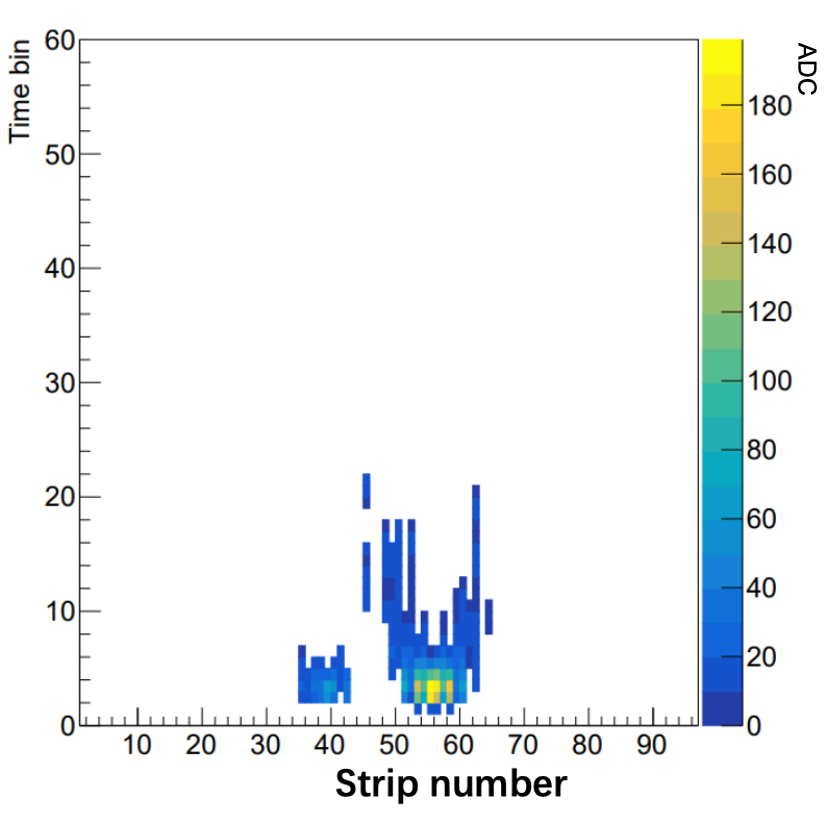
\includegraphics[width=\textwidth,clip]{figures/Chapter3/Strip_TB_ADC.png}
        \caption{1450V}
        \label{fig:Strip_TB_ADC}
    \end{subfigure}
    \hfill
    \begin{subfigure}[b]{0.45\textwidth}
        \centering
        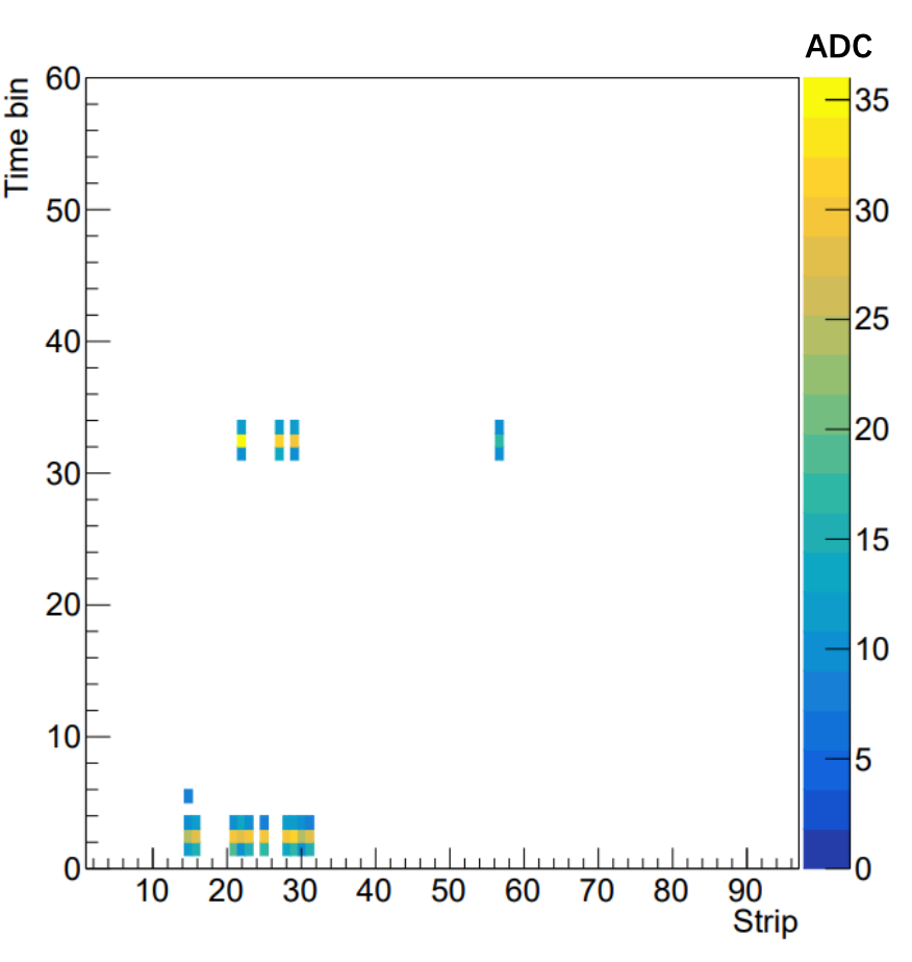
\includegraphics[width=\textwidth,clip]{figures/Chapter3/Strip_TB_ADC_noise.png}
        \caption{0V}
        \label{fig:Strip_TB_ADC_noise}
    \end{subfigure}
    \caption[一个事例当中每个读出条上ADC随time bin 分布示意图]{\ref{fig:Strip_TB_ADC}为bottom chamber在高压为1450V下一个信号事例。\ref{fig:Strip_TB_ADC_noise}为bottom chamber在高压为0V下的一个噪音事例。}
       \label{fig:Signal_3D}
\end{figure}
其中根据测试环境的变化pedestal的值可能发生变化,在首次测试当中pedestal取10,top chamber和bottom chamber的高压分别为1450V和1350V。在此设置下,根据这样的宇宙线事例挑选条件我们对在超净室取得的第一个run进行了分析,结果如图\ref{fig:Cosmic_first}所示。对于效率的计算分别采取了以下两种计算方式:
\begin{itemize}
    \item 宇宙线触发。
    \\效率计算公式如下:$\epsilon_{top(bottom)~chamber} = N_{top(bottom)~chamber}/N_{cosmic~event}$
    \item 窄隙室相互触发。
    \\效率计算公式如下:$\epsilon_{top(bottom)~chamber} = N_{two~chambers}/N_{bottom(top)~chamber}$
\end{itemize}
其中$N_{cosmic~event}$为总的宇宙线触发事例数,$N_{top(bottom)~chamber}$为一个事例当中top(bottom) chamber有信号响应的事例数,$N_{two~chambers}$为一个事例当中top和bottom chmaber同时有信号响应的事例数。在这个run当中的各种计算方式下的效率如表\ref{tab:Cosmic_first}所示:
\begin{table}[h!]
    \centering
    \caption{小原型机BNL本地测试第一个宇宙线run效率测试结果}
    \label{tab:Cosmic_first}
    \begin{tabularx}{0.9\textwidth} {| >{\centering\arraybackslash}X |>{\centering\arraybackslash}X |>{\centering\arraybackslash}X |>{\centering\arraybackslash}X |}
        \hline
         &高压& 宇宙线触发 & 窄隙室相互触发\\
        \hline
        top chamber & 1450V & 2.5\% & 17.5\%\\
        \hline
        bottom chamber& 1350V & 0.4\% & 2.7\% \\
        \hline
    \end{tabularx}
\end{table}
\begin{figure}[htb]
    \begin{center}
    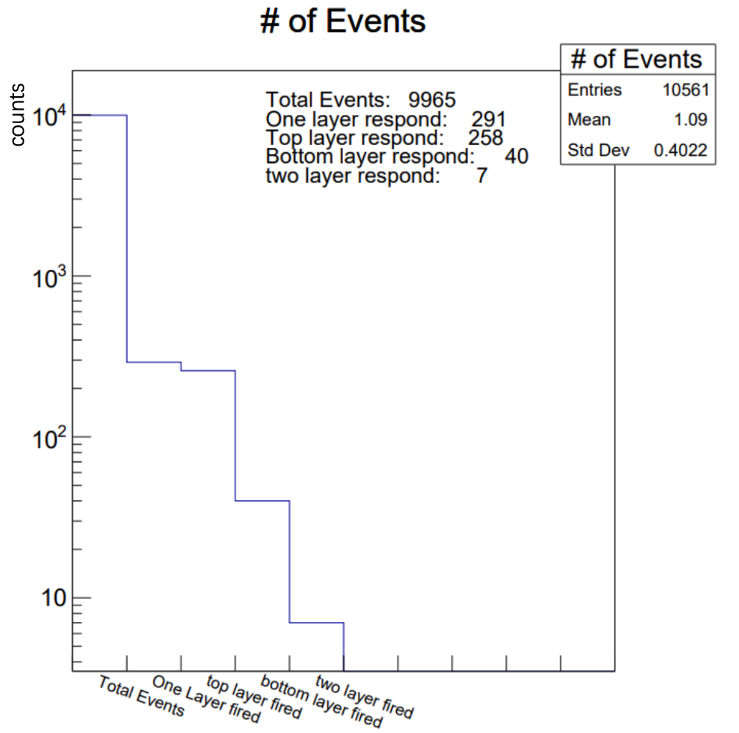
\includegraphics[width=0.7\textwidth,clip]{figures/Chapter3/Cosmic_first.png}
    \end{center}
    \caption[小原型机第一个宇宙线run的测试结果]{小原型机第一个宇宙线run的测试结果,其中total events 为总的触发事例数,one layer fired 为在一个事例当中top 或者 bottom chamber有信号的事例数,top layer fired和bottom layer fired分别为一个事例中top和bottom chamber有信号的事例数,two layers fired为一个事例中两个chamber同时能找到信号的事例数。}
    \label{fig:Cosmic_first}
\end{figure}
可以看到初步测试的结果显示在使用C10气体作为工作气体的情况下整个探测器的探测效率很低,无法满足正常的使用需求。在2019年9月,STAR获得了在超净室当中使用正戊烷的许可,对C10和正戊烷两种工作气体下的探测器表现进行了进一步的研究。

首先测试的是在相同高压下对两种不同的工作气体的流速对探测效率的影响。在不同工作气体工况下保持高压不变,在气体流速为80 cc/min 和 200 cc/min下进行测试。C10气体下两个chamber的高压均设置为1425V,正戊烷为工作气体时两个chamber高压均为2800V。信号挑选的判选条件如表\ref{tab:Cosmic_gasflow}所示
\begin{table}[h!]
    \centering
    \caption{气体流速测试宇宙线信号挑选判选条件}
    \label{tab:Cosmic_gasflow}
    \begin{tabularx}{0.9\textwidth} {| >{\centering\arraybackslash}X |>{\centering\arraybackslash}X |>{\centering\arraybackslash}X |>{\centering\arraybackslash}X |>{\centering\arraybackslash}X |}
        \hline
         & timming &ADC pedestal& 单信号条信号持续时间 & 信号宽度\\
        \hline
        C10 & 0-30 time bin & 10 ADC & >3 time bin & > 3 strips\\
        \hline
        ${\rm CO_2}$ + n-Pentane& 0-30 time bin & 10 ADC & >3 time bin & > 3 strips\\
        \hline
    \end{tabularx}
\end{table}
在不同流速下的效率测试结果显示不论是C10还是正戊烷作为工作气体,探测器的效率都没有发生明显的改变,结果如图\ref{fig:GasFlow}所示。证明探测器可以在不同的气体流速下稳定工作。同时可以看到,当正戊烷作为工作气体的时候探测器可以达到很高的探测效率,99约\%,符合探测器设计时的高效率的要求。
\begin{figure}[htb]
    \begin{center}
    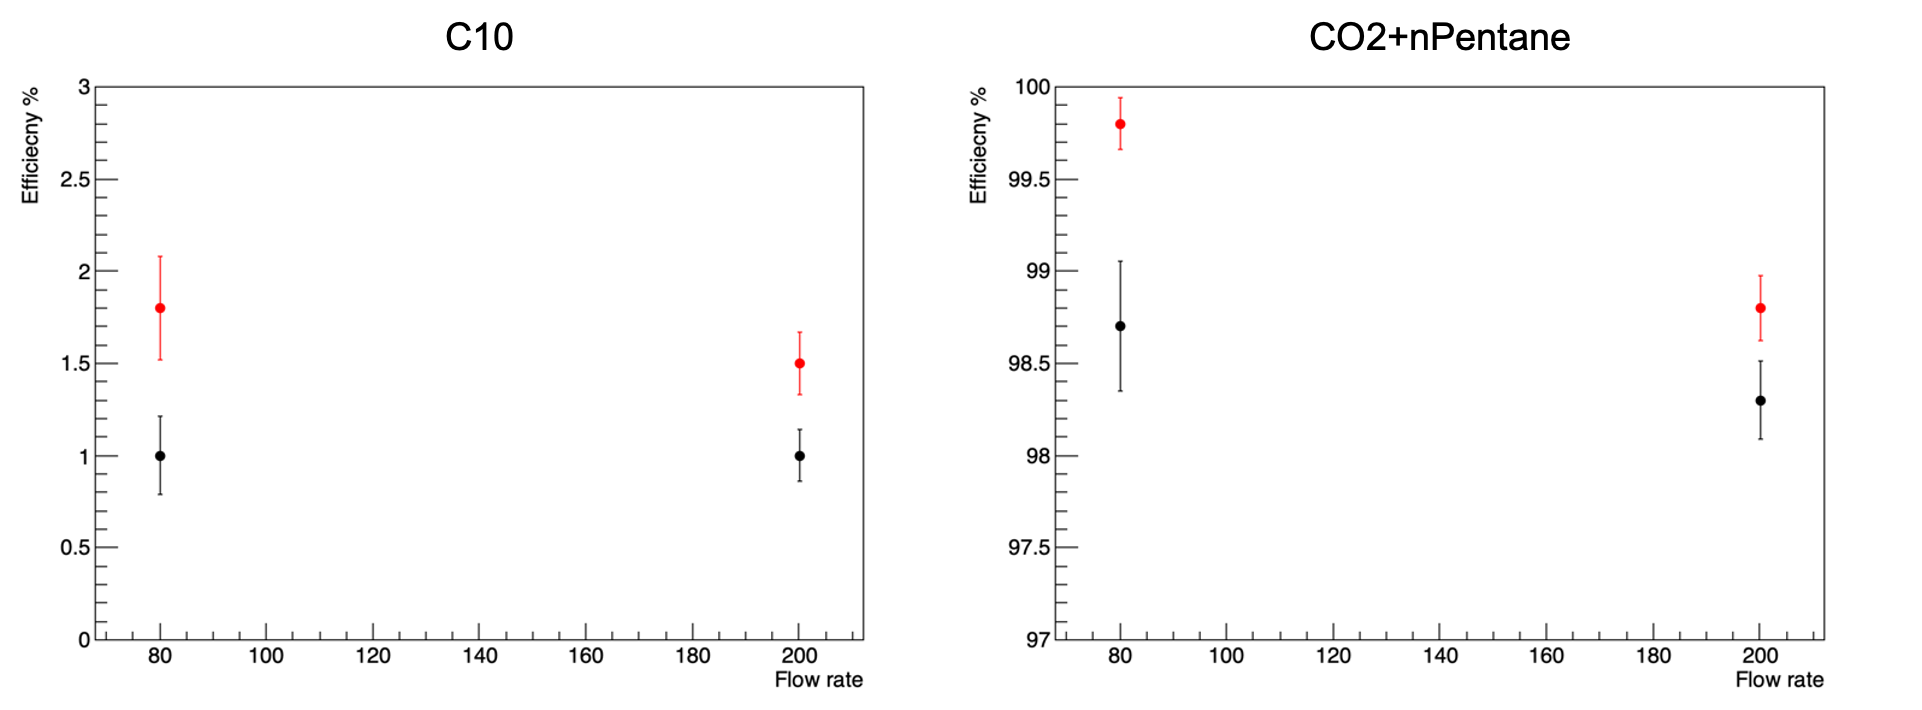
\includegraphics[width=0.9\textwidth,clip]{figures/Chapter3/GasFlow.png}
    \end{center}
    \caption[小原型机不同气体不同流速效率测试结果]{小原型机不同气体不同流速效率测试结果。左图工作气体为C10气体,右图工作气体为${\rm CO_2}$ + n-Pentane}
    \label{fig:GasFlow}
\end{figure}

根据参考文献[],在相同的气压下正戊烷的在混合气体当中所占的百分比和温度正相关,因为气体混合系统并不是完美的混合系统,气体的温度或者组分会在一定范围内浮动,所以我们也需要测试当正戊烷在不同的温度情况下的探测效率表现。测试时气体流速固定均为80 cc/min,信号判选条件以及高压和流速测试时判选条件相同。测试结果如图\ref{fig:Temperature}所示。可以看到当温度在${\rm 15^{\circ}C}$ 至 ${\rm 19^{\circ}C}$的范围内浮动时整个探测器都可以保持很高的探测效率,工作状况稳定,在目标的温度范围内探测器可以稳定工作。
\begin{figure}[htb]
    \begin{center}
    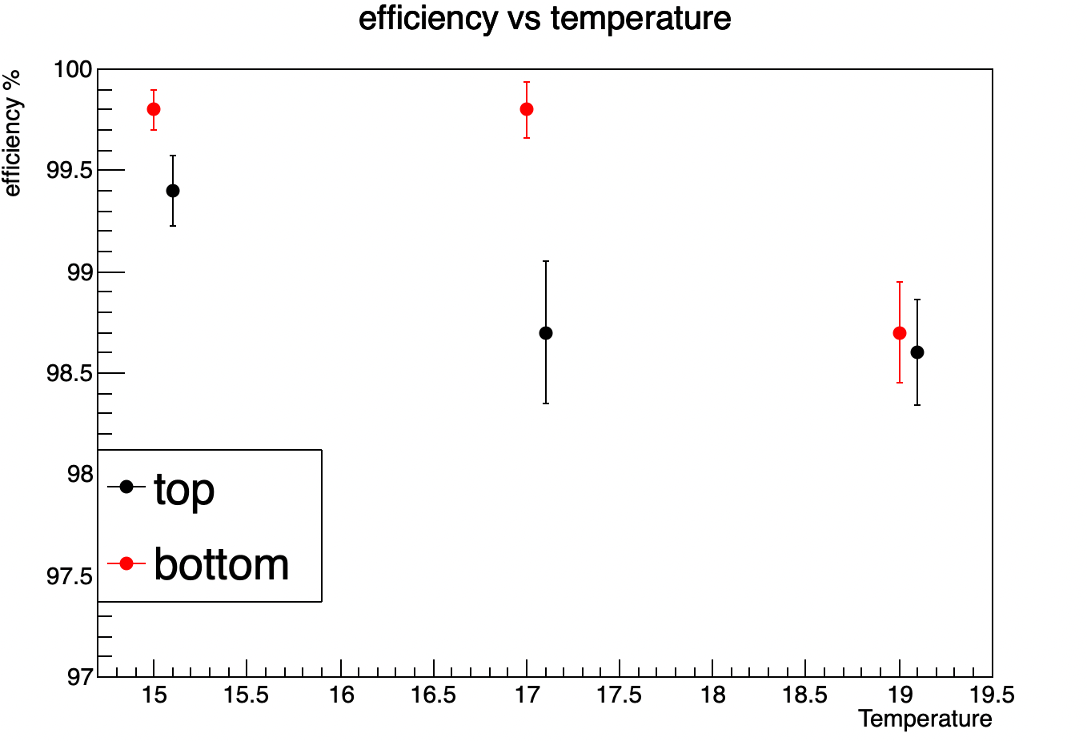
\includegraphics[width=0.75\textwidth,clip]{figures/Chapter3/Temperature.png}
    \end{center}
    \caption[小原型机正戊烷工作气体下不同温度效率测试结果]{小原型机正戊烷工作提起不同温度效率测试结果,黑色圆点为top chamber结果,红色圆点为bottom chamber结果}
    \label{fig:Temperature}
\end{figure}

除了对C10和正戊烷作为工作气体进行测试以外,我们还尝试了对其他几种工作气体进行测试,试图找出可以替代正戊烷的工作气体以避免因为正戊烷的可燃性而带来的工程以及安全问题。但经过了几组不同的工作气体测试后发现除了正戊烷以外其余的工作气体均无法达到预期的探测效率,结果如表\ref{tab:CR_DifferentGas}所示。
\begin{table}[h!]
    \centering
    \caption{不同工作气体小原型机效率测试结果}
    \label{tab:CR_DifferentGas}
    \begin{tabularx}{0.95\textwidth} {| >{\centering\arraybackslash}X |>{\centering\arraybackslash}X |>{\centering\arraybackslash}X |>{\centering\arraybackslash}X |}
        \hline
         & 工作气体 & 高压 & 效率 \\
        \hline
        top chamber & Ar+${\rm CO_2}$+${\rm CH_4}$ & 2200 V & 6.2\%  \\
        \hline
        bottom chamber& Ar+${\rm CO_2}$+${\rm CH_4}$ & 2200 V& 2.5\% \\
        \hline
        top chamber & Ar+${\rm CO_2}$+${\rm CH_4}$ & 2300 V & 10.3\%  \\
        \hline
        bottom chamber& Ar+${\rm CO_2}$+${\rm CH_4}$ & 2300 V& 3.3\% \\
        \hline
        top chamber & Ar+${\rm CO_2}$+异丁烷 & 2200 V & 5.8\%  \\
        \hline
        bottom chamber& Ar+${\rm CO_2}$+异丁烷& 2200 V& 2.3\% \\
        \hline
    \end{tabularx}
\end{table}

\subsubsection{束流测试}

在第一次超净室测试验证了TPX电子学可以正常的在小原型机上工作并且取数以后,于2019年6月小原型机被安装在了STAR的西侧进行取数测试其在束流环境下的表现。触发使用STAR minimum bias(MiniBias, MB) trigger。但在2019年的run当中,MB trigger 并不是专门为前向的探测设计的trigger,无法通过trigger的数目来作为效率测试的分母。所以对于效率的测试只能使用互相触发的方式来进行。

在小原型机的束流测试中,我们对探测器进行了高压扫描。同样因为安全许可问题,在2019年的束流测试中只能使用C10作为工作气体。首先在高压为0 V时进行取数来确定pedestal,单信号条信号持续时间,信号宽度等判选条件的取值。束流测试当中的信号判选条件设置如表\ref{tab:Beam_HVScan}所示:
\begin{table}[h!]
    \centering
    \caption{束流测试中高压扫描信号判选条件}
    \label{tab:Beam_HVScan}
    \begin{tabularx}{0.95\textwidth} {| >{\centering\arraybackslash}X |>{\centering\arraybackslash}X |>{\centering\arraybackslash}X |>{\centering\arraybackslash}X |>{\centering\arraybackslash}X |}
        \hline
         & timming &ADC pedestal& 单信号条信号持续时间 & 信号宽度\\
        \hline
        top chamber & < 10 time bin & 10 ADC & >3 time bin & > 3 strips\\
        \hline
        bottom chamber& < 10 time bin & 10 ADC & >3 time bin & > 3 strips\\
        \hline
    \end{tabularx}
\end{table}
高压扫描从1400 V开始,每隔25 V取数。当电压升到1500 V的时候探测器频繁出现打火问题,所以电压扫描到此为止。除了高压以外剩下的所有触发以及气体的设置均不变。探测器互相触发所测量到的效率如图\ref{fig:BeamHV}所示。在C10工作气体下探测器的工作效率随着高压的增加呈线性增加,但是仍然无法达到探测器设计时的效率要求。且因为最后的设计是多层sTGC作为整个径迹探测系统,如果单层只有25\%左右的探测效率,最后四层合并对于单条径迹的探测效率期望只有0.3\%,完全无法接受。所以C10作为工作气体的想法经过束流测试之后被完全否决。综合之前的不同气体组分的测试结果,正戊烷被最后确定为前向小读出条窄隙室径迹探测器的工作气体。
\begin{figure}[htb]
    \begin{center}
    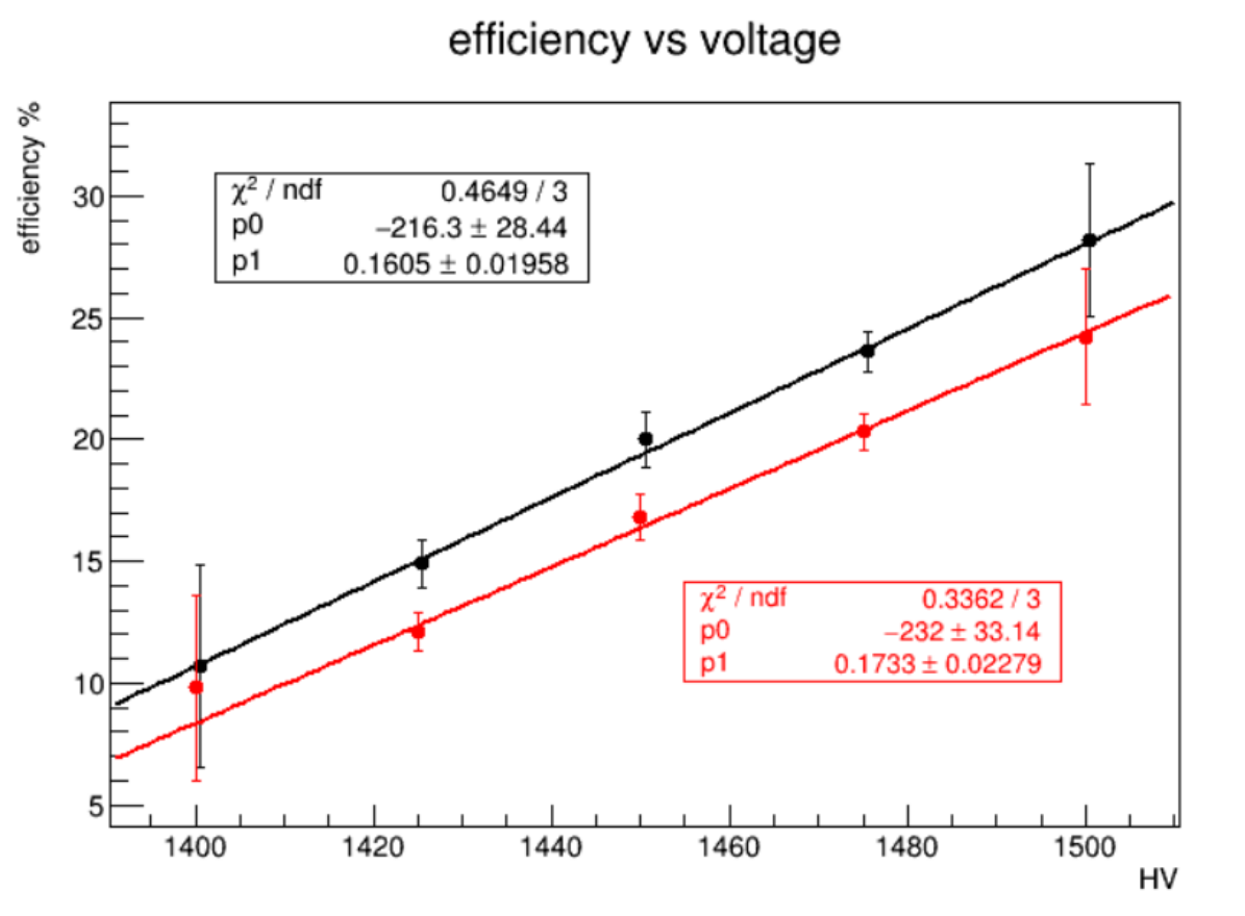
\includegraphics[width=0.75\textwidth,clip]{figures/Chapter3/BeamHVpng.png}
    \end{center}
    \caption[小原型机C10工作气体下束流环境中不同高压效率测试结果]{小原型机C10工作气体下束流环境中不同高压效率测试结果,黑色圆点为top chamber结果,红色圆点为bottom chamber结果。error bar 仅显示统计误差,和数据量直接相关,在1400V时因为探测效率很低、在1500V因为经常发生打火探测器停止工作所以数据量明显小于其他能量。}
    \label{fig:BeamHV}
\end{figure}
\subsection{大原型机测试}

对于大原型机的测试主要分为两个部分,一部分是气体系统以及Slow control系统的测试,另一部分为电子学测试以及数据分析。气体系统和Slow Control的工作主要由BNL的人员完成,在此不多做介绍。笔者主要参与的为电子学测试和数据分析工作。将接下来的部分中当中进行详细介绍。

和小原型机测试一样,首先需要解决的是电子学通道和实际读出条对应的map问题。因为在最终的探测器丝室的设计中读出条在同一个方向上分了好多段,所以大原型机也进行了类似的设计,在同一个方向上读出条被分成多段,这使得map工作相对于小原型机变得复杂了一些。大原型机的读出条和插口对应如图\ref{fig:LargePrototype_PCB}所示。在实际的原型机测试当中为了测试读出条分段对ghost hit的排除能力,要让左图右下角即读出条分段最多的部分相互重叠,这就要求一个室的布局应该是另一个室沿着左上到右下的对角线镜像反转。左图和右图分别为两个室的布局,其中右图为左图沿对角线反转后得到,和实际的原型机读出条分布相符。
这样就导致的读出条的编号方式需要进行改变,在小原型机当中读出条只有一列读出条,只需按照顺序编号即可,当有多行strip之后单纯按顺序编号会导致读出条编号混乱,无法直接使用小原型机的map文件,所以map需要重新编写。对于单个前端电子学板的通道和读出条对应的部分还是和图\ref{fig:TPX_map}所示相同,但读出条的编号发生了改变,编号从单纯的$n_{strip}$变成了($n_{row} * 1000 + n_{strip}$)。整个编号的最高位为行号。插口号和读出条行号的对应关系见表\ref{tab:LargePrototype_map}。对于另一个室来说,因为发生了镜像翻转,FEE上的通道和读出条对应的关系也发生了翻转,需要在map的头文件里额外的添加函数来进行翻转。
\begin{table}[h!]
    \centering
    \caption{大原型机插口号和读出条行号对应关系}
    \label{tab:LargePrototype_map}
    \begin{tabularx}{1\textwidth} {| >{\centering\arraybackslash}X |>{\centering\arraybackslash}X |>{\centering\arraybackslash}X |>{\centering\arraybackslash}X |}
        \hline
        行号 & 1 & 2 & 3 \\
        \hline
        插口号& 1 4 7 & 2 5 8 10 12 14 & 3 6 9 11 13 15 \\
        \hline
    \end{tabularx}
\end{table}

\begin{figure}[htb]
    \begin{center}
    \includegraphics[width=0.8\textwidth,clip]{figures/Chapter3/LargePrototype_PCB.png}
    \end{center}
    \caption[sTGC 大原型机Strip示意图]{sTGC 大原型机Strip示意图白色数字标明了不同的插口对应的strip区域,例如当前端电子学卡插在编号为1的slot上时将会和编号为1的读出条区域相连接。左图和右图分别为大原型机两个不同室的读出条分布。}
    \label{fig:LargePrototype_PCB}
\end{figure}

同时因为大原型机的前端电子学插口是为了TPX电子学所设计的,而最终sTGC使用的电子学是VMM芯片,并不能直接连接到大原型机的电子学插口上面去,需要一个转接器来让VMM电子学可以插到TPX电子学对应的插口上面去。这就使得当使用VMM电子学进行测试的时候,map的头文件里需要额外添加一个关于VMM电子学通道和TPX电子学通道对应的函数。


\subsection{五边形模组漏电流测试}

从2021年初开始,在山大制作完成的五边形模组被陆续寄到BNL,等待测试和组装。因为这一批模组是最后组装成为前向窄隙室径迹探测器的模组,所以说需要进行长时间的高压打火测试,来保证探测器可以长时间稳定地运行。所有的探测器在山大制作完成之后均进行过长时间的打火测试,结果被记录在了每个探测器的travller当中。图\ref{fig:S18_traveller}为S18在山大进行漏电流测试时的结果。可以看到在山大测试时漏电流很稳定且低于50nA。当探测器运到BNL后,如果一个模组没有因为在运输途中遇到意外而损坏的话,在通气24小时进行干燥之后就开始进行漏电流测试。
\begin{figure}[htb]
    \begin{center}
    \includegraphics[width=0.8\textwidth,clip]{figures/Chapter3/S18_traveller.png}
    \end{center}
    \caption[五边形模组S18山大漏电流测试结果]{五边形模组S18山大漏电流测试结果}
    \label{fig:S18_traveller}
\end{figure}

第一批被安全寄到BNL的模组为S18和S21,首先使用了LeCory作为电源对其进行了漏电流测试,在Jarda的帮助下通过Python脚本实现了对电流数据的记录。但因为LeCory电源本身读出系统的限制,数据记录系统的记录频率仅为4.6Hz。且无法设置trip time,只能使用LeCory自己内部的设置。同时在测试环境上,相比于山大位于超净室当中测试,可以控制整个环境的湿度和温度。BNL的超净室因为被占用,所以只能在Wide Angle Hall当中进行测试,无法控制环境的温度和湿度。测试时间处于夏季,湿度为大约55\%,对整个探测器的漏电流表现还是有一定的影响。从图\ref{fig:LeakCurrent_LeCory}中可以观察到,在加上高压之后漏电流需要一段时间以后才能稳定在较低的数值。

为了保证电源和探测器的安全,整个测试过程当中电压从1000V开始当漏电流稳定以后再升高500V,当漏电流再次稳定之后再升高电压。直到升高到2900V为止。以S18-C55为例,在1000-2500V下的漏电流表现如图\ref{fig:LeakCurrent_LeCory}所示,可以看到在加高压足够的时间之后,整个探测器的漏电流都会趋于稳定,但是普遍高于山大的漏电流测试结果。当使用LeCory尝试升高电压至2900V的时候,同时进行测试的S18和S21的四个室均发生了trip。之后决定在2800V进行更长时间的Burning之后在升到2900V进行测试。但是在这个过程中发生了LeCory电源的死机,死机重启后电源的表现变得比较奇怪。决定更换电源后重新进行测试。
\begin{figure}[htb]
    \begin{center}
    \includegraphics[width=0.8\textwidth,clip]{figures/Chapter3/LeakCurrent_LeCory.png}
    \end{center}
    \caption[五边形模组S18 BNL使用LeCory电源漏电流测试结果]{五边形模组S18 BNL使用LeCory电源漏电流测试结果}
    \label{fig:LeakCurrent_LeCory}
\end{figure}

之后的测试当中电源被更换为CANE SY5527,即当前向窄隙室探测器安装到STAR上之后会使用的电源。但同样因为读出系统的问题,电流数据记录的频率仅为约1.4Hz。但相比于LeCory电源,SY5527可以设置trip time。使用SY5527时的测试设置如表\ref{tab:SY5527Settting}所示。更换成SY5527之后测试方法和用LeCory测试时一样,从500V开始电压逐步升高,当漏电流稳定之后再将电压升到更高的电压。以S16-C22为例,在500、1000、1500、2500V时的电压表现分别如图\ref{fig:LeakCurrent_SY5527}所示。相比于LeCory,在低电压时SY5527的漏电流整体要高于LeCory的漏电流,约为200-300nA,但更加的稳定。在低电压下漏电流表现很稳定之后开始将电压升到2900V进行测试。
\begin{table}[h!]
    \centering
    \caption{SY5527漏电流测试设置}
    \label{tab:SY5527Settting}
    \begin{tabularx}{1\textwidth} {| >{\centering\arraybackslash}X |>{\centering\arraybackslash}X |>{\centering\arraybackslash}X |>{\centering\arraybackslash}X |}
        \hline
        trip current & trip time & ramp up speed & ramp down speed \\
        \hline
        2 ${\rm \mu A}$& 0.1s & 10 V/s & 20 V/s \\
        \hline
    \end{tabularx}
\end{table}
\begin{figure}[htb]
    \begin{center}
    \includegraphics[width=0.8\textwidth,clip]{figures/Chapter3/SY5227LeakCurret.png}
    \end{center}
    \caption[五边形模组S16 BNL使用CANE SY5527电源漏电流测试结果]{五边形模组S16 BNL使用CANE SY5527电源漏电流测试结果}
    \label{fig:LeakCurrent_SY5527}
\end{figure}

当电压升到2900V,漏电流的表现依旧相对稳定,约为500nA。但是观察到了比较奇怪且尖锐的峰,如图\ref{fig:LeakCurrent_SY5527_2900}所示。在8月1日的晚上出现了一个很尖锐的峰,在检查数据的时候发现峰值可以达到10${\rm \mu A}$级别,持续时间也大于所设置的tirp时间0.1s。且并不是一个漏电流逐渐上升的过程,漏电流会突然跳到很大的数值并在大约2-3s后再次回到之前的值。在之后的测试中也多次发现了这样奇怪的峰,但没有发生trip现象,探测器仍然稳定工作。最后经过排查怀疑是电源自带的电流读出系统的问题。在所有的五边形模组通过了漏电流测试以后前向窄隙室径迹探测器的组装工作随后开始。
\begin{figure}[htb]
    \begin{center}
    \includegraphics[width=0.8\textwidth,clip]{figures/Chapter3/LeakCurrent_SY5527_2900.png}
    \end{center}
    \caption[五边形模组S16 BNL使用CANE SY5527电源电压为2900V漏电流测试结果]{五边形模组S16 BNL使用CANE SY5527电源电压为2900V漏电流测试结果}
    \label{fig:LeakCurrent_SY5527_2900}
\end{figure}
\section{sTGC slow simulator 及 Cluster finder}

除了硬件测试的部分,对前向窄隙室探测器来说,另外一个很重要的部分是软件方面的工作。笔者主要参与了slow simulator的改进和cluster finder的编写工作。在本小节当中将要对此进行介绍。

slow simulator是一个基于ROOT且不依赖于STAR软件环境的小的模拟软件,主要用于当模拟探测器有击中的时候探测器响应的情况并且用起来进行cluster finder的初步测试工作。而cluster finder即为最后用于重建sTGC的击中的软件部分。

\subsection{slow simulator}

笔者参与工作的最新版本的slow simulator可以在笔者的Github上找到。整个slow simulator的工作流程如图\ref{fig:Simulator_flow}所示。
\begin{figure}[htb]
    \begin{center}
    \includegraphics[width=0.7\textwidth,clip]{figures/Chapter3/Simulator_flow.png}
    \end{center}
    \caption[sTGC slow simulator 工作流程示意图]{sTGC slow simulator 工作流程示意图}
    \label{fig:Simulator_flow}
\end{figure}

首先是对整个前向窄隙室径迹探测器的几何结构的定义。最终五边形构型的窄隙室模组的读出条分布如图\ref{fig:sTGC_PCB}所示,其中左图为沿着水平或者竖直方向读出条的分布,右图为沿着对角线方向的读出条的分布。可以看到整个读出条在水平和竖直方向上被分成了三组,在沿对角线方向上被分成了两组。因为这些读出条是通过不同的通道读出,所以在模拟的时候这些不同的组内的信号响应要分别进行模拟。在初版的simulator当中,对cluster响应信号的模拟是因为在探测器当中可以产生一个二维的高斯分布并往X与Y两个方向进行投影,其中高斯分布使用史迎迎在山大测试当中得到的信号宽度分布作为输入。但在后来的讨论当中发现,实际测试得到的高斯分布并不是一个二维的信号分布在一维上的投影,而是在一维方向上直接得到的。所以二维的高斯分布在模拟实际的信号响应的时候会有偏差,在之后的版本中对信号的模拟从二维的高斯分布调整成为了沿着垂直于读出条方向上的一维高斯分布,如图\ref{fig:Simulator_Cluster}右图所示。

\begin{figure}[htb]
    \centering
    \begin{subfigure}[b]{0.45\textwidth}
        \centering
        \includegraphics[width=\textwidth,clip]{figures/Chapter3/sTGC_PCB_HV.png}
        \caption{}
        \label{fig:sTGC_PCB_HV}
    \end{subfigure}
    \hfill
    \begin{subfigure}[b]{0.45\textwidth}
        \centering
        \includegraphics[width=\textwidth,clip]{figures/Chapter3/sTGC_PCB_Diag.png}
        \caption{}
        \label{fig:sTGC_PCB_Diag}
    \end{subfigure}
    \caption[五边形构型sTGC模组读出条分布示意图]{\ref{fig:sTGC_PCB_HV}读出条为水平或者竖直方向上的分布示意图。\ref{fig:sTGC_PCB_Diag}为沿对角线方向的读出条的分布示意图。}
       \label{fig:sTGC_PCB}
\end{figure}
\begin{figure}[htb]
    \begin{center}
    \includegraphics[width=0.85\textwidth,clip]{figures/Chapter3/Simulator_Cluster.png}
    \end{center}
    \caption[slow simulator 对cluster响应的模拟]{slow simulator 对cluster响应的模拟。左图为初版simulator对cluster响应的模拟,此时认为cluster在探测器当中产生的分布为二维的高斯分布,在没有cluster位置的bin当中的content为对噪音的模拟。右图为最新的simulator当中对cluster信号的模拟,已经改为两个方向上的高斯分布。右图当中没有对噪音的模拟。}
    \label{fig:Simulator_Cluster}
\end{figure}

在模拟的时候如何模拟打在边界的cluster是一个需要注意的问题。从图\ref{fig:sTGC_PCB}中可以看到,因为五边形构型的原因,读出条的分布并不是三组完全平行且每组当中所有读出条长度相同的三组读出条,而是在同一个方向有交界的三组。这样当一个粒子击中在读出条的边界的时候实际上会在两组读出条中同时产生信号。在模拟的时候需要注意当一个cluster在读出条组的边界时在不同组的响应问题。同时在cluster finder进行cluster重建的时候也要对这种事例进行额外的处理。这部分将会在cluster finder的部分进行详细介绍。

simulator在编写时遇到的最后一个问题是如何处理cluster在沿对角线方向上的响应。当我们在模拟沿着X和Y方向上读出条响应的时候,只需要对坐标进行简单的投影就可以得到cluster和每一个响应的读出条的坐标。但因为沿着对角线方向的读出条是垂直于每个象限的角平分线的,cluster的坐标需要沿着逆时针或者顺时针旋转$45^{\circ}$后再用来计算应该对应哪些读出条响应。这个转动和计算也在simulator中添加了专门的函数进行处理。

当这些问题被解决好之后slow simulator就可以比较好的模拟探测器对粒子击中的响应。之后的cluster finder的编写工作就利用slow simulator的模拟数据进行初步测试。
\subsection{cluster finder}

cluster finder首先在基于slow simulator产生的数据上进行测试。计划是当用simulator的数据cluster finder可以得到比较好表现之后再用真实数据进行测试。在本小节当中将会对cluster finder的工作方式以及初步的测试结果进行讨论。

cluster finder的工作流程如图\ref{fig:Cluster_Finder_work_flow}所示。首先要做的是从各个不同的读出条组的读出信息当中进行一维cluster的寻找。因为sTGC的结构设计上是多个一维读出的室组合而成最后的模组,所以得到了一维cluster的信息之后要做的就是将一维cluster重建成对应的二维cluster信息,并且因为是从一维cluster重建二维的cluster,会产生大量的ghost hit,如何对ghost hit进行排除将会在后文当中进行详细的介绍。当这些步骤全部完成之后剩下的cluster我们认为就是探测器最后探测到的真实的hit,并将这些信息储存下来。在本小节中会对整个cluster finder的工作方式进行介绍。

\begin{figure}[htb]
    \begin{center}
    \includegraphics[width=0.7\textwidth,clip]{figures/Chapter3/Cluster_Finder_work_flow.png}
    \end{center}
    \caption[cluster finder工作流程示意图]{cluster finder工作流程示意图}
    \label{fig:Cluster_Finder_work_flow}
\end{figure}

在介绍cluster finder的工作流程之前,首先要讨论当一个带电粒子击中sTGC的时候会发生什么以及会留下哪些信息被我们收集到。

一个sTGC的模组结构和工作原理已经在\ref{chap:3_2}小节中进行了介绍,当一个带电粒子击中sTGC模组的时候会在X、Y和垂直于对角线的方向上分别产生信号并被读出。我们能直接得到的只有每个cluster在这三个方向上的投影,即当产生一个cluster的时候这个cluster会对应三个方向上的信号读出。当同时击中的cluster大于两个的时候会产生ghost hit问题。当有n个cluster同时击中sTGC的一个模组的时候,会在每个方向上产生n个一维的cluster,这样如果只有二维的信息进行配对,我们可能重建出来${\rm n^2}$个二维的cluster信息,相比于真实的cluster数目多重建出了${\rm n^2}-1$个cluster。这些多出来的cluster即为ghost hit。为了解决这个问题,沿对角线方向的读出条被引入来减少ghost hit的数目。这样多出了一个维度的信息来对cluster的数目进行限制。图\ref{fig:Ghost_hit}展示了当有四个cluster同时击中的时候,所对应的ghost hit的位置和沿对角线方向的cluster如何来对ghost hit进行限制。

如图\ref{fig:Reject_Ghost_Hit}所示,当一个cluster落在沿对角线方向上的一个读出条的时候,因为读出条是沿着平行于二四象限的角平分线方向,其两个长边对应的方程分别为$y = -x+a_1$以及$y = -x+a_2$。即落在这个范围内的点(x,y),应该满足$ a_1 < x+y < a_2 $ 的条件。这样我们可以得到每个沿着对角线方向上的读出条对应的截距的上下限范围。而对于在对角线上侧和下侧的点,可以通过$x>y$和$x < y$来进行区分。这样沿着对角线方向的坐标被引入用来限制ghost hit。

\begin{figure}[htb]
    \centering
    \begin{subfigure}[b]{0.45\textwidth}
        \centering
        \includegraphics[width=\textwidth,clip]{figures/Chapter3/Ghost_hit.png}
        \caption{}
        \label{fig:Ghost_hit}
    \end{subfigure}
    \hfill
    \begin{subfigure}[b]{0.45\textwidth}
        \centering
        \includegraphics[width=\textwidth,clip]{figures/Chapter3/Reject_Ghost_Hit.png}
        \caption{}
        \label{fig:Reject_Ghost_Hit}
    \end{subfigure}
    \caption[Ghost hit原理及排除方法示意图]{\ref{fig:Ghost_hit}为当有四个cluster击中sTGC时信号读出示意图。1、2、3和4分别为四个cluster的击中位置,$x_i$和$y_i$分别为四个cluster在X和Y方向上重建出来的cluster的位置。紫红色线显示了四个cluster在沿着对角线方向上的读出条组的cluster读出。\ref{fig:Reject_Ghost_Hit}为击中一个沿对角线方向的读出条的对应的截距范围示意图。$a_1$以及$a_2$分别为图中读出条对应的截距上下限}
       \label{fig:Ghost_Hit_plots}
\end{figure}

同时,因为在沿着每个方向上的读出条组被分成了三段,这样两两组合就会组成8个读出条组,而每个读出条组都会有自己独特的边界条件,如图\ref{fig:Strip_Group}所示。当一个(x,y)的组合不满足这8个组的任何一个组的边界条件的时候,也可以认为这个组合来源于一个ghost hit。

\begin{figure}[htb]
    \begin{center}
    \includegraphics[width=0.7\textwidth,clip]{figures/Chapter3/Strip_Group.png}
    \end{center}
    \caption[读出条组示意图]{读出条组示意图。因为在每个方向上的读出条被分成了三个读出条组,这样在二维的平面上读出条一共被分成8个读出条组}
    \label{fig:Strip_Group}
\end{figure}

如\ref{chap:3_2}中提到的一样,cluster finder采用电荷重心法来重建cluster的位置,那么对于cluster finder来说,首先要能做到的就是找到一个cluster。
在slow simulator和最后安装在STAR上的探测器当中,使用的电子学和原型机测试时不同,为VMM电子学。VMM和TPX电子学有一个显著的不同就是它是一种峰值读出的电子学,在一个感应信号产生的过程中VMM只会记录整个电信号峰值所对应的PDO(作用和TPX电子学当中的ADC相同)和时间。所以说并不用像TPX电子学一样对单读出条的信号的持续时间进行研究。当VMM读出信号的时候即意味着有一个信号波形被其接收到。

当一个读出条组读到信号之后可以将所有读出条按照读出条编号的顺序排列,就可以得到沿着读出条方向投影的每个读出条上的电荷分布。如图\ref{fig:ADC_Group_Projection}所示。可以看到每个cluster在沿着读出条方向上的投影都留下了一个峰的信号结构。有一个很自然的假设就是当读出条离发生电离的位置越远的时候在该读出条上面产生的感应信号的幅度越小,这也是电荷重心法确定位置的基础,也在宇宙线测试当中被证实。整个寻找cluster的算法也是基于这个假设。步骤如下:
\begin{itemize}
    \item[1.] 将所有的读出条序号和对应ADC的值一一对应存放到库中。
    \item[2.] 将所有的读出条按照ADC大小排列,找到ADC最大的读出条以及其序号,读出条序号记为i。
    \item[3.] 以ADC最大的读出条为起点,读取第(i-1)根和第(i+1)根读出条的ADC信息。
    \item[4.] 当${\rm ADC_{i-1} < ADC_{i}}$时继续读取第(i-2)根读出条的ADC信息。 

              当${\rm ADC_{i-n} > ADC_{i-(n-1)}}$或者${\rm ADC_{i-n} = 0}$时停止,并记录n。
    \item[5.] 当${\rm ADC_{i+1} < ADC_{i}}$时继续读取第(i+2)根读出条的ADC信息。

              当${\rm ADC_{i+m} > ADC_{i+(m-1)}}$或者${\rm ADC_{i-m} = 0}$时停止,并记录m。
    \item[6.] 当$(m+n)-1 >= 3$时认为找到一个cluster,利用式\ref{eq:center_of_gravity}计算cluster位置并将第i+(n-1)至i+(m-1)之间的读出条信息从库中移除。之后重复2-5步。直到$(m+n)-1 < 3$
    \item[7.] 当$(m+n)-1 < 3$时停止寻找cluster,流程结束。
\end{itemize}
\begin{figure}[htb]
    \begin{center}
    \includegraphics[width=0.7\textwidth,clip]{figures/Chapter3/ADC_Group_Projection.png}
    \end{center}
    \caption[一个读出条组在一个事例当中的电荷分布]{一个读出条组在一个事例当中的电荷分布,x轴为在当前读出条组当中的编号,y轴为当前事例在此读出条上ADC的值。}
    \label{fig:ADC_Group_Projection}
\end{figure}

经过上述的步骤之后,从每个读出条组筛选出cluster信号并且储存起来。一维cluster的重建结束。这样我们就可以得到cluster们在X、Y和垂直于对角线方向上的坐标。下一步要做的就是将这些一维cluster重建成二维cluster。将X、Y方向上的坐标进行配对,得到一组坐标(x,y)。首先判断(x,y)是否满足八个读出条组的边界条件,如果不满足的话即认为是一个ghost hit,将其抛弃。再根据x和y的大小关系以及x+y的值去寻找对应的沿对角线方向上的读出条是否有一维cluster的值落在了相同的读出条范围内,如果有的话,则认为找到一个真实的cluster,并保存下来。如果没有则认为此(x,y)对为ghost hit,将其抛弃。

结束对ghost hit的排除之后剩下的cluster便是由cluster finder重建出来的cluster的位置。对于每个模组来说,当单独处理本模组内的cluster的时候可以认为是在第一象限内进行处理,在处理完之后再根据不同模组的位置信息cluster的局部坐标进行坐标转换成为全局坐标。从第一象限到其他几个象限的坐标转换关系如表\ref{tab:Coordinate_conversion}所示。其中shift为位于三四象限的两个sTGC模组向外平移的距离。需要注意的是,在slow simulator中假设原点位于一二象限两个探测器重合的角的位置,在实际的处理当中整个X-Y平面的原点应该位于束流管的中心位置,和slow simulator的数据有出入。同时因为在整个探测器的下部需要支撑结构的问题,位于三四象限的两个探测器分别向外平移了一段距离。这都是在坐标变换的时候需要注意的地方。

\begin{table}[h!]
    \centering
    \caption{sTGC位于不同象限的模组局部坐标到全局坐标的转换关系}
    \label{tab:Coordinate_conversion}
    \begin{tabularx}{0.9\textwidth} {| >{\centering\arraybackslash}X |>{\centering\arraybackslash}X |>{\centering\arraybackslash}X |>{\centering\arraybackslash}X |}
        \hline
        第一象限 & 第二象限 &  第三象限 &  第四象限\\
        \hline
        $(x,y) \rightarrow (x,y)$& $(x,y) \rightarrow (y,x)$ & $(x,y) \rightarrow (-x-shift,-y)$ & $(x,y) \rightarrow (-y,x+shift)$\\
        \hline
    \end{tabularx}
\end{table}

在cluster finder的初期测试当中是利用slow simulator产生的数据进行测试,在STAR的run22当中,前向窄隙室探测器被正式安装到了STAR上,sTGC软件组也在进行将cluster finder整合进STAR的软件框架当中的工作。之后介绍的结果为前期测试当中基于模拟数据的测试结果。

在测试的数据当中每个event当中产生10个cluster,在数据产生之后由cluster finder进行重建并且和模拟的cluster位置进行比较,从而确定重建效率和重建本身带来的分辨率(Resolution)。

首先被研究的是在一维上cluster 重建的分辨率。在初期的测试中发现cluster finder重建出来的cluster的分辨率很差,在X和Y的两个方向上约为300${\rm \mu m}$,远超100 \mum ,如图\ref{fig:Resolution_1}所示。如果cluster finder本身会带来这么大的位置分辨会严重影响整个探测器的表现。后来经过排查,产生如此大的位置分辨的原因来源于slow simulator本身的问题。

在早期版本的slow simulator当中,对于每个读出条的电荷响应通过如下步骤模拟:
\begin{itemize}
    \item[1.] 产生cluster的位置,记为$x_0$
    \item[2.] 以1mm为步长,以$x_0$为原点从高斯分布当中sample每个strip的电荷分布,当两步在同一个strip内的时候将值相加。
\end{itemize}
这其中第二步就带来了问题,在slow simulator当中,每两个读出条之间的间隔为3.2mm,这样就导致对于每个读出条来说,并不是每一个读出条都会被均匀的sample相同的步数,如图\ref{fig:Sample_step}所示。这样使得对于不同的读出条来说在sample的时候的权重并不完全相同,这导致在用电荷重心法重建坐标的时候有一个很大的误差。当这个问题被修正以后出现了新的问题,在X和Y方向当中$\delta_{x(y)}$分布都出现多峰结构,但是每个峰自己的宽度大约为100\mum ,见图\ref{fig:Resolution_2}以及\ref{fig:Resolution_3}。这意味着在某个地方出现了整体的坐标偏移。在随后的debug过程中导致这个问题的原因也被发现。
\begin{figure}[htb]
    \begin{center}
    \includegraphics[width=0.7\textwidth,clip]{figures/Chapter3/Sample_step.png}
    \end{center}
    \caption[步长为1mm的时候每个读出条内sample点的个数]{步长为1的时候每个读出条内sample点的个数。红色蓝色粗线示意不同的读出条,宽度为3.2mm,读出条上方数字为每个读出条内sample点的个数。右起第二和右起第三读出条上面的数字为每一步sample的位置}
    \label{fig:Sample_step}
\end{figure}

当fit单独的峰的时候我们发现在X方向上的两个偏离原点的峰中心值分别为${\rm \pm 0.8 mm}$,在Y方向上两个峰的中心值分别为${\rm \pm 0.25 mm}$。在X方向的的差值为1/4个读出条的宽度(在slow simulator当中一个读出条的宽度被设置为3.2mm,即实际中一个读出条(2.7mm)加一条缝(0.5mm)的宽度)。造成这个偏差的原因是三四两个象限当中的模组相对于原点应该分别向X轴的正负方向平移了101.6mm,为31.75个读出条的的宽度,但是在设置这两个模组的局部坐标的时候依旧是从0开始,这样在坐标转换过程当中会造成1/4个读出条宽度的错位,这是在X方向上偏离0的两个峰的来源。在Y方向上的两个峰的来源也是来源于0点的设置问题,在一开始的设置中原点是第一个读出条的边界,而在计算位置的时候默认原点从第一个读出条往外半个缝的位置为0点,这就导致了有半个缝宽度的偏移,即0.25mm。这就是这两个方向上多峰结构的产生原因。这个问题在更新slow simulator和cluster finder之后被解决。

当sample步长和坐标对齐问题之后,cluster finder重建的分辨率可以达到100\mum 左右,满足对cluster fidner最初的设计要求。

\begin{figure}[htb]
    \centering
    \begin{subfigure}[b]{0.24\textwidth}
        \centering
        \includegraphics[width=\textwidth,clip]{figures/Chapter3/Resolution_1.png}
        \caption{}
        \label{fig:Resolution_1}
    \end{subfigure}
    \begin{subfigure}[b]{0.24\textwidth}
        \centering
        \includegraphics[width=\textwidth,clip]{figures/Chapter3/Resolution_2.png}
        \caption{}
        \label{fig:Resolution_2}
    \end{subfigure}
    \begin{subfigure}[b]{0.24\textwidth}
        \centering
        \includegraphics[width=\textwidth,clip]{figures/Chapter3/Resolution_3.png}
        \caption{}
        \label{fig:Resolution_3}
    \end{subfigure}
    \begin{subfigure}[b]{0.24\textwidth}
        \centering
        \includegraphics[width=\textwidth,clip]{figures/Chapter3/Resolution_4.png}
        \caption{}
        \label{fig:Resolution_4}
    \end{subfigure}
    \caption[Cluster finder 重建分辨率]{\ref{fig:Resolution_1}为sample步长为1的时候的一维重建分辨率。\ref{fig:Resolution_2}为修改步长后Y方向上的分辨率。\ref{fig:Resolution_3}为修改步长后X方向上的分辨率,\ref{fig:Resolution_4}为调整坐标对齐之后的分辨率}
       \label{fig:Ghost_Hit_plots}
\end{figure}

当分辨率达到要求之后开始对重建的效率进行测试,当cluster finder重建出来cluster的位置之后与slow simulator产生的cluster位置进行对比,当重建出来的cluster和模拟产生的cluster位置足够小的时候认为成功的重建出来一个cluster。通过这种方式可以计算重建的效率,重建效率的定义式如下:
\begin{equation}
    \epsilon = \frac{n_{r<R}}{n_{MC}}
\end{equation}
\begin{equation}
    r = \sqrt{(x^2-x^{\prime})^2 + (y^2-y^{\prime})^2}
\end{equation}

其中r为重建的cluster和模拟的cluster之间的距离,R为判断是否重建出来cluster的判选条件。(x,y)和${\rm(x^{\prime},y^{\prime})}$分别为模拟和重建的cluster的坐标。在探测器测试当中探测器的探测效率为97\%,则我们期望的经过三层组合之后的cluster重建效率应为90\%左右。在最新版本的cluster finder当中重建效率可以达到80\%左右,表现有待进一步提升。其主要问题是来源于对打在探测器边缘和读出条组边缘的cluster重建效率较低。对cluster finder的进一步测试和表现的改善的工作正在进行当中。
 \cleardoublepage 

\setcounter{section}{0}

\setcounter{figure}{0}
\setcounter{table}{0}
\setcounter{equation}{0}
%==========================================



\chapter{双电子谱测量}

%!TEX encoding = UTF-8 Unicode

\section{数据样本和事例判选}
STAR于2017年采集了对撞质心能量为54.4GeV最小无偏(Minimum bias, MB)金-金对撞的数据。在此数据样本中,中心度(Centrality)的定义由Glauber模型计算得到的带电粒子多重数的分布给出。将中间快度区域($|\eta| < 0.5 $)的带电粒子多重数分布按积分后的总事例数均分便可以得到每个中心度对应的带电粒子多重数区间。表 \ref{tab:centrality} 列举出了\sNN = 54.4 GeV 金-金对撞中不同中心度区间对应的带电粒子多重数(RefMult)范围。由于探测器触发(Triggeer)效率的影响,当发生偏心碰撞时探测器实际探测到的带电粒子多重数分布和理论计算存在差异,所以一个$V_z$相关的权重修正被引入来修正实际数据和理论计算的差距。修正后的带电粒子多重数(RefMultCorr)用来进行最终的中心度计算。本分析中所分析的数据中心度区间在0-80\%的范围内。

\begin{table}[h!]
    \centering
    \caption{不同中心度带电粒子多重数范围}
    \label{tab:centrality}
    \begin{tabular}{|c|c|}
    \hline
        中心度 & 带电粒子多重数最小值  \\
    \hline
         0-5\% & 361  \\
     \hline
         5-10\% & 299  \\
    \hline
         10-20\% & 205  \\
    \hline
         20-30\% & 138  \\
    \hline
         30-40\% & 89  \\
    \hline
         40-50\% & 54  \\
    \hline
         50-60\% & 31  \\
    \hline
         60-70\% & 16  \\
    \hline
         70-80\% & 7   \\     
    \hline
    \end{tabular}
\end{table}

为了提高分析中所用到的事例(Event)质量,几个关于事例质量的判选条件被添加到了分析中。如表 \ref{tab:EventSelection} 所示。在通过事例质量筛选后,分析当中所用到的事例数约为800M。

\begin{table}[h!]
    \centering
    \caption{事例判选条件}
    \label{tab:EventSelection}
    % \begin{tabularx}{0.8\textwidth} {
    % | >{\centering\arraybackslash}X | >{\centering\arraybackslash}X | }
    \begin{tabular}{|c|c|}
        \hline
        Trigger ID & Minbias (580001,580021)  \\
        \hline
        Vertex & $|V_z| < 35cm ~\&\&~ V_r < 2cm$   \\
        \hline
        Vertex Difference & $|V_{z}^{TPC} - V_{z}^{VPD}| < 3cm$\\
        \hline
    \end{tabular}
\end{table}

\section{径迹判选和电子鉴别}
在每个54.4 GeV 金-金对撞的事例中,末态平均可以有几百条径迹被STAR测量到。为了从中更好的挑选出电子径迹来进行最后的分析,一些关于径迹质量和粒子鉴别的判选条件被用来将可能是电子的径迹挑选出来。下面的章节将对这两组判选条件进行详细的介绍。
\subsection{径迹判选}
在本分析中,我们主要用到的探测器是时间投影室和飞行时间探测器。由于探测器本身的限制,我们所用的径迹应该在这两个探测器的接受度范围内而且可以被探测器很好地重建出来。
这样一来,用于在分析中进行电子对重建的电子的径迹应该满足探测器接收度和径迹重建质量上的需求,从而保证分析的质量。

首先对于一条径迹来说,在本分析中希望这条径迹是一条有着足够多的点,即粒子穿过时间投影室时可以在时间投影室当中留下足够多的击中来进行径迹重建。自然而然地在本分析当中就对径迹用来重建的击中数(nHitsFit)有了要求。当两条粒子的轨迹在空间位置上很近的时候,在时间投影室中留下的击中容易被算法识别为同一条径迹留下的击中。为了避免这种情况,对一条径迹用来重建的击中数和最大(nHitsfit/nHitsPoss)的比值应该大于0.52。又因为时间投影室同时可以利用粒子穿过时的电离能损信息来进行粒子鉴别,具体方法在\ref{chap:TPC}当中已经进行过讨论,和重建类似,一条满足径迹质量要求的径迹需要有足够的点来进行能量损失的计算,这也就对径迹用来计算电离能损的击中数(nHitsFit)有了要求。
因为在本分析当中希望分析的电子来自于QGP直接产生或者来自于短寿命介子的衰变的电子,这就要求电子要来自于主碰撞顶点(Primary Vertex)而不是次级的衰变顶点。这就要求径迹到主碰撞顶点的最近距离(distance of closest approach,DCA)小于1cm。

详细的径迹质量判选条件和径迹的接受度范围在表\ref{tab:TrackQuality}左栏中列出。


\begin{table}[h!]
    \centering
    \caption{径迹质量和电子鉴别(eID)判选条件}
    \label{tab:TrackQuality}
    \begin{tabularx}{0.8\textwidth} {
    | >{\centering\arraybackslash}X |>{\centering\arraybackslash}X | }
        \hline
        径迹质量判选 & 电子鉴别(eID)   \\
        \hline
        $0.2 \leq p_{T} \leq 30 GeV/c $ & $p<0.8 GeV/c $ \\
        $|\eta| \leq 1 $ & $ 3*p - 3.15 \leq |n\sigma_{e}| \geq 2.0$  \\
        $dca \leq 1cm $ & $p \geq 0.8 GeV/c $\\ 
        $N_{HitsFit} \geq 20 $  & $ -0.75 \leq |n\sigma_{e}| \geq 2.0 $\\
        ${N_{HitsFit}}/{N_{HitsPoss}} \geq 0.52 $ &  $|1-1/\beta| < 0.25 $\\
        $N_{HitsDedx} \geq 15 $  & \\
        \hline
    \end{tabularx}
\end{table}

\subsection{电子鉴别(eID)}
\label{ch:eID}
经过径迹质量的判选后,所有的径迹再通过电离能损和速度的信息来判断是否为可能的电子候选者。
径迹在通过了径迹质量和接收度的判选之后,通过径迹的电离能损和速度信息就可以辨别出来该径迹是否有可能为一条由电子留下来的径迹。
将每条径迹由时间投影室测量得到的电离能损和通过BB公式计算得到的电子电离能损相比较可以得到一个归一化的值,\nSigmaE ,如式\ref{eq:nSigmaE}所示。在理想情况下,电子的$n\sigma_\mathrm{e}$应该为一个中心值为0的高斯分布。在$P > 1 GeV$时,电子在工作气体中的电离能损和其他粒子重合,无法单纯的通过电离能损鉴别粒子。这时可以将电离能损和TOF测得的速度信息结合来进行离子鉴别。因为电子质量轻于其它强子,在相同动量下粒子的速度会大于其他粒子,所以可以额外添加一个$1/\beta$的判选条件来进行电子鉴别。电子鉴别的条件在表\ref{tab:TrackQuality}的右栏列出。图 a,b分别为$n\sigma_\mathrm{e}$的分布和加上$1/\beta$判选条件后的$n\sigma_\mathrm{e}$分布。

\begin{equation}
    \label{eq:nSigmaE}
    n\sigma_e = \frac{log(\frac{dE/dx_{measure}}{dE/dx_{BB}})}{\sigma_{dE/dx}}
\end{equation}

\begin{figure}[htb]
    \centering
    \begin{subfigure}[b]{0.45\textwidth}
        \centering
        \includegraphics[width=\textwidth,clip]{figures/Chapter4/nSigmaEwTOF.png}
        \caption{}
        \label{fig:nSigmaEwTOF}
    \end{subfigure}
    \hfill
    \begin{subfigure}[b]{0.49\textwidth}
        \centering
        \includegraphics[width=\textwidth,clip]{figures/Chapter4/beta_Cut.png}
        \caption{}
        \label{fig:beta_Cut}
    \end{subfigure}
       \caption[\nSigmaE 和 $1/\beta$判选条件示意图]{图\ref{fig:nSigmaEwTOF}为\nSigmaE 判选条件示意图,其中黑色虚线为\sNN = 54.4GeV 中 \nSigmaE 的判选条件上下限。图 \ref{fig:beta_Cut} 为$1/\beta$判选条件示意图, 黑色实线为判选条件上下限 }
       \label{fig:eID_cut}
\end{figure}
\section{电子对重建}
在筛选出来电子和正电子候选者以后,就要对正负电子进行配对来得到双电子的不变质量(invariant mass,\Mee)和横动量(\pt)分布。由于在末态我们不知道哪些正负电子实际上来自同一个过程(例:介子衰变),我们只能对同一个事例中所有的正负电子进行随机配对得到异号分布(unlike-sign distribution, ULS, \Npm)。这样就会引入大量的背景(background)。背景主要有以下几种来源
\begin{itemize}
  \item 电子随机组合背景:由于随机配对,将来自于完全不同过程的电子组合在一起。例如将一个来自于$\omega$两体衰变的电子和一个来自于$\phi$的电子进行配对。
  \item 关联背景:例如当$\pi^0$发生Dalitz衰变时产生的光子继续衰变成两个电子时($\pi^0\rightarrow e^+ + e^- + \gamma \rightarrow e^+ + e^- + e^+ + e^- $),将末态由光子衰变产生的电子和Dalitz衰变时产生的电子配对,虽然其有一定的关联但并不是我们想要的信号。关联背景另外的一个来源是来自于同一个或者背对背喷注(Jet)的电子对。
\end{itemize}

同样,由于在末态我们不知道哪些正负电子实际上来自同一个过程,只能通过某种手段来估计背景。在双轻子分析中,用来估计背景的方法主要有两种,同事例同号配对(same event like-sign, LS, \Npp~or \Nmm)和混合事例配对(mixed event)。本分析中我们使用unlike-sign方式来重建背景。并且因为TPC不同扇区(sector)之间的支撑结构带来的接收度缺失,需要通过某种办法来修正unlike-sign pair 和 like-sign pair 之间的接收度的差别。此时 mixed event 的方法被用来修正这个接受度的差别。重建背景的具体方法会在接下来几个小节中讨论
\subsection{同号配对方法}
同号配对方法是将同一个事例当中电荷相同的电子进行随机配对,这种方法可以很好的重建关联背景和随机组合背景。但缺点是统计较少,和 \Npm 为一个数量级。并且因为TPC的支撑结构的原因在扇区和扇区之间有接收度的死区,这导致 \Nmm 和 \Npp 与 \Npm 的接收度不完全相同,需要进行电子对接收度的修正。电子对接收度修正因子通过混合事例方法(mixed event)得到,具体方法会在下一小节中介绍。经过电子对接收度修正后 \Npp 和 \Nmm 的几何平均数将作为本分析中的背景来进行背景扣除,背景 $N_{bkg}$ 如下式所示:
\begin{equation}
    N_{bkg} = \frac{B_{+-}}{2\sqrt{B_{++}B_{--}}}*2\sqrt{N_{++}N_{--}}
\end{equation}
其中$\frac{B_{+-}}{2\sqrt{B_{++}B_{--}}}$ 为电子对接收度修正因子,将在下一小节中介绍。

\subsection{混合事例方法}
混合事例方法是将不同事例通过某几个特征来进行分类,再将具有相似特征的不同事例中的电子及正电子进行配对来估计背景。这种方法优点在于统计量高,但缺点是因为是将不同事例中的电子和正电子进行配对,其完全不相关,无法重建关联背景。只能在关联背景少的质量区间使用此方法。在本分析中,所有事例通过 \Vz ,centrality, 和事例平面(event plane)来划分成多个事例库来进行混合。其中 \Vz 分为20组,centrality 分为9组,事例平面分为12组,共20 $\times$ 9 $\times$ 12组。将相同组内的同号以及异号电子进行配对后得到 \Bpp , \Bmm 以及 \Bpm 。并可以通过其计算得到电子对接收度修正因子,如下式所示:
\begin{equation}
  f_{pair~sign~acc.} = \frac{B_{+-}}{2\sqrt{B_{++}B_{--}}}
\end{equation}


\subsection{光子转换背景}
除了上述两种情况,当光子击中束流管,TPC探测器的支撑结构等位置的时候,因为光子和物质的相互作用会也会产生正负电子对,在此分析中也是一个主要的背景电子对来源,并且无法通过同号配对和混合事例方法去除。为了去除这种来自于光子转换的电子对,我们引入了 \PhiV 角作为去除光子转换背景的判选条件。\PhiV 的定义如下:
\begin{equation}
  \hat{u} = \frac{ \vec{p_{+}} + \vec{p_{-}} }{ |\vec{p_{+}} + \vec{p_{-}}| } ~,~ \hat{v} = \frac{ \vec{p_{+}} \times \vec{p_{-}} }{ |\vec{p_{+}} \times \vec{p_{-}}| } \\
\end{equation}
\begin{equation}
  \hat{w} = \hat{u} \times \hat{v}, \hat{w_z} = \hat{u} \times \hat{z}
\end{equation}
\begin{equation}
  cos\phi_V = \hat{w}~\cdot~\hat{w_z}
\end{equation}
其中$\vec{p_{+}}$, $\vec{p_{+}}$ 以及 $\hat{z}$ 分别为正负电子动量和磁场方向矢量。
对于光子转换过程产生的电子对来说,其张角为零,所以 \PhiV 的分布也应该为零,图\ref{PhiV.png}为通过GEANT模拟得到的STAR实验\sNN = 200 GeV金-金当中转换光子的 \PhiV vs mass 的分布,可以看到转换光子的分布集中在 ${\rm M_{ee} < 0.2 GeV}$ 以及 \PhiV 很小的区域。其中在不同质量区间的三个带状分布是因为在径迹重建的时候要求径迹通过碰撞顶点,但是转换光子对实际的产生位置并不位于碰撞顶点而导致的。质量从低到高三条带分别来自于束流管(beam pile, 距中心约4cm),内层支架(inner cone supporting structure, 距中心约20cm),时间投影室内场笼(TPC inner filed cage,距离中心月46cm)。在STAR前期的双轻子测量当中使用图\ref{PhiV.png}中的红线作为去除转换光子的判选条件,模拟显示其可以排出约95\%的转换光子。在本分析当中使用了和\sNN = 200 GeV分析当中相同的判选条件。

\begin{figure}[htb]
  \begin{center}
  \includegraphics[width=0.75\textwidth,clip]{figures/Chapter4/PhiV.png}
  \end{center}
  \caption[\sNN = 200 GeV金-金对撞中模拟得到的 \PhiV 分布示意图]{\sNN = 200 GeV金-金对撞中GEANT模拟得到的 \PhiV 分布示意图}
  \label{c}
\end{figure}

\subsection{原初信号}
在应用了 \PhiV 判选条件的 \Npm 分布中进行背景扣除即可得到原初信号(raw signal)。之所以被称为原初信号是因为在此时,双电子谱并未经过效率和探测器接收度的修正,无法与其他实验甚至STAR其他能量的结果进行比较。在经过效率修正以后的结果即为在STAR接收度下一定快度区间没有效率损失的双电子谱。而由于不同探测器的接收度不同,经过效率修正的电子谱需要再经过探测器接收度修正,得到全接收度的双电子谱后才可以和其他实验接收度修正后的谱进行比较。关于效率修正和探测器接收度修正的部分将在 \ref{chap:pair_eff}和\ref{chap:pair_acc}小节当中讨论。
\section{效率修正}
\label{chap:efficiency}
如\ref{chap:raw_signal}所讨论的那样,对于原初信号我们需要对其进行STAR探测器的效率修正才能得到STAR接收度下的双电子谱。这里所说的效率指的是电子对在STAR接收度下的探测效率,因为对一个电子对来说,正负电子的测量是两个独立的事件,所以电子对的效率就等于正负电子的探测效率直接相乘。对单个电子来说,其探测效率又等于所有探测器探测效率和电子鉴别的判选条件的效率的乘积。双电子谱修正方法和效率的计算公式如式\ref{eq:eff}所示。
\begin{equation}
    \begin{split}
        N_{STAR~acc.} = \frac{ N_{raw~signal} }{ \epsilon_{pair~eff.} }\\
        \epsilon_{pair~eff.} = \epsilon_{e^{+}}\times\epsilon_{e^{-}}\\
        \epsilon_{e} = \epsilon_{TPC}\times\epsilon_{TOF}\times\epsilon_{eID}
    \end{split}
\label{eq:eff}
\end{equation}
其中$\epsilon_{pair~eff.}$为电子对探测效率,为 \eplus 与 \eminus 的效率乘积。$\epsilon_{TPC}$, $\epsilon_{TOF}$和$\epsilon_{eID}$分别为时间投影室径迹重建效率、飞行时间探测器探测效率以及电子鉴别效率。这几项将会在接下来的几个小节当中分别讨论。

\subsection{时间投影室径迹重建效率}
在\ref{chap:track_selection}中已经提到过在本分析当中用到的保证径迹重建质量的判选条件。其中和时间投影室相关的包括nHitsFit、nHitsDedx、nHitsFit/nHitsDedx和DCA这几个判选条件。时间投影室径迹重建效率具体的计算公式如式\ref{eq:TPC_eff}所示。又因为时间投影室作为STAR的主探测器,并没有其他的探测器可以提供给我们粒子到达时间投影室之前 的信息,只能通过模拟的手段来得到时间投影室的径迹重建效率。

在STAR实验中,这种模拟的方式被称作embedding。其方法是将蒙特卡洛(Monte Carlo,MC)模拟得到的径迹信息和实际数据混合在一起后再进行时间投影室的径迹重建。就可以得到模拟径迹经过时间投影室重建之前和之后的数量比,从而计算时间投影室径迹重建的效率。在这个过程中,模拟径迹会被随机分配到所有的run当中,每个run中混入的模拟径迹数占总径迹数的百分比固定,以期能更好地反应整个取数过程中时间投影室的平均效率。对于时间投影室本身,端盖部分的支撑结构会带来在$\phi$方向上的死区,这就导致效率在不同的$\phi$方向并不是均匀分布的。在不同的$\eta$和 \pt 区间中也会因为接收度的不同带来一定的效率差别。所以对于不同的\pt 、 $\eta$、 $\phi$,区间,并不能简单的对效率进行平均,这样会抹除掉因为探测器死区和接收度带来的效率差别。所以在计算时间投影室效率的时候,所有的数据根据$\eta$, $\phi$的不同被分为 10($\eta$) $\times$ 36($\phi$)个区间,在每个区间内得到探测效率随着\pt 变化的效率。时间投影室的径迹重建效率除了在不同的接收度区间有差别,也会因为粒子留下的击中密度变化带来探测效率的变化,这样在不同的中心度下探测效率也会发生改变,对于不同的中心度,探测效率需要分别计算。图\ref{fig:TPCTracking} 展示了在不同中心度下时间投影室的径迹重建效率随着\pt 变化的表现,图中对不同的$\eta$, $\phi$区间进行了积分,在具体计算时仍会用到像上文中提到的那样在不同的$\eta$, $\phi$分别计算效率。
\begin{equation}
    \label{eq:TPC_eff}
    \epsilon_{TPC} = \frac{ nTracks( N_{HitsFit} \geq 20~\&\&~\frac{N_{HitsFit}}{N_{HitsPoss}}~\&\&~N_{HitsPoss}\geq15~\&\&~dca\leq1~\&\&~|\eta| < 1 ) }{nTracks(|\eta| < 1)}
\end{equation}

\begin{figure}[htb]
    \begin{center}
    \includegraphics[width=0.75\textwidth,clip]{figures/Chapter4/TPCTracking.png}
    \end{center}
    \caption[不同中心度下时间投影室径迹重建效率示意图]{不同中心度下时间投影室径迹重建效率示意图,不同颜色的点为不同中心度下的径迹重建效率,图中所示效率为对所有$\eta$, $\phi$区间积分后的效率}
    \label{fig:TPCTracking}
\end{figure}

\subsection{飞行时间探测器探测效率}
在\ref{chap:TOF}中已经提到,飞行时间探测器被安装在时间投影室的外部,粒子穿过整个时间投影室后才会打到飞行时间探测器上。这样就可以用时间投影室作为参考探测器,利用真实数据来计算飞行时间探测器的探测效率。即计算时间投影室探测到的粒子和这些粒子被飞行时间探测器探测到的数目之间的比值。具体计算公式如下:
\begin{equation}
    \epsilon_{TOF} = \frac{ nTracks(TOF~Matched, \beta > 0) }{ nTracks(TPC) }
\end{equation}

其中nTracks (TOF Matched)为时间投影室探测到的并且击中飞行时间探测器并被其探测到的径迹, nTracks(TPC)为时间投影室探测到的径迹数。为了更好的反应接收度对效率的影响,和TPC探测效率类似,所有数据根据 $\eta$, $\phi$的不同, 10($\eta$) $\times$ 36($\phi$)个区间,在每个区间得到随 \pt 变化的效率。但因为电子在重离子对撞中每个事例的产生数目较少,纯电子样本没有足够的统计量来进行分$\eta$、 $\phi$区间的效率计算。所以在本分析当中,电子的飞行时间探测器效率是通过计算\piplus 和 \piminus 在各个不同的$\eta$、$\phi$区间内的效率再添加一个修正因子来修正电子和$\pi$之间的效率差别的方式得到的。这个修正因子为电子/正电子和$\rm{\pi^- / \pi^+}$效率之间的比值,同样因为统计的原因这个比值在不同的$\eta$、$\phi$区间内均为一个相同的随着 \pt 变化的因子。图\ref{fig:TOF_match_eff}为0-80\%中心度下正负电子和$\rm{\pi^- / \pi^+}$的飞行时间探测器探测效率随$p_T$变化的比值示意图,图\ref{fig:pi_e_ratio}为前文中提到的修正因子的示意图。

\begin{figure}[htb]
    \centering
    \begin{subfigure}[b]{0.47\textwidth}
        \centering
        \includegraphics[width=\textwidth,clip]{figures/Chapter4/Eff_Centrality080.png}
        \caption{}
        \label{fig:TOF_match_eff}
    \end{subfigure}
    \hfill
    \begin{subfigure}[b]{0.47\textwidth}
        \centering
        \includegraphics[width=\textwidth,clip]{figures/Chapter4/Ratio_Centrality080.png}
        \caption{}
        \label{fig:pi_e_ratio}
    \end{subfigure}
       \caption[飞行时间探测器匹配效率]{图\ref{fig:TOF_match_eff}为0-80\%中心度下正负电子和正负$\pi$介子的飞行时间探测器匹配效率。图\ref{fig:pi_e_ratio}为正负电子和正负$\pi$介子的效率差别}
       \label{fig:TOFEff}
\end{figure}

\subsection{电子鉴别效率}

本分析当中是通过结合时间投影室测量得到的能量损失信息和飞行时间探测器测量到的粒子飞行速度来进行粒子鉴别的,其判选条件已经在\ref{ch:eID}一节中进行过讨论。这两个判选条件的效率通过分析纯电子数据样本得到。纯光子样本的获取方式和\ref{chap:pruity}中得到纯电子数据样本的方式类似,区别在于计算对应判选条件的效率时纯电子样本选取时不再添加对应的电子鉴别判选条件。对于 \nSigmaE 的判选条件,0-80\%中心度下的结果如图\ref{fig:nSigmaE_cut_eff}所示,通过拟合的方法来最后确定不同动量下的效率。其中拟合的一倍$\sigma$置信区间被用来作为系统误差。对于$1/\beta$的判选条件,在得到纯电子样本之后会通过通过拟合整个分布和bin counting两种方式分别计算$1/\beta$的效率,这两种方式计算得到的效率之间的差别被用作系统误差。

\begin{figure}[htb]
    \centering
    \begin{subfigure}[b]{0.47\textwidth}
        \centering
        \includegraphics[width=\textwidth,clip]{figures/Chapter4/beta_cut_eff_080.png}
        \caption{}
        \label{fig:beta_cut_eff_080}
    \end{subfigure}
    \hfill
    \begin{subfigure}[b]{0.47\textwidth}
        \centering
        \includegraphics[width=\textwidth,clip]{figures/Chapter4/nSigmaE_cut_eff.png}
        \caption{}
        \label{fig:nSigmaE_cut_eff}
    \end{subfigure}
       \caption[电子鉴别判选条件效率示意图]{图\ref{fig:beta_cut_eff_080}为0-80\%中心度下1/$\beta$的电子鉴别效率,其中两种不同的方法计算的效率的误差。图\ref{fig:nSigmaE_cut_eff}为0-80\%中心度下多高斯拟合得到的$n\sigma_{e}$判选条件效率并进行拟合。其中在$\rm{p > 0.8 GeV}$前后分别用不同曲线拟合,拟合方程在图中列出。}
       \label{fig:TOFEff}
\end{figure}

\subsection{双电子效率修正}
\label{chap:pair_eff}

因为最后我们是得到的双电子谱,所以在最后进行效率修正的时候我们需要的是双电子对的重建效率。在本分析当中,电子对在二维空间($p_T~-~M_{ee}$平面)上重建效率是通过蒙特卡洛模拟(Monte Carlo Simulation)的方法计算得到的。而对于双电子的来源,我们有两种不同的模拟方法:
\begin{itemize}
    \item[1.]虚光子模拟:在这种方法中由虚光子对作为整个模拟的输入。对于虚光子来说,其动力学性质如下:在强子衰变模拟(将于\ref{ch:cocktail}讨论)当中得到的$p_T$和$M_{ee}$的来作为其$p_T$和$M_{ee}$的输入分布。其方位角$\phi$和快度(rapidity)分布分别为在$-\pi~-~\pi$以及-1 - 1范围内的平的分布。同时在虚光子在整个空间各向同性地衰变为双电子对。
    \item[2.]强子衰变模拟:在这种情况下的双电子分布为来自于已知的各种来源的混合。强子的衰变在模拟时所用的方法和虚光子模拟类似,也是在整个空间各向同性的衰变为双电子对,但是对于来源于重味强子的半轻子衰变的双电子,其由Pythia模拟产生,在这个过程中产生的双电子对是强相关的。
\end{itemize}
单电子的探测效率通过式\ref{eq:single_e}计算得到。对于电子对来说,每一个电子能否被探测器重建出来都是一个独立的事件,所以电子对的重建效率为两个电子探测效率的乘积,即$\epsilon_{pair} = \epsilon_{e^+}~*~\epsilon_{e^-}$。单电子在进行pT smearing之后再组合成电子对,并在添加电子对探测效率的权重修正之后填入$p_T~-~M_{ee}$的二维直方图。在STAR的接收度($p_T^{e} > 0.2~{\rm GeV/c}$, $|Y_{ee} < 1|$ 以及 $|\eta_e| < 1$)内,如式通过计算添加效率权重修正和未添加效率权重两个直方图之间的比值得到在不同区间内的双电子探测效率。图\ref{fig:Compare_PairEff}为\sNN = 54.4 GeV金-金对撞当中不同中心度下的双电子重建效率。

\begin{figure}[htb]
    \begin{center}
    \includegraphics[width=0.75\textwidth,clip]{figures/Chapter4/Compare_PairEff.png}
    \end{center}
    \caption[不同中心度下的双电子重建效率]{\sNN = 54.4 GeV金-金对撞当中不同中心度下的双电子重建效率}
    \label{fig:Compare_PairEff}
\end{figure}

\subsection{接收度修正}
\label{chap:pair_acc}

在上一小节当中我们提到了STAR的接收度,如果我们要将STAR的测量结果和其他实验当中的结果进行比较,我们需要做的是要将STAR的结果修正到全空间当中去,消除STAR接收度的影响。而STAR的接收度修正因子可以通过和双电子效率类似的方式计算得到。计算方法如式\ref{eq:STAR_acc}所示。图\ref{fig:Accep_VP}\sNN = 54.4 GeV金-金对撞当中通过虚光子作为输入计算得到的STAR接受度修正因子。
\begin{equation}
    \label{eq:STAR_acc}
    f_{STAR acc.} = \frac{nPairs(p_T^{e} > 0.2~{\rm GeV/c} \&\& |Y_{ee} < 1| \&\& |\eta_e| < 1)}{nPairs}
\end{equation}
\begin{figure}[htb]
    \begin{center}
    \includegraphics[width=0.75\textwidth,clip]{figures/Chapter4/Accep_VP.png}
    \end{center}
    \caption[通过虚光子作为输入计算得到的STAR接受度修正因子]{\sNN = 54.4 GeV金-金对撞当中通过虚光子作为输入计算得到的STAR接受度修正因子}
    \label{fig:Accep_VP}
\end{figure}

\section{强子衰变模拟}
\label{ch:cocktail}
在本分析当中测量双电子谱时并没有对物理过程进行具体的挑选,最后所得到的双电子谱是多个物理过程的双电子谱叠加所的到的谱。此分析当中我们感兴趣的物理过程是$\rho$介子的质量谱和直接来自于夸克胶子等离子体热辐射的双电子谱。相对于这两个过程而言,来源于其他过程的双电子谱在本分析当中被我们视为背景过程。为了能从总的双电子谱中抽取来自于感兴趣的物理过程的双电子谱,在本分析中所用到的方法是通过模拟的方法得到来自于背景过程的双电子谱,再将这些来自于背景过程双电子模拟谱从测量得到的双电子谱中扣除。所剩的即为感兴趣的物理过程的双电子谱。这个对背景过程的模拟就是强子衰变模拟。因为所需模拟的过程很多并且最后会加在一起,就像调制鸡尾酒一般,所以又叫做hadronic cocktail。

背景过程主要有有以下几种:
\begin{itemize}
    \item 强子两体衰变,如$\omega \rightarrow e^+e^-$,$\phi \rightarrow e^+e^-$,$J/\psi \rightarrow e^+e^-$。
    \item 强子三体衰变(Dalitz decay),如$\pi^0 \rightarrow \gamma e^+e^-$,$\eta \rightarrow \gamma e^+e^-$,$\eta^\prime \rightarrow \gamma e^+e^-$,$\omega \rightarrow \gamma e^+e^-$,$\phi \rightarrow \gamma e^+e^-$
    \item 重味夸克半轻子衰变,如$c\bar{c} \rightarrow e^+e^-+X$
    \item Drell-Yan过程
\end{itemize}
在接下来的几个小节里面会对这些不同的过程的模拟方式进行具体的讨论。

\subsection{强子两体及三体衰变}

首先是从强子两体或三体衰变得到的双电子谱,其中衰变过程包括两体衰变和三体衰变两种过程。这两种过程的主要区别在于母粒子的质量分布有所不同。下文中会进行具体讨论。在模拟过程中,首先要确定母粒子的各个动力学相关项的分布。其中包括母粒子的方位角、快度、横动量和质量分布,在下文当中会对这些分布进行具体地讨论。

母粒子的方位角分布和计算电子对探测效率时的虚光子模拟相同,这些母粒子的方位角分布也是各向同性的,为在$-\pi~-~\pi$区间内均匀分布。

对于快度的分布,在STAR之前200 GeV金-金对撞和193 GeV铀-铀对撞的双电子分析当中采用的是 -1 - 1范围内的均匀分布。在较低对撞质心能量的情况下,为了更好地描述粒子的的快度分布,GENSIS产生子当中的强子快度分布被用作本分析当中的母粒子的快度分布。这个快度分布的具体形式如式\ref{eq:GENSIS}所示。
\begin{equation}
    \label{eq:GENSIS}
    \frac{dN}{dy} = cosh^{-2} {\Big(} \frac{3y}{4\sigma_L(1-\frac{y^2}{2\sqrt{s}/m})} {\Big)}
\end{equation}

其中$\sqrt{s}$为对撞的质心能量,m为母粒子的质量,$\sigma_L$的定义如式\ref{eq:sigma_L}所示
\begin{equation}
    \label{eq:sigma_L}
    \sigma_L = \sqrt{\log \big(\frac{\sqrt{s}}{2m_N}\big)}
\end{equation}

对于横动量的分布,在STAR之前的双电子谱的测量当中使用的是对STAR的强子横动量谱的Tsallis Blast-Wave拟合结果作为横动量谱的输入。但对于\sNN = 54.4 GeV的金-金对撞来说,因为目前仍然没有此能量下的强子横动量谱的测量结果,所以无法像其他能量一样,使用对横动量谱的测量结果的拟合结果作为强子横动量谱的输入。这就使得在本分析当中需要外推Tsallis Blast-Wave模型所需要的参数从而得到输入的强子横动量谱。

在参考文献\cite{Chen:2020zuw}当中,文章作者对STAR的能量扫描第一阶段(Beam Energy Scan phase I, BES-I)中不同能量下测量得到的强子横动量谱利用Tsallis Blast-Wave模型进行了拟合,并且得到了在不同的中心度下的Tsallis Blast-Wave模型需要的参数的值。基于这些数据,可以通过拟合不同能量下参数分布的方式来外推得到\sNN = 54.4 GeV金-金对撞中的不同中心度下Tsallis Blast-Wave模型的参数。并用其作为输入参数来得到所需要的强子横动量谱。外推得到的不同的中心度下的各个参数的值如表\ref{tab:TBW}所示。 
\begin{table}[h!]
    \centering
    \caption{54.4GeV金-金对撞中不同中心度下Tsallis Blast-Wave模型参数的值}
    \label{tab:TBW}
    \begin{tabularx}{0.8\textwidth} {
    | >{\centering\arraybackslash}X |>{\centering\arraybackslash}X |>{\centering\arraybackslash}X |>{\centering\arraybackslash}X | }
        \hline
        Centrality & T(MeV) & q & <$\beta$>   \\
        \hline
        0-80\% & 0.122 & 1.014 & 0.392 \\
        \hline
        0-10\% & 0.113 & 1.007 & 0.483 \\
        \hline
        10-40\% & 0.116 & 1.024 & 0.381 \\
        \hline
        40-80\% & 0.119 & 1.060 & 0.192 \\
        \hline
    \end{tabularx}
\end{table}

对于母粒子的质量分布,取决于其衰变成电子对的过程为两体衰变还是三体衰变。对于两体衰变过程,母粒子的质量分布为Breit-Wigner分布,具体形式如式\ref{eq:Mee}所示。其中$M_h$为对应强子的静质量,$\Gamma_0$为其宽度,具体的值可以从PDG中查得\cite{Workman:2022ynf}。
\begin{equation}
    \label{eq:Mee}
    \frac{dN}{dm_{ee}} = \frac{ 2\Gamma_0 }{ (m_{ee}-m_h)^2 + \Gamma^2_0 / 4 } 
\end{equation}

对于三体衰变过程,粒子的质量分布由Kroll-Wada方程给出,如式\ref{eq:Kroll-Wada}所示。其中PS为相空间因子项,$|F(m^2_{ee})|$为电磁形状因子项,QED为QED分量。
\begin{equation}
    \label{eq:Kroll-Wada}
    \frac{dN}{dm_{ee}} = PS*|F(m^2_{ee})|^2*QED
\end{equation}

相空间因子项的具体形式如式\ref{eq:PS}所示,其中$m_h$为对应强子的静质量,$m_X$为除了正负电子以外的第三个粒子的质量。当$m_X$质量为0时,相空间因子项可以简化为式\ref{eq:PS_short}。
\begin{equation}
    \label{eq:PS}
    PS = {\LARGE(} {\Large(} 1 + \frac{ m^2_{ee} }{ m^2_h - m^2_X } {\Large)} - \frac{ 4 m^2_h m^2_{ee} }{ (m^2_h - m^2_X)^2 } {\LARGE)}^{\frac{3}{2}}
\end{equation}
\begin{equation}
    \label{eq:PS_short}
    PS = {\Large(} 1-\frac{m^2_{ee}}{m^2_h} {\Large)}^{3}
\end{equation}

电磁形状因子项$F(m^2_{ee})$对于大部分三体衰变来说其具体形式如式\ref{eq:FormFactor_most}所示,其中$\Lambda^{-2}$为形状因子斜率,可从PDG当中查得。不同强子的$\Lambda^{-2}$在表\ref{tab:From_factor}中列出。对于$\pi^0$和$\eta^{\prime}$其电磁形状因子项表达式分别如\ref{eq:FormFactor_pi0}和\ref{eq:FormFactor_etap}所示。
\begin{equation}
    \label{eq:FormFactor_most}
    |F(m^2_{ee})|^2 = {\Large(} \frac{1}{1-m_{ee}^2\Lambda^{-2} }{\Large)}^2
\end{equation}
\begin{equation}
    \label{eq:FormFactor_pi0}
    |F(m^2_{ee})|^2 = (1+m_{ee}^2\Lambda^{-2})^2
\end{equation}
\begin{equation}
    \label{eq:FormFactor_etap}
    |F(m^2_{ee})|^2 = \frac{1}{(1-m_{ee}^2\Lambda^{-2})+\Gamma_0^2\Lambda^{-2}}
\end{equation}
\begin{table}[h!]
    \centering
    \caption{各强子电磁形状因子斜率的值}
    \label{tab:From_factor}
    \begin{tabularx}{0.8\textwidth} {
    | >{\centering\arraybackslash}X  |>{\centering\arraybackslash}X | }
        \hline
        Meson & $\Lambda^{-2}$   \\
        \hline
        $\pi^0$ &  1.756  \\
        \hline
        $\eta$ & 1.95 \\
        \hline
        $\eta^{prime}$ & 1.8396  \\
        \hline
        $\omega$ & 2.24  \\
        \hline
        $\phi$ &  3.8 \\
        \hline
    \end{tabularx}
\end{table}

QED项如式\ref{eq:QED}所示。其中N为简并因子,由可以转换成的光子数决定。对于本分析当中大部分强子的三体衰变来说其值为2,但是对于$\omega$和$\phi$来说为其值4。$\alpha$为精细结构常数。
\begin{equation}
    \label{eq:QED}
    QED = \frac{N*\alpha}{3\pi}\sqrt{1-\frac{4m_e^2}{m_{ee}^2}}{\Large(} 1+\frac{2m^2_e}{m_{ee}^2} {\Large)}\frac{1}{m_{ee}}
\end{equation}

当母粒子的动力学分布确定之后,就可以通过模拟得到不同强子各个衰变过程产生的双电子谱分布。最后一步就是将模拟得到的双电子谱进行归一化从而使模拟结果可以与测量结果进行直接比较。

归一化公式如式\ref{eq:Nor_h}所示。其中${\LARGE(} \frac{dN}{dY}{\Large)}_{\pi^0}$为$\pi^0$的产额,在本分析中使用$\pi^+$和$\pi^-$的产额的平均值作为$\pi^0$的产额。其余强子的产额可以通过强子截面和$\pi^0$截面的比值外推得到,即归一化公式当中的$\sigma_h/\sigma_{\pi^0}$项。在本分析中这个比值采用了SPS的测量结果,具体数值见表\ref{tab:Xsesstion}。$BR_{h\rightarrow(X)e^-e^+}$为强子衰变具体过程的的分支比,可以从PDG中查到。经过归一化之后得到的双电子谱即为最后与测量结果进行比较并且用以进行背景扣除的双电子谱。
\begin{equation}
    \label{eq:Nor_h}
    \frac{dN}{dM} = \frac{1}{nDecays}(\frac{dN}{dY})_{\pi^0}\frac{\sigma_h}{\sigma_{\pi^0}}BR_{h\rightarrow(X)e^-e^+}\frac{dN}{dM}
\end{equation}
\begin{table}[h!]
    \centering
    \caption{不同强子截面和$pi^0$截面的比值}
    \label{tab:Xsesstion}
    \begin{tabularx}{0.8\textwidth} {
    | >{\centering\arraybackslash}X  |>{\centering\arraybackslash}X | }
        \hline
        Meson & $\sigma_h / \sigma_{\pi^0}$   \\
        \hline
        $\pi^0$ &  1  \\
        \hline
        $\eta$ & 0.085 \\
        \hline
        $\eta^{\prime}$ & 0.0078  \\
        \hline
        $\omega$ & 0.069  \\
        \hline
        $\phi$ &  0.018 \\
        \hline
        $J/\psi$ &  ${\rm 5.46\times10^{-6}}$ \\
        \hline
    \end{tabularx}
\end{table}

但和在Tsallis Blast-Wave拟合时遇到的问题类似,由于缺少在\sNN = 54.4 GeV下的强子产额的测量,只能通过拟合的方式来确定$\pi^+$和$\pi^-$的产额。在参考文献\cite{STAR:2017sal}%缺200的ref
中可以找到STAR实验在\sNN = 7.7, 11.5, 14.5, 19.6, 27, 39, 62.4 and 200 GeV下的强子产额的值。对这些不同能量下的$\pi^+$和$\pi^-$产额进行拟合从而外推得到在\sNN = 54.4 GeV 下$\pi^+$和$\pi^-$的产额。图\ref{fig:pi_yield}为0-80\%中心度下的拟合结果。在其他中心度下的结果在表\ref{tab:pi_yield}中列出。
\begin{figure}[htb]
    \centering
    \begin{subfigure}[b]{0.45\textwidth}
        \centering
        \includegraphics[width=\textwidth,clip]{figures/Chapter4/080_Plus_Yield.png}
        \caption{}
        \label{fig:pi_plus_yield}
    \end{subfigure}
    \hfill
    \begin{subfigure}[b]{0.45\textwidth}
        \centering
        \includegraphics[width=\textwidth,clip]{figures/Chapter4/080_Minus_Yield.png}
        \caption{}
        \label{fig:pi_minus_yield}
    \end{subfigure}
    \caption[0-80\%中心度下$\pi^+$和$\pi^-$拟合的结果]{0-80\%中心度下$\pi^+$和$\pi^-$拟合的结果,左图为$\pi^+$的结果,右图为$\pi^-$的结果}
    \label{fig:pi_yield}
\end{figure}
\begin{table}[h!]
    \centering
    \caption{\sNN = 54.4 GeV 金-金对撞中不同中心度下$\pi^+$和$\pi^-$产额的值}
    \label{tab:pi_yield}
    \begin{tabularx}{0.8\textwidth} {
    | >{\centering\arraybackslash}X |>{\centering\arraybackslash}X |>{\centering\arraybackslash}X | }
        \hline
        Centrality & $\pi^+$ & $\pi^-$   \\
        \hline
        0-80\% & $72.72^{+3.94}_{-4.98}$  & $73.78^{+3.97}_{-4.97}$   \\
        \hline
        0-10\% & $203.16^{+7.60}_{-10.59}$  &  $205.87^{+7.64}_{-10.50}$  \\
        \hline
        10-40\% & $98.09^{4.06}_{5.48}$  &  $99.54^{+4.18}_{-5.55}$  \\
        \hline
        40-80\% & $21.15^{+1.21}_{-1.49}$  &  $21.49^{+1.17}_{-1.45}$  \\
        \hline
    \end{tabularx}
\end{table}

为了让最后的强子产额更加精确,在本分析当中对位于信噪比较高区间的$\omega$和$\phi$强子的产额最后是用模拟的分布去拟合真实数据抽取得到。当通过上文所述的模拟过程得到强子衰变模拟双电子谱之后,再用得到的模拟双电子谱的形状分布作为输入,对数据进行拟合。就可以得到一个额外的整体归一化因子,并用这个因子对$\omega$和$\phi$模拟谱进行归一化,使其可以更好地描述数据。在拟合的时候,整个用来拟合的强子衰变模拟的分布被分成了四部分,如式\ref{eq:float_meson}所示。其中$N_{total-\omega-\phi}$,$N_{\omega}$,$N_{\phi}$分别为总的强子衰变模拟去掉$\omega$以及$\phi$的分布、$\omega$的强子衰变模拟分布和$\phi$的强子衰变模拟分布 。$n_{broaden~\rho}$为broaden $\rho$模型中的$\rho$的分布。a、b、c、d为模拟各个分布的归一化系数。0-80\%中心度下的拟合结果如图\ref{fig:float_meson} 所示。不同中心度下的拟合参数的结果如表\ref{tab:float_meson}所示。在此拟合当中,只有$n_{\omega}$,$n_{\phi}$以及$n_{broaden~\rho}$的产额作为自由参数参与拟合,$n_{total-\omega-\phi}$被固定为1。

\begin{equation}
    \label{eq:float_meson}
    n_{fit} = a*n_{total-\omega-\phi}+b*n_{\omega}+c*n_{\phi}+d*n_{broaden~\rho}
\end{equation}

\begin{figure}[htb]
    \begin{center}
    \includegraphics[width=0.75\textwidth,clip]{figures/Chapter4/float_meson.png}
    \end{center}
    \caption[强子衰变模拟对数据的拟合结果示意图]{\sNN = 54.4 GeV金-金对撞当中0-80\%中心度下强子衰变模拟对数据的拟合结果,其中蓝点为数据点,不同的拟合分量在图中用不同形式的线标出。各个分量的拟合参数已列在图中}
    \label{fig:float_meson}
\end{figure}

\begin{table}[h!]
    \centering
    \caption{54.4GeV金-金对撞中不同中心度下式\ref{eq:float_meson}中拟合参数的拟合结果}
    \label{tab:float_meson}
    \begin{tabularx}{0.8\textwidth} {
    | >{\centering\arraybackslash}X |>{\centering\arraybackslash}X |>{\centering\arraybackslash}X |>{\centering\arraybackslash}X |>{\centering\arraybackslash}X | }
        \hline
        Centrality & a & b & c & d   \\
        \hline
        0-80\%  & 1 & $0.85 \pm 0.10$ & $1.17 \pm 0.07$ & $1.68 \pm 0.16$ \\
        \hline
        0-10\%  & 1 & $0.90 \pm 0.20$ & $1.35 \pm 0.17$ & $1.42 \pm 0.27$ \\
        \hline
        10-40\% & 1 & $0.86 \pm 0.10$ & $1.14 \pm 0.08$ & $1.53 \pm 0.17$ \\
        \hline
        40-80\% & 1 & $1.05 \pm 0.09$ & $1.07 \pm 0.07$ & $2.58 \pm 0.20$ \\
        \hline
    \end{tabularx}
\end{table}


\subsection{重味夸克半轻子衰变}

在中等质量区间,来源于重味夸克半轻子衰变的双轻子对占了主要的部分。我们使用PYTHIA6作为模拟的产生子来得到模拟结果。由PYTHIA6产生的质子-质子对撞中的结果经过归一化和乘以$N_{bin}$后与介子模拟的结果加在一起后与最终的测量结果进行比较。在本小节中将对整个模拟过程进行详细介绍。因为在低能量下,相比于c夸克的截面b夸克的截面很小可以忽略不计,所以在本分析中仅对c夸克的贡献进行模拟。

对于PYTHIA6产生子,在本分析中基本沿用STAR的模拟设置,但对以下几个参数进行了调整:MSEL = 4(c trigger); PARP(91) = 1 $<k_T>$ = 1.0 GeV/c; PARP(61) = 1 (parton shower level tuning)
同时为了提高模拟的效率,对于产生的含c夸克的介子,在产生子当中将不含电子的衰变道关闭。

通过PYTHIA得到的来源于c夸克半轻子衰变的双电子分布经过式\ref{eq:Nor_c}归一化之后再与测量结果进行比较。其中$\sigma_{cc}$和$\sigma_{mb}$分别为金-金对撞中c夸克和最小无偏对撞的截面,$N_{bin}$为不同中心度下的二元碰撞数。BR为含c夸克介子到电子或者正电子的分支比。
\begin{equation}
    \label{eq:Nor_c}
    \frac{dN}{dM} = \frac{1}{N_{evt}} (\frac{dN}{dM})_{pp} \frac{\sigma_{cc}}{\sigma_{mb}} N_{bin} (BR_{c~\rightarrow e^+}) (BR_{c~\rightarrow e^-})
\end{equation}

同样由于 \sNN = 54.4 GeV 金-金对撞的数据中缺少对c夸克截面的测量,仍然需要通过拟合的方式来外推c夸克的截面。在本分析当中收集了STAR在其他能量下和其他实验的测量结果,通过拟合的方式来外推\sNN = 54.4 GeV下c夸克的截面。拟合结果如图\ref{fig:Charm_Xsection}所示。通过拟合得到的c夸克截面为${\rm 72.49 \mu b}$。$N_{bin}$通过STAR官方的中心度定义包RefMult给出,在不同中心度下的结果如表\ref{tab:Nbin}所示。
\begin{figure}[htb]
    \begin{center}
    \includegraphics[width=0.8\textwidth,clip]{figures/Chapter4/CharmXsession.png}
    \end{center}
    \caption[c夸克截面拟合结果]{c夸克截面拟合结果,拟合曲线为NLO(MNR)理论计算曲线}
    \label{fig:Charm_Xsection}
\end{figure}
\begin{table}[h!]
    \centering
    \caption{\sNN = 54.4 GeV 金-金对撞中不同中心度下$N_{bin}$的值}
    \label{tab:Nbin}
    \begin{tabularx}{0.8\textwidth} {
    | >{\centering\arraybackslash}X  |>{\centering\arraybackslash}X | }
    \hline
    Centrality & $N_{bin}$ \\
    \hline
    0-80\% & 257.20 \\
    \hline
    0-10\% & 811.80 \\
    \hline
    10-40\% & 342.06 \\
    \hline
    40-80\% & 51.22 \\
    \hline
    \end{tabularx}
\end{table}

测量的初期在如何对c夸克的贡献进行归一化的时候遇到了问题,最开始产生的源自c夸克的双电子模拟谱和STAR BES-1的结果进行比较时发现两边的结果无法匹配,\sNN = 54.4 GeV的结果甚至低于\sNN = 39的c夸克的双轻子模拟谱的结果。后来经过和STAR之前\sNN = 200 GeV 金-金以及质子-质子对撞中的结果进行比较,发现在BES-1的分析和的\sNN = 200 GeV 金-金以及质子-质子对撞的分析当中在对源自c夸克的双电子模拟谱进行模拟的时候采用了两种不同的方法来决定$N_{evt}$的数目。这两种方法分别是:
\begin{itemize}
    \item[inclusive charm method] : $N_{evt}$为在进行模拟时至少有一个c或者 ${\rm \bar{c}}$夸克的事例数
    \item[2 c string method] : $N_{evt}$为在模拟时同时有一个c string 和 ${\rm \bar{c}}$ string的事例数 
\end{itemize}
inclusive charm method 被应用在了\sNN = 200 GeV 金-金以及质子-质子对撞的分析当中,而 2 c string method 被应用在了BES-1的分析当中。

对于双轻子测量来说,之所以要做$1/N_{mb}$的归一化是因为测量的是在一个最小无偏对撞中的双轻子的产额,所以在做模拟的归一化时,所用的总事例数$N_{evt}$应该满足式\ref{eq:N_decay}。这样选取$N_{evt}$就应该和我们计算$\sigma_{c\bar{c}}$时的方法相同。在测量$\sigma_{c\bar{c}}$时是通过测量open charm的产额确定其在中间快度区域的截面后再去反推在全空间的截面。所以$N_{evt}$应该是在模拟当中可以发现open charm的事例数。而在进一步的检查当中发现在PYTHIA6的模拟当中如果事例里面没有2 charm string仍然可以在末态的粒子当中找到来源于open charm的电子对。所以\sNN = 200 GeV测量中使用的确定$N_{evt}$更加合理。为了对这种方法进行验证,在用这种方法模拟产生\sNN = 200 GeV质子-质子对撞当中的重味夸克半轻子衰变的双轻子谱后和STAR之前发表的\sNN = 200 GeV质子-质子对撞中的双轻子谱进行比较,发现可以很好的描述之前的测量数据。所以inclusive charm method被确定为最后的$N_{evt}$数目的选择方法。
\begin{equation}
    \label{eq:N_decay}
    N_{mb} = N_{evt}*\frac{\sigma_{mb}}{\sigma_{c\bar{c}}}
\end{equation}

\subsection{Drell-Yan 过程}
当对撞的质心能量降低的时候,Drell-Yan过程产生的双电子产额和由璨夸克产生的双电子产额处在同一个数量级。所以在模拟过程中不能忽略来自于Drell-Yan过程的双电子。在进行归一化时所用到的归一化公式和璨夸克模拟的模拟时所用到的类似。Drell-Yan过程的模拟也面临着和璨夸克模拟时类似的问题,缺少截面$\sigma_{DY}$的测量。

在STAR之前的双电子谱测量当中,\sNN = 19.6 GeV的测量能量与本分析接近且在其强子衰变模拟中包含了Drell-Yan过程,其中$\sigma_{DY}$为 9.88 nb\cite{STAR:2015zal}。而在Pythia当中,默认的\sNN = 19.6 GeV下的$\sigma_{DY}$为13.44 nb。这两个值之间的比值被用作修正因子来修正\sNN = 54.4 GeV Pythia默认的$\sigma_{DY}$的值来外推得到\sNN = 54.4 GeV中的$\sigma_{DY}$。外推公式和结果如式\ref{eq:DY}所示。
\begin{equation}
    \label{eq:DY}
    \begin{split}
        \rm{ \sigma_{DY} = \sigma_{DY}^{Pythia}*\frac{\sigma_{DY}^{19.6~GeV~papaer}}{\sigma_{DY}^{19.6~GeV~Pythia}} = 19.25 nb } \\
        \rm{  \sigma_{DY}^{54.4~GeV~Pythia} = 26.19 nb }
    \end{split}
\end{equation}
\subsection{ \textbf{$p_T$ smearing} }

为了让模拟的结果可以更好的反应探测器的分辨率带来的影响,在进行强子衰变模拟的时候需要对末态粒子的横动量相对于模拟的值添加一个小的增量。这个增量可以为正值也可以是负值。这个添加增量的过程被称作$p_T$ smearing。

在STAR官方的模拟(embedding)当中,已可以在一定程度上反应探测器对径迹动量的影响。但因为时间投影室当中可以影响到最后横动量测量结果的因素多且复杂,以及STAR的高亮度的测量环境本身也会对横动量的测量带来影响,这就使得embedding中的探测器的分辨率相比于真实情况更加的精确。即在相同动量下同一个粒子(如$J/\psi$)的谱的宽度会变得比测量结果更窄。这就需要调整$p_T$ smearing的参数使得模拟结果可以更好的描述数据。

首先需要确定描述得到探测器的分辨率的方法。在embedding的数据当中,可以得到$\delta_{p_T}/p_T ~v.s.~p_T$的二维分布。将数据分成多个不同的$p_T$区间,各个区间内在 $\delta_{p_T}/p_T$的峰值附近进行高斯拟合,得到的高斯拟合的宽度便可以确定在每个$p_T$区间内的探测器的分辨,如图\ref{fig:Pt_res}所示。
探测器的分辨$\sigma_{p_T}/p_T$随$p_T$变化的曲线,如图\ref{fig:pT_res_embd}所示。其中拟合曲线为式\ref{eq:pT_res}。当得到a的值之后,接下来要做的就是对在一定变化范围内对a的值进行扫描,从而对描述探测器分辨的方程进行标定,从而确定可以最好地描述数据的a的值。
\begin{figure}[htb]
    \centering
    \begin{subfigure}[b]{0.45\textwidth}
        \centering
        \includegraphics[width=\textwidth,clip]{figures/Chapter4/Pt_res_2D.png}
        \caption{}
        \label{fig:Pt_res_2D}
    \end{subfigure}
    \hfill
    \begin{subfigure}[b]{0.45\textwidth}
        \centering
        \includegraphics[width=\textwidth,clip]{figures/Chapter4/Pt_res_fit.png}
        \caption{}
        \label{fig:Pt_res_fit}
    \end{subfigure}
    \caption[0-80\%中心度下embedding 中的$\delta_{p_T}/p_T$分布示意图]{0-80\%中心度下embedding 中的$\delta_{p_T}/p_T$分布示意图,左图为$ \sigma_{p_T}/p_T~v.s.~p_T$的二维分布。右图为 $\rm{0.2 < p_T < 0.4~GeV/c}$ 区间内的拟合结果,拟合曲线为高斯函数。 }
    \label{fig:Pt_res}
\end{figure}
\begin{equation}
    \label{eq:pT_res}
    \delta_{p_T} = \sqrt{a^2 p_T^2 + b^2}
\end{equation}

\begin{figure}[htb]
    \begin{center}
    \includegraphics[width=0.8\textwidth,clip]{figures/Chapter4/pT_res_embd.png}
    \end{center}
    \caption[横动量分辨率随横动量变化示意图]{0-80\%中心度下横动量分辨率随横动量变化示意图,并通过拟合得到$\sigma_{p_T}/p_T$随$p_T$变化的曲线,拟合方程在图中标出。}
    \label{fig:pT_res_embd}
\end{figure}

因为$\rm{J/\psi}$有着信噪比高的优势,所以在本分析当中$\rm{J/\psi}$的信号被选取用来作为标定的参考信号。以0-80\%中心度为例,首先在0.001-0.021的范围内每隔0.0001取一个不同的a的值。这些不同的a的值分别作为$p_T$ smearing输入的参数产生$\rm{J/\psi}$的模拟结果。再用这些不同的模拟结果去拟合数据中的$\rm{J/\psi}$分布。使拟合的$\chi^2$最小的a的值就是可以最好地描述数据的a的值,在相同中心度下不同的物理过程模拟中均使用这个值作为$p_T$ smearing参数。a值扫描结果如图\ref{fig:Chi2_TuneA}所示。在不同中心度下的a的值见表\ref{tab:a}。
\begin{figure}[htb]
    \begin{center}
    \includegraphics[width=0.8\textwidth,clip]{figures/Chapter4/Chi2_TuneA.png}
    \end{center}
    \caption[不同参数a时模拟样本拟合数据的$\chi^2$分布]{寻找最佳参数a时不同a下$\chi^2$的值}
    \label{fig:Chi2_TuneA}
\end{figure}
\begin{table}[h!]
    \centering
    \caption{\sNN = 54.4 GeV 金-金对撞中不同中心度下a的值}
    \label{tab:a}
    \begin{tabularx}{0.8\textwidth} {
    | >{\centering\arraybackslash}X  |>{\centering\arraybackslash}X | }
    \hline
    Centrality & a \\
    \hline
    0-80\% & 0.006450 \\
    \hline
    0-10\% & 0.005600 \\
    \hline
    10-40\% & 0.007700 \\
    \hline
    40-80\% & 0.008250 \\
    \hline
    \end{tabularx}
\end{table}
\section{系统误差分析}

在本分析当中,系统误差主要有以下几种来源:

 \cleardoublepage 


\setcounter{section}{0}
%==========================================

\setcounter{figure}{0}
\setcounter{table}{0}
\setcounter{equation}{0}

\chapter{总结与展望}
% To add a non numbered chapter
%\addcontentsline{toc}{第一章}{相对论重离子碰撞}
% To insert this section on the table of contents

当对双电子谱进行完修正并且扣除掉强子衰变模拟的贡献以后,我们就可以得到本分析的最主要的物理测量目标——双电子的额外产额,其主要是由两部分构成,受介质影响的$\rho$介子谱和来自于QGP热辐射的双电子。

\input{Chapter/Zhen/Chapter3_6_1}
\input{Chapter/Zhen/Chapter3_6_2} \cleardoublepage 


% \chapter{致谢}

时光荏苒,转眼间五年多的研究生生涯即将走到尽头,刚入学时师兄师姐感叹自己年轻和辛苦带自己的经历仿佛就在昨天,结果一转眼自己也成了感叹新生年轻的那帮老狗。回首往事,不能说是兢兢业业,只能说是摸鱼成性、忝列门墙。提笔至此,这些年的一幕幕像走马灯一样在脑海中闪过,有欢笑有泪水,有幸福的美好时光也有至暗的崩溃时刻。但幸运的是在这些年里遇到了许多可爱的人,在你们的帮助下我才能健康正常的走过这段岁月。

首先要感谢我的导师许长补研究员和杨驰教授,是你们带我走进了重离子对撞物理这个奇妙和美丽的世界,让我开始对其有了认识并且在你们的指导下开始研究学习,也让我有机会可以圣地巡礼。在工作中这些年来你们认真严谨的治学态度,在科学上敏锐的思维和洞察力以及勤恳踏实的工作态度让我获益良多。在生活上你们的关照也帮助着我度过了这几年中的难关。学高为师,身正为范是对你们最真实的写照。

同样诚挚的感谢布鲁克海文国家实验室的阮丽娟研究员,James Daniel Brandenburg博士。在BNL的时光中二位的指导和帮助是鞭策我前进的动力。阮姐您开阔的科学视野、认真勤勉的工作态度是我前进路上的榜样,您的言传身教和勤勉认真的传说是我鞭策自己更加努力的动力。感谢Daniel在我如此不靠谱的情况下还细致的指导我在分析和硬件方面的工作,感谢你的帮助。

感谢徐庆华老师,研一的时候最开始是您带我走进了高能物理的大门,让我有机会一窥内里的奇妙。感谢大师兄梅金成,研一的时候是你不厌其烦的教我ROOT、STAR分析入门让我能尽快的适应科研的学习生活,同时作为朋友和你的相处也让我受益颇丰。

感谢山大的各位老师们的关怀和帮助,你们的科研态度和营造的科研氛围对我影响深远。感谢山大能在我本科四年烂完了以后有从头来过的机会。

除了尊敬的师长,朋友们的陪伴也是这些年来能让自己一直走下去的支撑。人永远不会是一个孤岛,是你们让我这个幼小脆弱的孩子慢慢地离开孤岛,走入人和人之间的联系。
特别感谢聂熙伦老师、山大心理咨询中心的老师们、王皓月、张慧凝、艾欣、李玉莹、秦天真的帮助和张勇、季祥、刘美麟、陈淑霞、包汉卿、伊江山、孙蕊、孙超越二十年来的陪伴,没有你们的帮助可能活到毕业这句话就不仅仅是聊天时引人一哂的玩笑。感谢在BNL遇到的可爱的小伙伴们:褚晓璇、王栋、常婉、李洋、胡昱、王鹏飞、林裕富、王添翼、叶早晨、张正桥、常子龙、涂周顿明、高翔、陈玎、金小海、申迪宇、黄德荃、郗宝山。第一次离开山东就是去往异国他乡的BNL,是你们让我尽快地适应了BNL的生活,让在BNL的生活充满了欢乐。尤其感谢褚晓璇和王栋,在至暗时刻里是你们拉了我最关键的一把。感谢Isaac Upsal,Prashanth Shanmuganathan、李洋在sTGC工作上给予我的帮助。感谢叶早晨在我分析上给予的帮助。感谢BNL和STAR合作组良好的科研环境让我受益颇丰,感谢所有在美国的时候帮助过我的人们。

感谢在山大认识的人们,有你们的陪伴让研究生的旅途不再单调。感谢山大STAR组的各位:梅金成、沈付旺、聂茂武、杨钱、王帅、孔凡刚、朱展文、陈佳、苟兴瑞、李长丰、许一可、纪赵惠子、闫高国、于毅、孙川、何洋、张晴、高涛亚、张梦雪、张宜新、汪杰克,是你们组成STAR组和谐友爱的大家庭。感谢师出同门师弟师妹们:史迎迎、王晓凤、王永红、沈丹丹、包贤文,带新手的日子总归是欢乐的,你们的优秀也让我感到骄傲,愿君共勉。感谢虽不是同一个组但在给自己生活添加了几分色彩的小伙伴们:姜候兵、周航、韩婷婷、袁睿、黄文昊、郑杜鑫、季昊、韩靖宜、张晓、张子睿、熊秉诚、姜彪、高铭升、时倩倩、翟云聪、姚志鹏、曾凡蕊、于明玉。

感谢Nihgtwish,Pink Floyd。是你们的音乐让我在毕业论文写作期间不断地提振精神,完成毕业论文的写作。

感谢我的家人们,是你们这些年来的无私的奉献和支持让我走到了现在。感谢你们对我性格上的缺陷的包容和理解,希望你们在以后的日子里可以健康幸福。往事不可追,以前给你们带来的困扰希望就留在昨天,以后的日子里自己不再会给你们带来困扰。希望爷爷您也能看到这篇文章,您走的时候问我有没有考上博士生,现在我已然接近毕业,希望您知道以后能有所宽慰。

王木一,和你相处已有十年有余,但十多年中将你放在泥潭不闻不问,而你也一步步将我拉向泥潭。十余年前你我放弃了成长,十余年后不得不重新面对被我们埋葬而避而不见的问题。衷心的祝愿我们能友好地相处,不再互相厌恶。感谢十多年来你的陪伴,虽然世界上最不想见到的人就是你,但是最后把自己从泥潭里拉出来还是需要你的力量。希望以后的日子里我们可以像Madeline和Badeline一样达成和解,一起攀上横亘在面前的Mount Celeste。

似有千言却不知如何落笔,或许生活就是这样,总有些事情不能完美,不论自己是什么样子的接受自己才是最重要的。

GL HF
\\
\\
\rightline{山高路远,江湖再见}
\rightline{王桢} \cleardoublepage 


% \bibliographystyle{unsrt}
%\bibliographystyle{elsarticle-num}
% \bibliography{refs.bib}\cleardoublepage 


%=======================================================
%---------------------------------------------------------------------------------------------
%=======================================================
% \chapter*{发表论文和会议报告}
% To add a non numbered chapter
\addcontentsline{toc}{chapter}{发表论文和会议报告}
% To insert this section on the table of contents

\setcounter{section}{0}
\setcounter{figure}{0}
\setcounter{table}{0}
\setcounter{equation}{0}
%==========================================
%\section*{Papers}

\begin{enumerate}



\item    Investigation of Experimental Observables in Search of the Chiral Magnetic Effect in Heavy-ion Collisions in the STAR experiment \\
 {\color{red} Yufu Lin} (Primary Authors and corresponding authors), \\
\textbf{arXiv:2105.06044 (submitted to Physical Review C)}.\\


\item    Intermittency analysis of proton numbers in heavy-ion collisions at RHIC energies\\
 Jin Wu, {\color{red} Yufu Lin (Co-first authors)}, Zhiming Li, Xiaofeng Luo, Yuanfang Wu \\
\textbf{arXiv:2104.11524 (submitted to Physical Review C) }.\\


\item    Measurement of the charge separation along the magnetic field with Signed Balance Function in 200 GeV Au + Au collisions at STAR\\
 {\color{red} Yufu Lin}, (for STAR Collaboration)\\
\textbf{Nuclear Physics A 1005 (2021) 121828}.\\

\item   Correlation functions of net-proton multiplicity distributions in Au + Au collisions at energies available at the BNL Relativistic Heavy Ion Collider from a multiphase transport model\\
 {\color{red} Yufu Lin}, Lizhu Chen,  and Zhiming Li,\\
\textbf{PHYSICAL REVIEW C 96, 044906 (2017)}.\\


\item  Probing QCD critical fluctuations from intermittency analysis in relativistic heavy-ion collisions \\
Jin Wu,  {\color{red}  Yufu Lin}, Zhiming Li,  Lizhu Chen,  Mingmei Xu and Yuanfang Wu\\
\textbf{Physics Letters B 801 (2020) 135186}. \\

\item  Poisson baseline of net-charge fluctuations in relativistic heavy ion collisions \\
Xue Pan,  {\color{red}  Yufu Lin}, Yuanfang Wu and  Zhiming Li\\
\textbf{Chinese Physics C Vol. 42, No. 7 (2018) 074104}.\\



\item Revisit the Chiral Magnetic Effect Expectation in Isobaric Collisions at the Relativistic Heavy Ion Collider\\
 Yicheng Feng,  {\color{red} Yufu Lin}, Jie Zhao, and Fuqiang Wang \\ 
 \textbf{ arXiv:2103.10378v1 [nucl-ex] , submited to Physics Latters B}\\
\end{enumerate}

%\cleardoublepage 


\section*{Presentations}
\begin{enumerate}
\item The XXV international conference on Ultrarelativistic Heavy-Ion Collisions\\
 \textbf{Poster:} Higher Moments of Net-Proton Multiplicity Distributions in Cu+Cu Collisions at \sNN \, = 22.4, 62.4 and 200 GeV at STAR\\

\item  The XXVIIIth International Conference on Ultrarelativistic Nucleus-Nucleus Collisions, Quark Matter 2019\\
\textbf{Talk: }  Measurement of the charge separation along the magnetic field with Signed Balance Function in 200 GeV Au + Au collisions at STAR


\item    The 12th workshop on QCD phase transitions and relativistic heavy ion collisions (QPT2017)
\textbf{Talk:} Correlation functions of net-proton multiplicity distributions in Au+Au collisions at RHIC energies from transport model

\item  第十七届全国中高能核物理大会  \\
\textbf{Talk:}    Correlation functions of net-proton multiplicity distributions in Au+Au collisions at RHIC energies from AMPT model


\end{enumerate}



\cleardoublepage 
% \chapter*{致谢}
\setcounter{section}{0}
\setcounter{figure}{0}
\setcounter{table}{0}
\setcounter{equation}{0}

% To add a non numbered chapter
\addcontentsline{toc}{chapter}{致谢}


大学毕业伊始,怀着好奇、憧憬来到了桂子山山头,来追逐我的未知——当时我并不懂什么是科研、什么是博士,只是不想工作、逃避就业。
当老师问我读不读博、有没有意向出国的时候,我开始认认真真的思考自己真正想要的是什么?自己的目标是什么?高中的时候,老师告诉我们大学就轻松了。然后,我的大学生活没有什么压力、没有明确的目标,也没有认认真真的把大学的课程学好,只是玩着、混着。所以当我说自己是学渣的时候也就只有大学同学能理解我这个学渣是不是浪得虚名了。
那么,我的目标是什么呢?我自己又能做什么呢?这个问题一辈子去思考、追寻。
人生30年,硕博七年,遇见了很多人、很多事,让我经历了、学习了、收获了很多,我心中充满了感激。在次博士毕业之际,我相对这些人表示我由衷的感激。


首先感谢我的导师吴元芳教授。她以渊博的学识、严谨的科研态度指导着我、鞭笞着我、鼓励着我在科研的道路上克服一个又一个的困难,培养我独立学习、科研的能力。是她的敦敦教诲让我急躁的心得以平复,让我明白科研需要一个良好的心态、严谨的治学态度,不能急功近利,不能急躁。这些年,吴元芳老师为了学生的科研、学习而劳累奔波,祝愿吴老师身体健康、生活愉快、阖家欢乐。

感谢美国布鲁克海文国家实验室(BNL)的唐爱洪研究员。在BNL的两年多时间里,让我收获颇丰。您在我的科研上、生活上给予了极大的帮助,是您一步步的引导我走向这个科研的殿堂。还记得那时我们一起在您办公室讨论问题的场景,记得在青岛、武汉Quark Matter 报告前在您房间一起熬夜试讲的情形。您对科研的热情、热爱以及为了科研的执着、严格的要求,让我逐渐形成了良好的科研习惯,在您的熏陶下让我也希望能够为科学事业做出一点力贡献。

感谢李治明老师。研究生一开始的时候因为基础比较差,是您手把手的指导我做科研,让我逐渐熟悉了解了科研。感谢罗晓峰老师,您丰富的科研经验和敏锐的科研嗅觉让我在实验数据分析少走了很多弯路。是你们以丰富的实验研究经验,长期耐心的指导我,培养了我数据分析的技巧和能力。是你们在我知所措的时候指引了我前进的方向,指导、督促我要细心、严谨、认真的做好每一件事,引领我在科研之路前行。感谢王亚平老师,还记得研一的时候跟张恒英一起去听您上的蒙塔卡洛的课。


感谢刘峰老师、许明梅老师、施梳苏老师、裴骅老师、王亚平老师、喻宁老师、孙旭师兄,感谢您们组会上给予我的宝贵意见,是你们的督促、指导让我能够做的更好。
感谢刘峰老师、马亚老师在研究生期间给了我勤助的机会。
感谢粒子所的所有老师们为我提供了良好的学习、科研环境,是你们的无私奉献让我们能够一心一意的科研、学习。

感谢柯宏伟师兄。感谢您在研二时发邮件咨询关于实验数据分析的热情、认真的回复,感谢您在BNL期间的不厌其烦的指导以及在生活上的关怀,还记得最开始您为我梳理KFParticles程序包时的情形,希望以后还有机会再聚。
感谢Maksym~Zyzak、Yuri~Fisyak,在BNL的前半年里,在利用KFParticles程序包寻找新粒子时是你们一直在帮助着我,容忍着我这蹩脚的口语,虽然后面放弃了,但学到的东西永远不会过时。以后我会继续做下去,希望能够有所突破。

感谢Jinfeng~Liao, Shuzhe~Shi, Gang~Wang的讨论与指导。感谢您们在CME方法比较工作中给予的帮助。其中三种方法相关性的推到主要由Gang~Wang老师推导,Shuzhe~Shi则对电荷平衡函数相关性的推导做出了主要贡献。
因为今年毕业时间仓促,很遗憾没能协调好时间邀请您们参加我的毕业答辩。希望疫情早点结束,等你们回国了欢迎以后到桂林来旅游。


特别感谢Zhangbu~Xu, Lijuan~Ruan, 唐爱洪老师,谢谢您们在科研上对我的指导,谢谢您们为了我们这些中国留学生的住宿和housing各种协商、争取,甚至还轮流到我们宿舍检查卫生以汇报给housing。谢谢您们,您们辛苦了。

感谢申迪宇,你的到来让BNL多了很多欢乐。你的厨艺是真可以,特别是炒牛肉;当然,牛角椒炒茄子听说也让大家印象深刻啊,可惜我没吃到(偷笑)。也非常感谢你一直以来的帮助。其中QM结果,关于分辨率修正的部分是申迪宇验证的;方法比较部分电荷平衡函数推导是申迪宇推到的,以及文中核心部分的比较也是你计算的,谢谢你的这些帮助。


此外在BNL期间,认识了很多伙伴。
首先感谢舍友杨钱、王鹏飞、金小海,是你们让在Apartment 8A多了很多乐趣。
感谢楚晓璇、常婉,跟你们在8A搭伙的日子还是很开心的,虽然你们总是批评我,那时候一起跑步的日子还是很值得怀念的。
感谢张金龙师兄,感谢您在学习、科研、生活上的指导与帮助,感谢您带我去练车、去买菜、去爬山、去NYCity逛——这似乎是我唯一一次去NYCity了,您就像个大哥哥,为我们的事操心、奔波。
感谢Zaochen~Ye,你总是那么风趣,你的到来让8A多了欢乐,特别是德州扑克的引入,成为了那段时间大家每周最期待的活动。(也导致了我跟金龙连续两周一局没有赢过的记录)。
感谢涂周顿明(空),虽然你比我小,不过还是叫你师兄了。感谢你在科研上的指导,感谢你带我去滑雪、去烧烤、去普林斯顿大学玩,希望以后有机会跟你一起去冲浪。
感谢Zilong~Chang带我去坐飞机,环着长岛一直到NYCity,还看到了自由女神像。由于疫情,这是我在美国玩的最后一个地方了。非常谢谢你能脚上我去做你开的飞机。希望以后还有机会坐的开的飞机看风景。
感谢张正桥,一起去抓螃蟹、钓鱼、赶海的日子真是非常怀念的,可惜我还没有海钓成功过。等以后有机会了再跟你去钓鱼啊,要一次两条那种。
感谢王祯、胡昱、习宝山、李洋、黄德荃、陈玎、张春建,希望以后还能一起吃火锅、喝酒、爬山、散步。
感谢高翔,巨欣跃、纪媛婧,Yicheng Feng,与你们的交流让我收获良多。
感谢在BNL认识的、不认识的人,感谢你们一直以来的陪伴与帮助。

感谢粒子所一起学习、研究、生活的伙伴们。感谢潘雪师姐、陈丽珠师姐、张凡师兄、杨鹏师兄、赵烨印师兄、涂彪师兄,是你们不厌其烦的解答让我在学习之路上少走了很多弯路。感谢张凡师兄、杨鹏师兄在研究生开始时手把手的带我们学程序、熟悉root。最开始接触实验数据的时候什么都不懂,涂彪师兄是我在实验数据分析这一块的领路人,非常感谢他的无私的帮助。
感谢张雁华、张恒英、李笑冰、张东海、吴锦、龙芬、赵佳,有你们的陪伴,让这略显单调的科研生活增添了很多欢声笑语。特别感谢李笑冰、张东海在我出国期间、毕业期间的各种帮忙。感谢这些年一起打过球、爬过山、骑过车的所有伙伴,希望以后我们还有机会一起学习、娱乐。


最后,感谢我的父亲林太英、母亲钟玉琼,是你们含辛茹苦的把我拉扯大;是你们为我提供了一个温暖的港湾,让我可以无后顾之忧的去追逐我的梦。千言万语都不足以述说我心中对您们的感激,只希望从今往后能够好好保重身体,开开心心的生活。希望以后您们不要再为我担心,您们的孩子我已经长大了,以后让我来照顾您们。感谢弟弟林裕旺、弟妹何艳红的理解和支持。
%感谢我的女朋友陈丹丹,你的督促我不会忘记,不颓废不找借口,做一个有理想有抱负的追梦人。
感谢所有的家人们,谢谢你们的支持与鼓励,足够的勇气去迎接未知的挑战。

感恩所有的遇见,人生的旅途因与你们相遇而丰富多彩。愿你幸福安康!

未来未来,只要你有勇气、有魄力、有行动,你的未来将由你自己塑造。
\cleardoublepage 

%=======================================================
%---------------------------------------------------------------------------------------------
%=======================================================


% \chapter*{附录 :电荷平衡函数法中$\sigma(\Delta B_y)$ 和$\sigma(\Delta B_x)$ 的推导}
\setcounter{section}{0}
\setcounter{figure}{0}
\setcounter{table}{0}
\setcounter{equation}{0}

% To add a non numbered chapter
\addcontentsline{toc}{chapter}{附录 :电荷平衡函数法中$\sigma(\Delta B_y)$ 和$\sigma(\Delta B_x)$ 的推导}

%\section*{ $\sigma(\Delta B_y)$ 和$\sigma(\Delta B_x)$ 的引入}
\label{appendix1}

为了计算 $\Delta B_y$,  $\sigma(\Delta B_y)$的标准差,首先做了以下展开:
\begin{eqnarray}
(N_{x(\alpha\beta)}-N_{x(\beta\alpha)})^2 &=& 
\Big\{\sum_{\alpha,\beta} {\rm Sign}[\sin(\Delta\phi_\alpha)-\sin(\Delta\phi_\beta)] \Big\}^2  \\
&=& \Big\{\sum_{\alpha,\beta} {\rm Sign}[\sin(\Delta\phi_\alpha)-\sin(\Delta\phi_\beta)] \Big\} \Big\{\sum_{\alpha',\beta'} {\rm Sign}[\sin(\Delta\phi_{\alpha'})-\sin(\Delta\phi_{\beta'})] \Big\} \nonumber \\
&=& \sum_{\alpha\neq\alpha'}\sum_{\beta\neq\beta'} {\rm Sign}[\sin(\Delta\phi_\alpha)-\sin(\Delta\phi_\beta)]\times{\rm Sign}[\sin(\Delta\phi_{\alpha'})-\sin(\Delta\phi_{\beta'})]  \nonumber \\
& &+ \sum_{\alpha}\sum_{\beta\neq\beta'} {\rm Sign}[\sin(\Delta\phi_\alpha)-\sin(\Delta\phi_\beta)]\times{\rm Sign}[\sin(\Delta\phi_{\alpha})-\sin(\Delta\phi_{\beta'})]  \nonumber \\
& &+ \sum_{\alpha\neq\alpha'}\sum_{\beta} {\rm Sign}[\sin(\Delta\phi_\alpha)  \\
&& -\sin(\Delta\phi_\beta)]\times{\rm Sign}[\sin(\Delta\phi_{\alpha'})-\sin(\Delta\phi_{\beta})]  
+ \sum_{\alpha}\sum_{\beta} 1. \label{eq:A2}
\end{eqnarray}
然后对式.~\ref{eq:A2} 中的各项取平均,其计算方式与式.~\ref{eq:integral_result}所用方法类似。即第一项有:
\begin{eqnarray}
& &\Big\langle\sum_{\alpha\neq\alpha'}\sum_{\beta\neq\beta'} {\rm Sign}[\sin(\Delta\phi_\alpha)-\sin(\Delta\phi_\beta)]\times{\rm Sign}[\sin(\Delta\phi_{\alpha'})-\sin(\Delta\phi_{\beta'})]\Big\rangle  \nonumber \\
&=& N_\alpha(N_\alpha-1)N_\beta(N_\beta-1)\times
\Big\{
\int_{-\pi/2}^{\pi/2} 
\Big[\int_{-\pi-\Delta\phi_\alpha}^{\Delta\phi_\alpha} \frac{dN}{d\Delta\phi_\beta}d\Delta\phi_\beta-\int^{\pi-\Delta\phi_\alpha}_{\Delta\phi_\alpha} \frac{dN}{d\Delta\phi_\beta}d\Delta\phi_\beta\Big]\frac{dN}{d\Delta\phi_\alpha}d\Delta\phi_\alpha \nonumber \\
&  & \:\:\:\:\:\:\:\:\:\:\:\:\:\:\:\:\:\:\:\:\:\:\:\:\:\:\:\:\:\:\:\:\:\:\:\:\:\:\:\:\:\:\:\:\:\:\:\:\:\:\:\:\:\: +\int_{\pi/2}^{3\pi/2}
\Big[\int_{\pi-\Delta\phi_\alpha}^{\Delta\phi_\alpha} \frac{dN}{d\Delta\phi_\beta}d\Delta\phi_\beta-\int^{3\pi-\Delta\phi_\alpha}_{\Delta\phi_\alpha} \frac{dN}{d\Delta\phi_\beta}d\Delta\phi_\beta\Big]\frac{dN}{d\Delta\phi_\alpha}d\Delta\phi_\alpha
\Big\}^2 \nonumber \\
&=& N_\alpha(N_\alpha-1)N_\beta(N_\beta-1)\Big[\frac{8}{\pi^2}(1+\frac{2}{3}v_2)(a_{1,\alpha}-a_{1,\beta}) \Big]^2.
\label{eq:A3}
\end{eqnarray}
第二项可以写成:
\begin{eqnarray}
& &\Big\langle\sum_{\alpha}\sum_{\beta\neq\beta'} {\rm Sign}[\sin(\Delta\phi_\alpha)-\sin(\Delta\phi_\beta)]\times{\rm Sign}[\sin(\Delta\phi_{\alpha})-\sin(\Delta\phi_{\beta'})]\Big\rangle  \nonumber \\
&=& N_\alpha N_\beta(N_\beta-1)\times
\Big\{
\int_{-\pi/2}^{\pi/2} 
\Big[\int_{-\pi-\Delta\phi_\alpha}^{\Delta\phi_\alpha} \frac{dN}{d\Delta\phi_\beta}d\Delta\phi_\beta-\int^{\pi-\Delta\phi_\alpha}_{\Delta\phi_\alpha} \frac{dN}{d\Delta\phi_\beta}d\Delta\phi_\beta\Big]^2\frac{dN}{d\Delta\phi_\alpha}d\Delta\phi_\alpha \nonumber \\
&  & \:\:\:\:\:\:\:\:\:\:\:\:\:\:\:\:\:\:\:\:\:\:\:\:\:\:\:\:\:\:\:\:\:\:\:\: +\int_{\pi/2}^{3\pi/2}
\Big[\int_{\pi-\Delta\phi_\alpha}^{\Delta\phi_\alpha} \frac{dN}{d\Delta\phi_\beta}d\Delta\phi_\beta-\int^{3\pi-\Delta\phi_\alpha}_{\Delta\phi_\alpha} \frac{dN}{d\Delta\phi_\beta}d\Delta\phi_\beta\Big]^2\frac{dN}{d\Delta\phi_\alpha}d\Delta\phi_\alpha
\Big\} \nonumber \\
&=& N_\alpha N_\beta(N_\beta-1)\Big[\frac{1}{3}-\frac{8}{\pi^2}(1+v_2)a_{1,\beta}(a_{1,\alpha}-a_{1,\beta}) \Big].
\label{eq:A4}
\end{eqnarray}
类似的第三项为:
\begin{eqnarray}
& &\Big\langle\sum_{\alpha\neq\alpha'}\sum_{\beta} {\rm Sign}[\sin(\Delta\phi_\alpha)-\sin(\Delta\phi_\beta)]\times{\rm Sign}[\sin(\Delta\phi_{\alpha'})-\sin(\Delta\phi_{\beta})]\Big\rangle  \nonumber \\
&=& N_\alpha(N_\alpha-1) N_\beta\Big[\frac{1}{3}+\frac{8}{\pi^2}(1+v_2)a_{1,\alpha}(a_{1,\alpha}-a_{1,\beta}) \Big].
\label{eq:A5}
\end{eqnarray}
最后一项为:
\begin{equation}
\sum_{\alpha}\sum_{\beta} 1 = N_\alpha N_\beta. 
\label{eq:A6}
\end{equation}
又根据式~\ref{eq:by}, 我们可以得到
\begin{equation}
\sigma^2(\Delta B_y) = \frac{M^2}{N_+^2 N_-^2} \langle  (N_{x(+-)}-N_{x(-+)})^2  \rangle.
\label{eq:A7}
\end{equation}
为了间并期间,我们假设 $N_+ = N_- = M/2 \gg 1$ 、 $v_2 \ll 1$, 并把式~\ref{eq:A3}、 \ref{eq:A4}、 \ref{eq:A5} 、 \ref{eq:A6} 放入公式.~\ref{eq:A7}, 可以得到:
\begin{eqnarray}
\sigma^2(\Delta B_y) &\approx& \frac{4(M+1)}{3}+ \frac{64M^2}{\pi^4}\Big[(1+\frac{2}{3}v_2)^2+\frac{\pi^2(1+v_2)}{4M}\Big](a_{1,+}-a_{1,-})^2 \nonumber \\
&\approx& \frac{4M}{3}+ \frac{64M^2}{\pi^4}(1+ \frac{4}{3}v_2)(a_{1,+}-a_{1,-})^2.    
\end{eqnarray}
同理可得:
\begin{eqnarray}
\sigma^2(\Delta B_x) &\approx& \frac{4(M+1)}{3}+ \frac{64M^2}{\pi^4}\Big[(1-\frac{2}{3}v_2)^2+\frac{\pi^2(1-v_2)}{4M}\Big](v_{1,+}-v_{1,-})^2 \nonumber \\
&\approx& \frac{4M}{3}+ \frac{64M^2}{\pi^4}(1- \frac{4}{3}v_2)(v_{1,+}-v_{1,-})^2.    
\end{eqnarray}
最后 $\sigma^2(\Delta B_y)$ 和$\sigma^2(\Delta B_x)$之间的区别为:
\begin{eqnarray}
\sigma^2(\Delta B_y) - \sigma^2(\Delta B_x) &\approx& \frac{128M^2}{\pi^4}\Big[(1+\frac{\pi^2}{4M})\Delta\gamma_{112}-(\frac{4}{3}+\frac{\pi^2}{4M})v_2\Delta\delta\Big] \\
&\approx& \frac{128M^2}{\pi^4}(\Delta\gamma_{112}-\frac{4}{3}v_2\Delta\delta).
\end{eqnarray}

\setcounter{figure}{0}
\setcounter{table}{0}
\setcounter{equation}{0}

\cleardoublepage 
%\chapter*{附录 B:$\gamma$ 关联方法与$R$关联方法在同等条件下的结果及比较}
\setcounter{section}{0}
\setcounter{figure}{0}
\setcounter{table}{0}
\setcounter{equation}{0}

% To add a non numbered chapter
\addcontentsline{toc}{chapter}{附录 B: $\gamma$ 关联方法与$R$关联方法在同等条件下的对比结果}

\label{appendixB}

%\section*{ }
%

\cleardoublepage 


\addcontentsline{toc}{chapter}{Appendix}
\setcounter{section}{0}
\setcounter{figure}{0}
\setcounter{table}{0}
\setcounter{equation}{0}
  
\renewcommand{\thesection}{\Alph{section}}
\renewcommand{\theequation}{\Alph{section}.\arabic{equation}}
\renewcommand{\thefigure}{\Alph{section}.\arabic{figure}}
\renewcommand{\thetable}{\Alph{section}.\arabic{table}}

\end{document}


